\documentclass[]{article}
\usepackage{lmodern}
\usepackage{amssymb,amsmath}
\usepackage{ifxetex,ifluatex}
\usepackage{fixltx2e} % provides \textsubscript
\ifnum 0\ifxetex 1\fi\ifluatex 1\fi=0 % if pdftex
  \usepackage[T1]{fontenc}
  \usepackage[utf8]{inputenc}
\else % if luatex or xelatex
  \ifxetex
    \usepackage{mathspec}
  \else
    \usepackage{fontspec}
  \fi
  \defaultfontfeatures{Ligatures=TeX,Scale=MatchLowercase}
\fi
% use upquote if available, for straight quotes in verbatim environments
\IfFileExists{upquote.sty}{\usepackage{upquote}}{}
% use microtype if available
\IfFileExists{microtype.sty}{%
\usepackage{microtype}
\UseMicrotypeSet[protrusion]{basicmath} % disable protrusion for tt fonts
}{}
\usepackage[margin=1in]{geometry}
\usepackage{hyperref}
\hypersetup{unicode=true,
            pdftitle={Dormancy and dispersal structure bacterial communities across ecosystem boundaries},
            pdfauthor={Nathan I. Wisnoski, Mario E. Muscarella, Megan L. Larsen, and Jay T. Lennon},
            pdfborder={0 0 0},
            breaklinks=true}
\urlstyle{same}  % don't use monospace font for urls
\usepackage{color}
\usepackage{fancyvrb}
\newcommand{\VerbBar}{|}
\newcommand{\VERB}{\Verb[commandchars=\\\{\}]}
\DefineVerbatimEnvironment{Highlighting}{Verbatim}{commandchars=\\\{\}}
% Add ',fontsize=\small' for more characters per line
\usepackage{framed}
\definecolor{shadecolor}{RGB}{248,248,248}
\newenvironment{Shaded}{\begin{snugshade}}{\end{snugshade}}
\newcommand{\AlertTok}[1]{\textcolor[rgb]{0.94,0.16,0.16}{#1}}
\newcommand{\AnnotationTok}[1]{\textcolor[rgb]{0.56,0.35,0.01}{\textbf{\textit{#1}}}}
\newcommand{\AttributeTok}[1]{\textcolor[rgb]{0.77,0.63,0.00}{#1}}
\newcommand{\BaseNTok}[1]{\textcolor[rgb]{0.00,0.00,0.81}{#1}}
\newcommand{\BuiltInTok}[1]{#1}
\newcommand{\CharTok}[1]{\textcolor[rgb]{0.31,0.60,0.02}{#1}}
\newcommand{\CommentTok}[1]{\textcolor[rgb]{0.56,0.35,0.01}{\textit{#1}}}
\newcommand{\CommentVarTok}[1]{\textcolor[rgb]{0.56,0.35,0.01}{\textbf{\textit{#1}}}}
\newcommand{\ConstantTok}[1]{\textcolor[rgb]{0.00,0.00,0.00}{#1}}
\newcommand{\ControlFlowTok}[1]{\textcolor[rgb]{0.13,0.29,0.53}{\textbf{#1}}}
\newcommand{\DataTypeTok}[1]{\textcolor[rgb]{0.13,0.29,0.53}{#1}}
\newcommand{\DecValTok}[1]{\textcolor[rgb]{0.00,0.00,0.81}{#1}}
\newcommand{\DocumentationTok}[1]{\textcolor[rgb]{0.56,0.35,0.01}{\textbf{\textit{#1}}}}
\newcommand{\ErrorTok}[1]{\textcolor[rgb]{0.64,0.00,0.00}{\textbf{#1}}}
\newcommand{\ExtensionTok}[1]{#1}
\newcommand{\FloatTok}[1]{\textcolor[rgb]{0.00,0.00,0.81}{#1}}
\newcommand{\FunctionTok}[1]{\textcolor[rgb]{0.00,0.00,0.00}{#1}}
\newcommand{\ImportTok}[1]{#1}
\newcommand{\InformationTok}[1]{\textcolor[rgb]{0.56,0.35,0.01}{\textbf{\textit{#1}}}}
\newcommand{\KeywordTok}[1]{\textcolor[rgb]{0.13,0.29,0.53}{\textbf{#1}}}
\newcommand{\NormalTok}[1]{#1}
\newcommand{\OperatorTok}[1]{\textcolor[rgb]{0.81,0.36,0.00}{\textbf{#1}}}
\newcommand{\OtherTok}[1]{\textcolor[rgb]{0.56,0.35,0.01}{#1}}
\newcommand{\PreprocessorTok}[1]{\textcolor[rgb]{0.56,0.35,0.01}{\textit{#1}}}
\newcommand{\RegionMarkerTok}[1]{#1}
\newcommand{\SpecialCharTok}[1]{\textcolor[rgb]{0.00,0.00,0.00}{#1}}
\newcommand{\SpecialStringTok}[1]{\textcolor[rgb]{0.31,0.60,0.02}{#1}}
\newcommand{\StringTok}[1]{\textcolor[rgb]{0.31,0.60,0.02}{#1}}
\newcommand{\VariableTok}[1]{\textcolor[rgb]{0.00,0.00,0.00}{#1}}
\newcommand{\VerbatimStringTok}[1]{\textcolor[rgb]{0.31,0.60,0.02}{#1}}
\newcommand{\WarningTok}[1]{\textcolor[rgb]{0.56,0.35,0.01}{\textbf{\textit{#1}}}}
\usepackage{longtable,booktabs}
\usepackage{graphicx,grffile}
\makeatletter
\def\maxwidth{\ifdim\Gin@nat@width>\linewidth\linewidth\else\Gin@nat@width\fi}
\def\maxheight{\ifdim\Gin@nat@height>\textheight\textheight\else\Gin@nat@height\fi}
\makeatother
% Scale images if necessary, so that they will not overflow the page
% margins by default, and it is still possible to overwrite the defaults
% using explicit options in \includegraphics[width, height, ...]{}
\setkeys{Gin}{width=\maxwidth,height=\maxheight,keepaspectratio}
\IfFileExists{parskip.sty}{%
\usepackage{parskip}
}{% else
\setlength{\parindent}{0pt}
\setlength{\parskip}{6pt plus 2pt minus 1pt}
}
\setlength{\emergencystretch}{3em}  % prevent overfull lines
\providecommand{\tightlist}{%
  \setlength{\itemsep}{0pt}\setlength{\parskip}{0pt}}
\setcounter{secnumdepth}{0}
% Redefines (sub)paragraphs to behave more like sections
\ifx\paragraph\undefined\else
\let\oldparagraph\paragraph
\renewcommand{\paragraph}[1]{\oldparagraph{#1}\mbox{}}
\fi
\ifx\subparagraph\undefined\else
\let\oldsubparagraph\subparagraph
\renewcommand{\subparagraph}[1]{\oldsubparagraph{#1}\mbox{}}
\fi

%%% Use protect on footnotes to avoid problems with footnotes in titles
\let\rmarkdownfootnote\footnote%
\def\footnote{\protect\rmarkdownfootnote}

%%% Change title format to be more compact
\usepackage{titling}

% Create subtitle command for use in maketitle
\providecommand{\subtitle}[1]{
  \posttitle{
    \begin{center}\large#1\end{center}
    }
}

\setlength{\droptitle}{-2em}

  \title{Dormancy and dispersal structure bacterial communities across ecosystem
boundaries}
    \pretitle{\vspace{\droptitle}\centering\huge}
  \posttitle{\par}
    \author{Nathan I. Wisnoski, Mario E. Muscarella, Megan L. Larsen, and Jay T.
Lennon}
    \preauthor{\centering\large\emph}
  \postauthor{\par}
      \predate{\centering\large\emph}
  \postdate{\par}
    \date{20 December, 2019}

\usepackage{array}
\usepackage{graphics}

\begin{document}
\maketitle

\hypertarget{initial-setup}{%
\section{Initial Setup}\label{initial-setup}}

First, we'll load the packages we'll need for the analysis, as well as
some other functions.

\begin{Shaded}
\begin{Highlighting}[]
\CommentTok{# Import Required Packages}
\KeywordTok{library}\NormalTok{(}\StringTok{"png"}\NormalTok{)}
\KeywordTok{library}\NormalTok{(}\StringTok{"grid"}\NormalTok{)}
\KeywordTok{library}\NormalTok{(}\StringTok{"tidyverse"}\NormalTok{)   }
\KeywordTok{library}\NormalTok{(}\StringTok{"vegan"}\NormalTok{)}
\KeywordTok{library}\NormalTok{(}\StringTok{"viridis"}\NormalTok{)}
\KeywordTok{library}\NormalTok{(}\StringTok{"cowplot"}\NormalTok{)}
\KeywordTok{library}\NormalTok{(}\StringTok{"ggrepel"}\NormalTok{)}
\KeywordTok{library}\NormalTok{(}\StringTok{"iNEXT"}\NormalTok{)}
\KeywordTok{library}\NormalTok{(}\StringTok{"broom"}\NormalTok{)}
\KeywordTok{library}\NormalTok{(}\StringTok{"ggpmisc"}\NormalTok{)}
\KeywordTok{library}\NormalTok{(}\StringTok{"pander"}\NormalTok{)}
\KeywordTok{library}\NormalTok{(}\StringTok{"lubridate"}\NormalTok{)}
\KeywordTok{library}\NormalTok{(}\StringTok{"betapart"}\NormalTok{)}
\KeywordTok{library}\NormalTok{(}\StringTok{"adespatial"}\NormalTok{)}
\KeywordTok{library}\NormalTok{(}\StringTok{"VennDiagram"}\NormalTok{)}

\KeywordTok{source}\NormalTok{(}\StringTok{"bin/mothur_tools.R"}\NormalTok{)}
\NormalTok{se <-}\StringTok{ }\ControlFlowTok{function}\NormalTok{(x, ...)\{}\KeywordTok{sd}\NormalTok{(x, }\DataTypeTok{na.rm =} \OtherTok{TRUE}\NormalTok{)}\OperatorTok{/}\KeywordTok{sqrt}\NormalTok{(}\KeywordTok{length}\NormalTok{(}\KeywordTok{na.omit}\NormalTok{(x)))\}}
\end{Highlighting}
\end{Shaded}

Next, we'll set the aesthetics of the figures we will produce.

\begin{Shaded}
\begin{Highlighting}[]
\NormalTok{my.cols <-}\StringTok{ }\NormalTok{RColorBrewer}\OperatorTok{::}\KeywordTok{brewer.pal}\NormalTok{(}\DataTypeTok{n =} \DecValTok{4}\NormalTok{, }\DataTypeTok{name =} \StringTok{"Greys"}\NormalTok{)[}\DecValTok{3}\OperatorTok{:}\DecValTok{4}\NormalTok{]}

\CommentTok{# Set theme for figures in the paper}
\KeywordTok{theme_set}\NormalTok{(}\KeywordTok{theme_classic}\NormalTok{() }\OperatorTok{+}\StringTok{ }
\StringTok{  }\KeywordTok{theme}\NormalTok{(}\DataTypeTok{axis.title =} \KeywordTok{element_text}\NormalTok{(}\DataTypeTok{size =} \DecValTok{16}\NormalTok{),}
        \DataTypeTok{axis.title.x =} \KeywordTok{element_text}\NormalTok{(}\DataTypeTok{margin =} \KeywordTok{margin}\NormalTok{(}\DataTypeTok{t =} \DecValTok{15}\NormalTok{, }\DataTypeTok{b =} \DecValTok{15}\NormalTok{)),}
        \DataTypeTok{axis.title.y =} \KeywordTok{element_text}\NormalTok{(}\DataTypeTok{margin =} \KeywordTok{margin}\NormalTok{(}\DataTypeTok{l =} \DecValTok{15}\NormalTok{, }\DataTypeTok{r =} \DecValTok{15}\NormalTok{)),}
        \DataTypeTok{axis.text =} \KeywordTok{element_text}\NormalTok{(}\DataTypeTok{size =} \DecValTok{14}\NormalTok{),}
        \DataTypeTok{axis.text.x =} \KeywordTok{element_text}\NormalTok{(}\DataTypeTok{margin =} \KeywordTok{margin}\NormalTok{(}\DataTypeTok{t =} \DecValTok{5}\NormalTok{)),}
        \DataTypeTok{axis.text.y =} \KeywordTok{element_text}\NormalTok{(}\DataTypeTok{margin =} \KeywordTok{margin}\NormalTok{(}\DataTypeTok{r =} \DecValTok{5}\NormalTok{)),}
        \CommentTok{#axis.line.x = element_line(size = 1),}
        \CommentTok{#axis.line.y = element_line(size = 1),}
        \DataTypeTok{axis.line.x =} \KeywordTok{element_blank}\NormalTok{(),}
        \DataTypeTok{axis.line.y =} \KeywordTok{element_blank}\NormalTok{(),}
        \DataTypeTok{axis.ticks.x =} \KeywordTok{element_line}\NormalTok{(}\DataTypeTok{size =} \DecValTok{1}\NormalTok{),}
        \DataTypeTok{axis.ticks.y =} \KeywordTok{element_line}\NormalTok{(}\DataTypeTok{size =} \DecValTok{1}\NormalTok{),}
        \DataTypeTok{axis.ticks.length =} \KeywordTok{unit}\NormalTok{(.}\DecValTok{1}\NormalTok{, }\StringTok{"in"}\NormalTok{),}
        \DataTypeTok{panel.border =} \KeywordTok{element_rect}\NormalTok{(}\DataTypeTok{color =} \StringTok{"black"}\NormalTok{, }\DataTypeTok{fill =} \OtherTok{NA}\NormalTok{, }\DataTypeTok{size =} \FloatTok{1.5}\NormalTok{),}
        \DataTypeTok{legend.title =} \KeywordTok{element_blank}\NormalTok{(),}
        \DataTypeTok{legend.text =} \KeywordTok{element_text}\NormalTok{(}\DataTypeTok{size =} \DecValTok{14}\NormalTok{),}
        \DataTypeTok{strip.text =} \KeywordTok{element_text}\NormalTok{(}\DataTypeTok{size =} \DecValTok{14}\NormalTok{),}
        \DataTypeTok{strip.background =} \KeywordTok{element_blank}\NormalTok{()}
\NormalTok{        ))}
\end{Highlighting}
\end{Shaded}

\hypertarget{import-data}{%
\subsection{Import Data}\label{import-data}}

Here, we read in the processed sequence files from mothur (shared and
taxonomy) and a design of the sampling. We also load in the
environmental data. We then remove the mock community from the dataset
and ensure the the design and OTU table are aligned by row.

\begin{Shaded}
\begin{Highlighting}[]
\CommentTok{# Define Inputs}
\CommentTok{# Design = general design file for experiment}
\CommentTok{# shared = OTU table from mothur with sequence similarity clustering}
\CommentTok{# Taxonomy = Taxonomic information for each OTU}
\NormalTok{design <-}\StringTok{ "data/UL.design.txt"}
\NormalTok{shared <-}\StringTok{ "data/ul_resgrad.trim.contigs.good.unique.good.filter.unique.precluster.pick.pick.pick.opti_mcc.shared"}
\NormalTok{taxon  <-}\StringTok{ "data/ul_resgrad.trim.contigs.good.unique.good.filter.unique.precluster.pick.pick.pick.opti_mcc.0.03.cons.taxonomy"}

\CommentTok{# Import Design}
\NormalTok{design <-}\StringTok{ }\KeywordTok{read.delim}\NormalTok{(design, }\DataTypeTok{header=}\NormalTok{T, }\DataTypeTok{row.names=}\DecValTok{1}\NormalTok{)}

\CommentTok{# Import Shared Files}
\NormalTok{OTUs <-}\StringTok{ }\KeywordTok{read.otu}\NormalTok{(}\DataTypeTok{shared =}\NormalTok{ shared, }\DataTypeTok{cutoff =} \StringTok{"0.03"}\NormalTok{)    }\CommentTok{# 97% Similarity}

\CommentTok{# Import Taxonomy}
\NormalTok{OTU.tax <-}\StringTok{ }\KeywordTok{read.tax}\NormalTok{(}\DataTypeTok{taxonomy =}\NormalTok{ taxon, }\DataTypeTok{format =} \StringTok{"rdp"}\NormalTok{)}

\CommentTok{# Load environmental data}
\NormalTok{env.dat <-}\StringTok{ }\KeywordTok{read.csv}\NormalTok{(}\StringTok{"data/ResGrad_EnvDat.csv"}\NormalTok{, }\DataTypeTok{header =} \OtherTok{TRUE}\NormalTok{)}
\NormalTok{env.dat <-}\StringTok{ }\NormalTok{env.dat[}\OperatorTok{-}\KeywordTok{c}\NormalTok{(}\DecValTok{16}\NormalTok{,}\DecValTok{17}\NormalTok{,}\DecValTok{18}\NormalTok{),]}

\CommentTok{# Subset to just the reservoir gradient sites}
\NormalTok{OTUs <-}\StringTok{ }\NormalTok{OTUs[}\KeywordTok{str_which}\NormalTok{(}\KeywordTok{rownames}\NormalTok{(OTUs), }\StringTok{"RG"}\NormalTok{),]}
\NormalTok{OTUs <-}\StringTok{ }\NormalTok{OTUs[}\OperatorTok{-}\KeywordTok{which}\NormalTok{(}\KeywordTok{rownames}\NormalTok{(OTUs) }\OperatorTok{==}\StringTok{ "RGMockComm"}\NormalTok{),]}

\CommentTok{# make sure OTU table matches up with design order}
\NormalTok{design <-}\StringTok{ }\NormalTok{design[}\OperatorTok{-}\KeywordTok{c}\NormalTok{(}\DecValTok{34}\OperatorTok{:}\DecValTok{39}\NormalTok{),]}
\NormalTok{OTUs <-}\StringTok{ }\NormalTok{OTUs[}\KeywordTok{match}\NormalTok{(}\KeywordTok{rownames}\NormalTok{(design), }\KeywordTok{rownames}\NormalTok{(OTUs)),]}
\NormalTok{design}\OperatorTok{$}\NormalTok{distance <-}\StringTok{ }\KeywordTok{max}\NormalTok{(}\KeywordTok{na.omit}\NormalTok{(design}\OperatorTok{$}\NormalTok{distance)) }\OperatorTok{-}\StringTok{ }\NormalTok{design}\OperatorTok{$}\NormalTok{distance}
\NormalTok{env.dat}\OperatorTok{$}\NormalTok{distance <-}\StringTok{ }\KeywordTok{max}\NormalTok{(}\KeywordTok{na.omit}\NormalTok{(env.dat}\OperatorTok{$}\NormalTok{dist.dam)) }\OperatorTok{-}\StringTok{ }\NormalTok{env.dat}\OperatorTok{$}\NormalTok{dist.dam}
\end{Highlighting}
\end{Shaded}

\hypertarget{clean-and-transform-otu-table}{%
\subsection{Clean and transform OTU
table}\label{clean-and-transform-otu-table}}

Here, we remove OTUs with low incidence across sites, we remove any
samples with low coverage, and we standardize the OTU table by
log-transforming the abundances and relativizing by site.

\begin{Shaded}
\begin{Highlighting}[]
\CommentTok{# Sequencing Coverage}
\NormalTok{coverage <-}\StringTok{ }\KeywordTok{rowSums}\NormalTok{(OTUs)}

\CommentTok{# Remove Low Coverage Samples (This code removes two sites: Site 5DNA, Site 6cDNA)}
\NormalTok{lows <-}\StringTok{ }\KeywordTok{which}\NormalTok{(coverage }\OperatorTok{<}\StringTok{ }\DecValTok{10000}\NormalTok{)}
\NormalTok{OTUs <-}\StringTok{ }\NormalTok{OTUs[}\OperatorTok{-}\KeywordTok{which}\NormalTok{(coverage }\OperatorTok{<}\StringTok{ }\DecValTok{10000}\NormalTok{), ]}
\NormalTok{design <-}\StringTok{ }\NormalTok{design[}\OperatorTok{-}\KeywordTok{which}\NormalTok{(coverage }\OperatorTok{<}\StringTok{ }\DecValTok{10000}\NormalTok{), ]}
\NormalTok{otus.for.inext <-}\StringTok{  }\KeywordTok{t}\NormalTok{(OTUs)}
\CommentTok{# Remove OTUs with < 2 occurences across all sites}
\NormalTok{OTUs <-}\StringTok{ }\NormalTok{OTUs[, }\KeywordTok{which}\NormalTok{(}\KeywordTok{colSums}\NormalTok{(OTUs) }\OperatorTok{>=}\StringTok{ }\DecValTok{2}\NormalTok{)]}
\NormalTok{coverage <-}\StringTok{ }\KeywordTok{rowSums}\NormalTok{(OTUs)}

\CommentTok{# Rarify the community, nest RNA in DNA, and reorganize OTU table}
\KeywordTok{set.seed}\NormalTok{(}\DecValTok{47405}\NormalTok{)}
\NormalTok{OTUs <-}\StringTok{ }\KeywordTok{rrarefy}\NormalTok{(OTUs, }\KeywordTok{min}\NormalTok{(coverage))}
\NormalTok{OTUs.w.dna <-}\StringTok{ }\NormalTok{OTUs[}\KeywordTok{which}\NormalTok{(design}\OperatorTok{$}\NormalTok{type }\OperatorTok{==}\StringTok{ "water"} \OperatorTok{&}\StringTok{ }\NormalTok{design}\OperatorTok{$}\NormalTok{molecule }\OperatorTok{==}\StringTok{ "DNA"}\NormalTok{),]}
\KeywordTok{rowSums}\NormalTok{((OTUs.w.dna }\OperatorTok{>}\StringTok{ }\DecValTok{1}\NormalTok{))}
\end{Highlighting}
\end{Shaded}

\begin{verbatim}
## RGD01 RGD02 RGD03 RGD04 RGD06 RGD07 RGD08 RGD09 RGD10 RGD11 RGD12 RGD13 
##   319   405   468   372   415   693   545   704   687  1050  1387   515 
## RGD14 RGD15 
##   548  1313
\end{verbatim}

\begin{Shaded}
\begin{Highlighting}[]
\NormalTok{OTUs.w.rna <-}\StringTok{ }\NormalTok{OTUs[}\KeywordTok{which}\NormalTok{(design}\OperatorTok{$}\NormalTok{type }\OperatorTok{==}\StringTok{ "water"} \OperatorTok{&}\StringTok{ }\NormalTok{design}\OperatorTok{$}\NormalTok{molecule }\OperatorTok{==}\StringTok{ "RNA"}\NormalTok{),]}
\KeywordTok{rowSums}\NormalTok{((OTUs.w.rna }\OperatorTok{>}\StringTok{ }\DecValTok{1}\NormalTok{))}
\end{Highlighting}
\end{Shaded}

\begin{verbatim}
## RGc01 RGc02 RGc03 RGc04 RGc05 RGc07 RGc08 RGc09 RGc10 RGc11 RGc12 RGc13 
##   130   142    69   283   142    56   101   162   462   159   185   163 
## RGc14 RGc15 
##   108   107
\end{verbatim}

\begin{Shaded}
\begin{Highlighting}[]
\NormalTok{OTUs.w.dna <-}\StringTok{ }\NormalTok{OTUs.w.dna }\OperatorTok{+}\StringTok{ }\KeywordTok{as.matrix}\NormalTok{(}\KeywordTok{decostand}\NormalTok{(OTUs.w.rna, }\DataTypeTok{method =} \StringTok{"pa"}\NormalTok{))}
\KeywordTok{rowSums}\NormalTok{((OTUs.w.dna }\OperatorTok{>}\StringTok{ }\DecValTok{1}\NormalTok{))}
\end{Highlighting}
\end{Shaded}

\begin{verbatim}
## RGD01 RGD02 RGD03 RGD04 RGD06 RGD07 RGD08 RGD09 RGD10 RGD11 RGD12 RGD13 
##   325   412   472   385   429   699   554   712   741  1065  1396   531 
## RGD14 RGD15 
##   566  1321
\end{verbatim}

\begin{Shaded}
\begin{Highlighting}[]
\NormalTok{OTUs <-}\StringTok{ }\KeywordTok{rbind}\NormalTok{(OTUs[}\DecValTok{1}\OperatorTok{:}\DecValTok{3}\NormalTok{,],}
\NormalTok{              OTUs.w.dna,}
\NormalTok{              OTUs.w.rna)}
\NormalTok{OTUs <-}\StringTok{ }\NormalTok{OTUs[}\KeywordTok{match}\NormalTok{(}\KeywordTok{rownames}\NormalTok{(design), }\KeywordTok{rownames}\NormalTok{(OTUs)),]}

\CommentTok{# Make Relative Abundance Matrices}
\NormalTok{OTUsREL <-}\StringTok{ }\KeywordTok{decostand}\NormalTok{(OTUs, }\DataTypeTok{method =} \StringTok{"total"}\NormalTok{)}

\CommentTok{# Log Transform Relative Abundances}
\NormalTok{OTUsREL.log <-}\StringTok{ }\KeywordTok{decostand}\NormalTok{(OTUs, }\DataTypeTok{method =} \StringTok{"log"}\NormalTok{)}
\end{Highlighting}
\end{Shaded}

\hypertarget{figure-s1-reservoir-environmental-gradients}{%
\section{Figure S1: Reservoir environmental
gradients}\label{figure-s1-reservoir-environmental-gradients}}

Just to see if there are any strong underlying resource or nutrient
gradients in the reservoir, we'll plot them along the distance of the
reservoir.

\begin{Shaded}
\begin{Highlighting}[]
\NormalTok{facet.labs <-}\StringTok{ }\KeywordTok{c}\NormalTok{(}\StringTok{`}\DataTypeTok{chla}\StringTok{`}\NormalTok{ =}\StringTok{ "Chlorophyll-a"}\NormalTok{,}
                \StringTok{`}\DataTypeTok{color}\StringTok{`}\NormalTok{ =}\StringTok{ "Color"}\NormalTok{,}
                \StringTok{`}\DataTypeTok{DO}\StringTok{`}\NormalTok{ =}\StringTok{ "Dissolved Oxygen"}\NormalTok{,}
                \StringTok{`}\DataTypeTok{pH}\StringTok{`}\NormalTok{ =}\StringTok{ "pH"}\NormalTok{,}
                \StringTok{`}\DataTypeTok{TP}\StringTok{`}\NormalTok{ =}\StringTok{ "Total Phosphorus"}\NormalTok{)}

\NormalTok{env.dat }\OperatorTok\StringTok{ }\KeywordTok{select}\NormalTok{(distance, DO, pH, TP, chla) }\OperatorTok\StringTok{ }
\StringTok{  }\KeywordTok{gather}\NormalTok{(variable, value, }\OperatorTok{-}\NormalTok{distance) }\OperatorTok\StringTok{ }
\StringTok{  }\KeywordTok{ggplot}\NormalTok{(}\KeywordTok{aes}\NormalTok{(}\DataTypeTok{x =}\NormalTok{ distance, }\DataTypeTok{y =}\NormalTok{ value)) }\OperatorTok{+}\StringTok{ }
\StringTok{  }\KeywordTok{geom_point}\NormalTok{() }\OperatorTok{+}\StringTok{ }
\StringTok{  }\KeywordTok{geom_smooth}\NormalTok{(}\DataTypeTok{method =} \StringTok{"loess"}\NormalTok{, }\DataTypeTok{color =} \StringTok{"black"}\NormalTok{, }\DataTypeTok{se =}\NormalTok{ F) }\OperatorTok{+}\StringTok{ }
\StringTok{  }\KeywordTok{facet_grid}\NormalTok{(variable }\OperatorTok{~}\NormalTok{., }\DataTypeTok{scales =} \StringTok{"free"}\NormalTok{, }\DataTypeTok{switch =} \StringTok{"y"}\NormalTok{, }
             \DataTypeTok{labeller =} \KeywordTok{as_labeller}\NormalTok{(facet.labs)) }\OperatorTok{+}\StringTok{ }
\StringTok{  }\KeywordTok{theme}\NormalTok{(}\DataTypeTok{strip.background =} \KeywordTok{element_blank}\NormalTok{(), }
        \DataTypeTok{strip.text =} \KeywordTok{element_text}\NormalTok{(}\DataTypeTok{size =} \DecValTok{14}\NormalTok{),}
        \DataTypeTok{strip.placement =} \StringTok{"outside"}\NormalTok{) }\OperatorTok{+}\StringTok{ }
\StringTok{  }\KeywordTok{labs}\NormalTok{(}\DataTypeTok{x =} \StringTok{"Reservoir distance (m)"}\NormalTok{,}
       \DataTypeTok{y =} \StringTok{""}\NormalTok{) }\OperatorTok{+}
\StringTok{  }\KeywordTok{scale_y_continuous}\NormalTok{() }\OperatorTok{+}
\StringTok{  }\KeywordTok{ggsave}\NormalTok{(}\StringTok{"figures/FigureS1.pdf"}\NormalTok{, }\DataTypeTok{height =} \DecValTok{3}\OperatorTok{/}\DecValTok{4}\OperatorTok{*}\DecValTok{4}\OperatorTok{*}\DecValTok{3}\NormalTok{, }\DataTypeTok{width =} \DecValTok{4}\NormalTok{, }\DataTypeTok{units =} \StringTok{"in"}\NormalTok{)}
\end{Highlighting}
\end{Shaded}

\begin{center}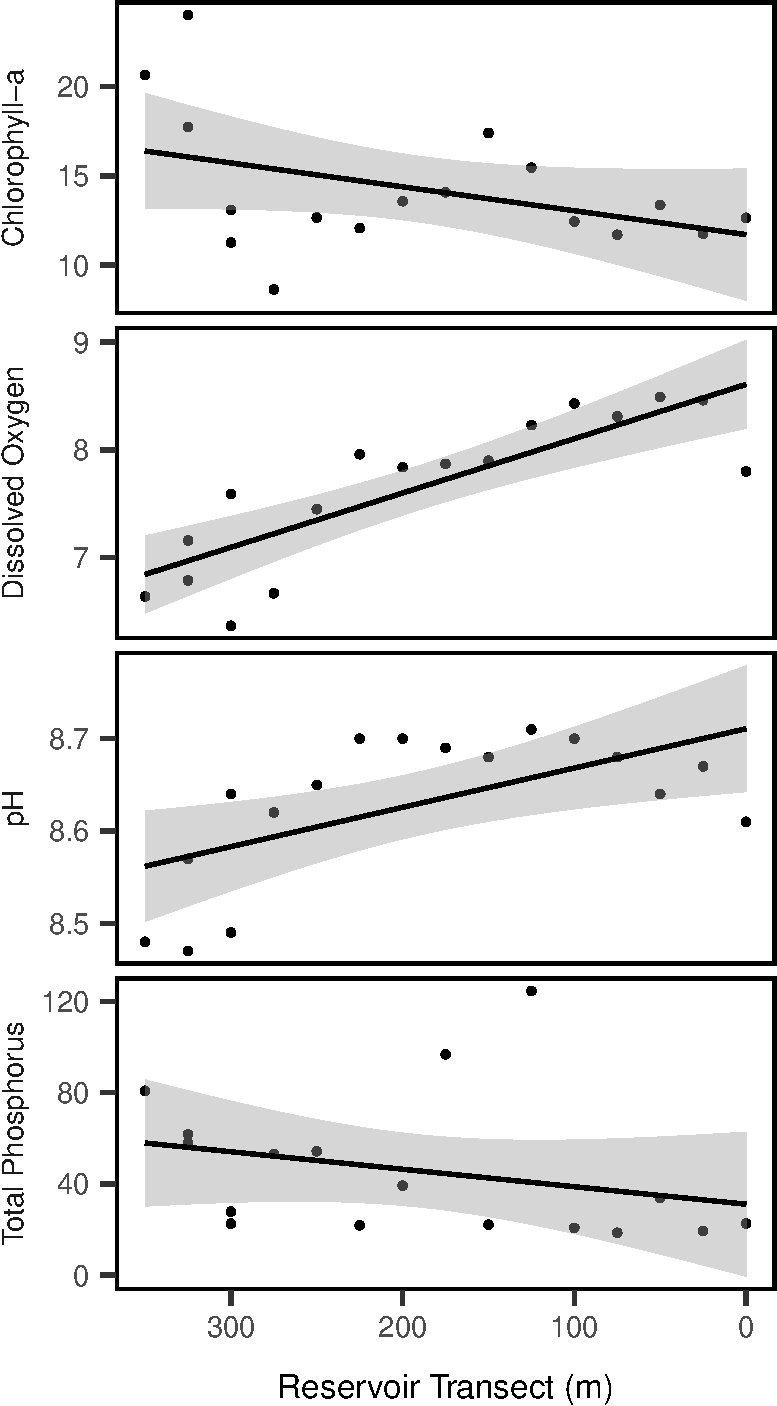
\includegraphics{ReservoirGradient_files/figure-latex/env_plot-1} \end{center}

So, there are some weak gradients, but nothing too prevailing.

\hypertarget{analyze-diversity}{%
\section{Analyze Diversity}\label{analyze-diversity}}

Now, we will analyze the bacterial diversity in the reservoir and nearby
soils to figure out how well they support different mechanisms of
community assembly.

\hypertarget{how-does-alpha-diversity-vary-along-the-reservoir}{%
\subsection{\texorpdfstring{How does \(\alpha\)-diversity vary along the
reservoir?}{How does \textbackslash{}alpha-diversity vary along the reservoir?}}\label{how-does-alpha-diversity-vary-along-the-reservoir}}

First, we use the method of rarefaction and extrapolation developed by
Chao et al.~in the iNEXT package. Note: this version of the code loads
data from the intermediate-data folder.

\begin{Shaded}
\begin{Highlighting}[]
\CommentTok{# Observed Richness}
\NormalTok{S.obs <-}\StringTok{ }\KeywordTok{rowSums}\NormalTok{((OTUs }\OperatorTok{>}\StringTok{ }\DecValTok{0}\NormalTok{) }\OperatorTok{*}\StringTok{ }\DecValTok{1}\NormalTok{)}

\CommentTok{# Simpson's Evenness}
\NormalTok{SimpE <-}\StringTok{ }\ControlFlowTok{function}\NormalTok{(}\DataTypeTok{x =} \StringTok{""}\NormalTok{)\{}
\NormalTok{  x <-}\StringTok{ }\KeywordTok{as.data.frame}\NormalTok{(x)}
\NormalTok{  D <-}\StringTok{ }\KeywordTok{diversity}\NormalTok{(x, }\StringTok{"inv"}\NormalTok{)}
\NormalTok{  S <-}\StringTok{ }\KeywordTok{sum}\NormalTok{((x }\OperatorTok{>}\StringTok{ }\DecValTok{0}\NormalTok{) }\OperatorTok{*}\StringTok{ }\DecValTok{1}\NormalTok{) }
\NormalTok{  E <-}\StringTok{ }\NormalTok{(D)}\OperatorTok{/}\NormalTok{S }
  \KeywordTok{return}\NormalTok{(E)}
\NormalTok{\}}
\NormalTok{simpsE <-}\StringTok{ }\KeywordTok{round}\NormalTok{(}\KeywordTok{apply}\NormalTok{(OTUs, }\DecValTok{1}\NormalTok{, SimpE), }\DecValTok{3}\NormalTok{)}
\NormalTok{shan <-}\StringTok{ }\KeywordTok{diversity}\NormalTok{(OTUs, }\DataTypeTok{index =} \StringTok{"shannon"}\NormalTok{)}
\NormalTok{exp.shan <-}\StringTok{ }\KeywordTok{exp}\NormalTok{(shan)}
\NormalTok{alpha.div <-}\StringTok{ }\KeywordTok{cbind}\NormalTok{(design, S.obs, simpsE, shan, exp.shan)}

\CommentTok{# define singleton estimator from Chiu and Chao 2016 PeerJ}
\KeywordTok{source}\NormalTok{(}\StringTok{"bin/Chao_functions.R"}\NormalTok{)}

\CommentTok{# # define function to extract estimated richness}
\NormalTok{singleton.apply <-}\StringTok{ }\ControlFlowTok{function}\NormalTok{(x)\{}
  \KeywordTok{singleton.Est}\NormalTok{(x, }\StringTok{"abundance"}\NormalTok{)}\OperatorTok{$}\NormalTok{corrected.data}
\NormalTok{\}}

\CommentTok{# This code is commented out, but first applies singleton correction}
\CommentTok{# then the following line runs the estimateD function }
\CommentTok{# otus.for.inext <- apply(otus.for.inext, MARGIN = 2, singleton.apply)}
\CommentTok{# divestim <- estimateD(otus.for.inext, datatype = "abundance",}
\CommentTok{#           base = "size", conf = 0.95)}
\CommentTok{# saveRDS(divestim, file = "intermediate-data/inext-output.rda")}
\NormalTok{divestim <-}\StringTok{ }\KeywordTok{readRDS}\NormalTok{(}\StringTok{"intermediate-data/inext-output.rda"}\NormalTok{)}
\NormalTok{divestim.df <-}\StringTok{ }\NormalTok{divestim }\OperatorTok\StringTok{ }
\StringTok{ }\KeywordTok{mutate}\NormalTok{(}\DataTypeTok{habitat =} \KeywordTok{str_to_title}\NormalTok{(design[}\KeywordTok{as.character}\NormalTok{(site),}\StringTok{"type"}\NormalTok{]))}
\end{Highlighting}
\end{Shaded}

Next, we'll extract the estimates for the Hill numbers at different
levels of q, which differentially weight common versus rare species.

\begin{Shaded}
\begin{Highlighting}[]
\NormalTok{hill.water <-}\StringTok{ }\NormalTok{divestim.df }\OperatorTok\StringTok{ }
\StringTok{  }\KeywordTok{filter}\NormalTok{(site }\OperatorTok\StringTok{ }\KeywordTok{rownames}\NormalTok{(OTUs)) }\OperatorTok\StringTok{ }
\StringTok{  }\KeywordTok{left_join}\NormalTok{(}\KeywordTok{rownames_to_column}\NormalTok{(alpha.div, }\DataTypeTok{var =} \StringTok{"site"}\NormalTok{)) }\OperatorTok\StringTok{ }
\StringTok{  }\KeywordTok{filter}\NormalTok{(habitat }\OperatorTok{==}\StringTok{ "Water"}\NormalTok{)}
\end{Highlighting}
\end{Shaded}

\begin{verbatim}
## Warning: Column `site` joining factor and character vector, coercing into
## character vector
\end{verbatim}

\begin{Shaded}
\begin{Highlighting}[]
\NormalTok{hill.water.rich <-}\StringTok{ }\KeywordTok{subset}\NormalTok{(hill.water, order }\OperatorTok{==}\StringTok{ }\DecValTok{0}\NormalTok{)}
\NormalTok{hill.water.shan <-}\StringTok{ }\KeywordTok{subset}\NormalTok{(hill.water, order }\OperatorTok{==}\StringTok{ }\DecValTok{1}\NormalTok{)}
\NormalTok{hill.water.simp <-}\StringTok{ }\KeywordTok{subset}\NormalTok{(hill.water, order }\OperatorTok{==}\StringTok{ }\DecValTok{2}\NormalTok{)}

\NormalTok{hill.water.mod.rich <-}\StringTok{ }\KeywordTok{lm}\NormalTok{(qD }\OperatorTok{~}\StringTok{ }\NormalTok{distance }\OperatorTok{*}\StringTok{ }\NormalTok{molecule, }\DataTypeTok{data =}\NormalTok{ hill.water.rich)}
\NormalTok{hill.water.mod.shan <-}\StringTok{ }\KeywordTok{lm}\NormalTok{(qD }\OperatorTok{~}\StringTok{ }\NormalTok{distance }\OperatorTok{*}\StringTok{ }\NormalTok{molecule, }\DataTypeTok{data =}\NormalTok{ hill.water.shan)}
\NormalTok{hill.water.mod.simp <-}\StringTok{ }\KeywordTok{lm}\NormalTok{(qD }\OperatorTok{~}\StringTok{ }\NormalTok{distance }\OperatorTok{*}\StringTok{ }\NormalTok{molecule, }\DataTypeTok{data =}\NormalTok{ hill.water.simp)}

\CommentTok{# tidy up the model output}
\NormalTok{hill.water.mods <-}\StringTok{ }\KeywordTok{as_tibble}\NormalTok{(}\KeywordTok{rbind.data.frame}\NormalTok{(}
  \KeywordTok{tidy}\NormalTok{(hill.water.mod.rich) }\OperatorTok\StringTok{ }\KeywordTok{add_column}\NormalTok{(}\DataTypeTok{Diversity =} \StringTok{"Richness"}\NormalTok{),}
  \KeywordTok{tidy}\NormalTok{(hill.water.mod.shan) }\OperatorTok\StringTok{ }\KeywordTok{add_column}\NormalTok{(}\DataTypeTok{Diversity =} \StringTok{"Shannon"}\NormalTok{),}
  \KeywordTok{tidy}\NormalTok{(hill.water.mod.simp) }\OperatorTok\StringTok{ }\KeywordTok{add_column}\NormalTok{(}\DataTypeTok{Diversity =} \StringTok{"Simpson"}\NormalTok{)}
\NormalTok{))}
\end{Highlighting}
\end{Shaded}

\begin{Shaded}
\begin{Highlighting}[]
\CommentTok{# Summary table of the model results. }
\NormalTok{hill.water.mods }\OperatorTok\StringTok{ }
\StringTok{  }\KeywordTok{group_by}\NormalTok{(Diversity) }\OperatorTok\StringTok{ }
\StringTok{  }\KeywordTok{rename}\NormalTok{(}\StringTok{"Term"}\NormalTok{ =}\StringTok{ }\NormalTok{term, }
         \StringTok{"Estimate"}\NormalTok{ =}\StringTok{ }\NormalTok{estimate, }
         \StringTok{"Std. Error"}\NormalTok{ =}\StringTok{ }\NormalTok{std.error, }
         \StringTok{"Statistic"}\NormalTok{ =}\StringTok{ }\NormalTok{statistic, }
         \StringTok{"p-value"}\NormalTok{ =}\StringTok{ }\NormalTok{p.value) }\OperatorTok\StringTok{ }
\StringTok{  }\KeywordTok{select}\NormalTok{(Diversity, }\KeywordTok{everything}\NormalTok{()) }\OperatorTok\StringTok{ }
\StringTok{  }\KeywordTok{pander}\NormalTok{(}\DataTypeTok{round =} \DecValTok{4}\NormalTok{)}
\end{Highlighting}
\end{Shaded}

\begin{longtable}[]{@{}cccccc@{}}
\toprule
\begin{minipage}[b]{0.12\columnwidth}\centering
Diversity\strut
\end{minipage} & \begin{minipage}[b]{0.23\columnwidth}\centering
Term\strut
\end{minipage} & \begin{minipage}[b]{0.11\columnwidth}\centering
Estimate\strut
\end{minipage} & \begin{minipage}[b]{0.13\columnwidth}\centering
Std. Error\strut
\end{minipage} & \begin{minipage}[b]{0.12\columnwidth}\centering
Statistic\strut
\end{minipage} & \begin{minipage}[b]{0.12\columnwidth}\centering
p-value\strut
\end{minipage}\tabularnewline
\midrule
\endhead
\begin{minipage}[t]{0.12\columnwidth}\centering
Richness\strut
\end{minipage} & \begin{minipage}[t]{0.23\columnwidth}\centering
(Intercept)\strut
\end{minipage} & \begin{minipage}[t]{0.11\columnwidth}\centering
1497\strut
\end{minipage} & \begin{minipage}[t]{0.13\columnwidth}\centering
100.6\strut
\end{minipage} & \begin{minipage}[t]{0.12\columnwidth}\centering
14.88\strut
\end{minipage} & \begin{minipage}[t]{0.12\columnwidth}\centering
0\strut
\end{minipage}\tabularnewline
\begin{minipage}[t]{0.12\columnwidth}\centering
Richness\strut
\end{minipage} & \begin{minipage}[t]{0.23\columnwidth}\centering
distance\strut
\end{minipage} & \begin{minipage}[t]{0.11\columnwidth}\centering
-3.176\strut
\end{minipage} & \begin{minipage}[t]{0.13\columnwidth}\centering
0.4976\strut
\end{minipage} & \begin{minipage}[t]{0.12\columnwidth}\centering
-6.381\strut
\end{minipage} & \begin{minipage}[t]{0.12\columnwidth}\centering
0\strut
\end{minipage}\tabularnewline
\begin{minipage}[t]{0.12\columnwidth}\centering
Richness\strut
\end{minipage} & \begin{minipage}[t]{0.23\columnwidth}\centering
moleculeRNA\strut
\end{minipage} & \begin{minipage}[t]{0.11\columnwidth}\centering
-1170\strut
\end{minipage} & \begin{minipage}[t]{0.13\columnwidth}\centering
142.3\strut
\end{minipage} & \begin{minipage}[t]{0.12\columnwidth}\centering
-8.222\strut
\end{minipage} & \begin{minipage}[t]{0.12\columnwidth}\centering
0\strut
\end{minipage}\tabularnewline
\begin{minipage}[t]{0.12\columnwidth}\centering
Richness\strut
\end{minipage} & \begin{minipage}[t]{0.23\columnwidth}\centering
distance:moleculeRNA\strut
\end{minipage} & \begin{minipage}[t]{0.11\columnwidth}\centering
2.985\strut
\end{minipage} & \begin{minipage}[t]{0.13\columnwidth}\centering
0.7003\strut
\end{minipage} & \begin{minipage}[t]{0.12\columnwidth}\centering
4.263\strut
\end{minipage} & \begin{minipage}[t]{0.12\columnwidth}\centering
3e-04\strut
\end{minipage}\tabularnewline
\begin{minipage}[t]{0.12\columnwidth}\centering
Shannon\strut
\end{minipage} & \begin{minipage}[t]{0.23\columnwidth}\centering
(Intercept)\strut
\end{minipage} & \begin{minipage}[t]{0.11\columnwidth}\centering
153.7\strut
\end{minipage} & \begin{minipage}[t]{0.13\columnwidth}\centering
19.41\strut
\end{minipage} & \begin{minipage}[t]{0.12\columnwidth}\centering
7.921\strut
\end{minipage} & \begin{minipage}[t]{0.12\columnwidth}\centering
0\strut
\end{minipage}\tabularnewline
\begin{minipage}[t]{0.12\columnwidth}\centering
Shannon\strut
\end{minipage} & \begin{minipage}[t]{0.23\columnwidth}\centering
distance\strut
\end{minipage} & \begin{minipage}[t]{0.11\columnwidth}\centering
-0.2941\strut
\end{minipage} & \begin{minipage}[t]{0.13\columnwidth}\centering
0.096\strut
\end{minipage} & \begin{minipage}[t]{0.12\columnwidth}\centering
-3.062\strut
\end{minipage} & \begin{minipage}[t]{0.12\columnwidth}\centering
0.0053\strut
\end{minipage}\tabularnewline
\begin{minipage}[t]{0.12\columnwidth}\centering
Shannon\strut
\end{minipage} & \begin{minipage}[t]{0.23\columnwidth}\centering
moleculeRNA\strut
\end{minipage} & \begin{minipage}[t]{0.11\columnwidth}\centering
-123.9\strut
\end{minipage} & \begin{minipage}[t]{0.13\columnwidth}\centering
27.46\strut
\end{minipage} & \begin{minipage}[t]{0.12\columnwidth}\centering
-4.513\strut
\end{minipage} & \begin{minipage}[t]{0.12\columnwidth}\centering
1e-04\strut
\end{minipage}\tabularnewline
\begin{minipage}[t]{0.12\columnwidth}\centering
Shannon\strut
\end{minipage} & \begin{minipage}[t]{0.23\columnwidth}\centering
distance:moleculeRNA\strut
\end{minipage} & \begin{minipage}[t]{0.11\columnwidth}\centering
0.2457\strut
\end{minipage} & \begin{minipage}[t]{0.13\columnwidth}\centering
0.1352\strut
\end{minipage} & \begin{minipage}[t]{0.12\columnwidth}\centering
1.818\strut
\end{minipage} & \begin{minipage}[t]{0.12\columnwidth}\centering
0.0815\strut
\end{minipage}\tabularnewline
\begin{minipage}[t]{0.12\columnwidth}\centering
Simpson\strut
\end{minipage} & \begin{minipage}[t]{0.23\columnwidth}\centering
(Intercept)\strut
\end{minipage} & \begin{minipage}[t]{0.11\columnwidth}\centering
55.44\strut
\end{minipage} & \begin{minipage}[t]{0.13\columnwidth}\centering
6.47\strut
\end{minipage} & \begin{minipage}[t]{0.12\columnwidth}\centering
8.57\strut
\end{minipage} & \begin{minipage}[t]{0.12\columnwidth}\centering
0\strut
\end{minipage}\tabularnewline
\begin{minipage}[t]{0.12\columnwidth}\centering
Simpson\strut
\end{minipage} & \begin{minipage}[t]{0.23\columnwidth}\centering
distance\strut
\end{minipage} & \begin{minipage}[t]{0.11\columnwidth}\centering
-0.0783\strut
\end{minipage} & \begin{minipage}[t]{0.13\columnwidth}\centering
0.032\strut
\end{minipage} & \begin{minipage}[t]{0.12\columnwidth}\centering
-2.446\strut
\end{minipage} & \begin{minipage}[t]{0.12\columnwidth}\centering
0.0221\strut
\end{minipage}\tabularnewline
\begin{minipage}[t]{0.12\columnwidth}\centering
Simpson\strut
\end{minipage} & \begin{minipage}[t]{0.23\columnwidth}\centering
moleculeRNA\strut
\end{minipage} & \begin{minipage}[t]{0.11\columnwidth}\centering
-36.78\strut
\end{minipage} & \begin{minipage}[t]{0.13\columnwidth}\centering
9.151\strut
\end{minipage} & \begin{minipage}[t]{0.12\columnwidth}\centering
-4.019\strut
\end{minipage} & \begin{minipage}[t]{0.12\columnwidth}\centering
5e-04\strut
\end{minipage}\tabularnewline
\begin{minipage}[t]{0.12\columnwidth}\centering
Simpson\strut
\end{minipage} & \begin{minipage}[t]{0.23\columnwidth}\centering
distance:moleculeRNA\strut
\end{minipage} & \begin{minipage}[t]{0.11\columnwidth}\centering
0.0402\strut
\end{minipage} & \begin{minipage}[t]{0.13\columnwidth}\centering
0.045\strut
\end{minipage} & \begin{minipage}[t]{0.12\columnwidth}\centering
0.8918\strut
\end{minipage} & \begin{minipage}[t]{0.12\columnwidth}\centering
0.3813\strut
\end{minipage}\tabularnewline
\bottomrule
\end{longtable}

\hypertarget{figure-2-diversity-patterns-along-the-gradient}{%
\section{Figure 2: diversity patterns along the
gradient}\label{figure-2-diversity-patterns-along-the-gradient}}

\hypertarget{panel-a-alpha-diversity}{%
\subsection{Panel a: alpha diversity}\label{panel-a-alpha-diversity}}

First, generate panel a for Figure 2.

\begin{Shaded}
\begin{Highlighting}[]
\CommentTok{# postitions for labels}
\NormalTok{xpos =}\StringTok{ }\KeywordTok{max}\NormalTok{((}\KeywordTok{na.omit}\NormalTok{(hill.water}\OperatorTok{$}\NormalTok{distance)))}
\NormalTok{yposDNA =}\StringTok{ }\KeywordTok{predict}\NormalTok{(hill.water.mod.rich, }\DataTypeTok{newdata =} \KeywordTok{data.frame}\NormalTok{(}\DataTypeTok{distance =} \DecValTok{0}\NormalTok{, }\DataTypeTok{molecule =} \StringTok{"DNA"}\NormalTok{))}
\NormalTok{yposRNA =}\StringTok{ }\KeywordTok{predict}\NormalTok{(hill.water.mod.rich, }\DataTypeTok{newdata =} \KeywordTok{data.frame}\NormalTok{(}\DataTypeTok{distance =} \DecValTok{0}\NormalTok{, }\DataTypeTok{molecule =} \StringTok{"RNA"}\NormalTok{))}

\CommentTok{# Here we generate panel a for Figure 2}
\NormalTok{alpha.fig <-}\StringTok{ }\NormalTok{hill.water }\OperatorTok\StringTok{ }\KeywordTok{filter}\NormalTok{(type }\OperatorTok{==}\StringTok{ "water"}\NormalTok{, order }\OperatorTok{==}\StringTok{ }\DecValTok{0}\NormalTok{) }\OperatorTok\StringTok{ }
\StringTok{  }\KeywordTok{mutate}\NormalTok{(}\DataTypeTok{molecule =} \KeywordTok{ifelse}\NormalTok{(molecule }\OperatorTok{==}\StringTok{ "DNA"}\NormalTok{, }\StringTok{"Total"}\NormalTok{, }\StringTok{"Active"}\NormalTok{)) }\OperatorTok\StringTok{ }
\StringTok{  }\KeywordTok{ggplot}\NormalTok{(}\KeywordTok{aes}\NormalTok{(}\DataTypeTok{x =}\NormalTok{ distance, }\DataTypeTok{y =}\NormalTok{ qD, }
             \DataTypeTok{ymin =}\NormalTok{ qD.LCL, }\DataTypeTok{ymax =}\NormalTok{ qD.UCL,}
             \DataTypeTok{shape =}\NormalTok{ molecule)) }\OperatorTok{+}\StringTok{ }
\StringTok{  }\CommentTok{# geom_errorbar(size = .5, width = 10, alpha = 0.5) +}
\StringTok{  }\KeywordTok{geom_smooth}\NormalTok{(}\DataTypeTok{method =} \StringTok{"lm"}\NormalTok{, }\KeywordTok{aes}\NormalTok{(}\DataTypeTok{linetype =}\NormalTok{ molecule), }\DataTypeTok{color =} \StringTok{"black"}\NormalTok{) }\OperatorTok{+}
\StringTok{  }\KeywordTok{geom_point}\NormalTok{(}\DataTypeTok{size =}\DecValTok{3}\NormalTok{, }\DataTypeTok{alpha =} \FloatTok{0.8}\NormalTok{) }\OperatorTok{+}\StringTok{ }
\StringTok{  }\KeywordTok{labs}\NormalTok{(}\DataTypeTok{x =} \StringTok{"Reservoir distance (m)"}\NormalTok{,}
       \DataTypeTok{y =} \StringTok{"Estimated richness"}\NormalTok{) }\OperatorTok{+}
\StringTok{  }\KeywordTok{scale_y_continuous}\NormalTok{(}\DataTypeTok{breaks =} \KeywordTok{seq}\NormalTok{(}\DecValTok{0}\NormalTok{, }\DecValTok{2000}\NormalTok{, }\DataTypeTok{by =} \DecValTok{500}\NormalTok{)) }\OperatorTok{+}
\StringTok{  }\KeywordTok{scale_x_continuous}\NormalTok{(}\DataTypeTok{limits =} \KeywordTok{c}\NormalTok{(}\OperatorTok{-}\DecValTok{49}\NormalTok{, }\DecValTok{350}\NormalTok{)) }\OperatorTok{+}
\StringTok{  }\KeywordTok{theme}\NormalTok{(}\DataTypeTok{legend.position =} \StringTok{"none"}\NormalTok{) }\OperatorTok{+}
\StringTok{  }\KeywordTok{guides}\NormalTok{(}\DataTypeTok{fill =} \KeywordTok{guide_legend}\NormalTok{(}\DataTypeTok{override.aes=}\KeywordTok{list}\NormalTok{(}\DataTypeTok{fill=}\OtherTok{NA}\NormalTok{))) }\OperatorTok{+}
\StringTok{  }\KeywordTok{annotate}\NormalTok{(}\StringTok{"text"}\NormalTok{, }\DataTypeTok{x =} \DecValTok{-33}\NormalTok{, }\DataTypeTok{y =}\NormalTok{ yposRNA , }
           \DataTypeTok{label =} \StringTok{"Active"}\NormalTok{, }\DataTypeTok{size =} \DecValTok{5}\NormalTok{) }\OperatorTok{+}
\StringTok{  }\KeywordTok{annotate}\NormalTok{(}\StringTok{"text"}\NormalTok{, }\DataTypeTok{x =} \DecValTok{-33}\NormalTok{, }\DataTypeTok{y =}\NormalTok{ yposDNA , }
           \DataTypeTok{label =} \StringTok{"Total"}\NormalTok{, }\DataTypeTok{size =} \DecValTok{5}\NormalTok{) }\OperatorTok{+}
\StringTok{  }\KeywordTok{annotate}\NormalTok{(}\DataTypeTok{geom =} \StringTok{"text"}\NormalTok{, }\DataTypeTok{x =}\NormalTok{ xpos, }\DataTypeTok{y =} \DecValTok{2000}\NormalTok{, }\DataTypeTok{hjust =} \DecValTok{1}\NormalTok{, }\DataTypeTok{vjust =} \DecValTok{1}\NormalTok{, }\DataTypeTok{size =} \DecValTok{5}\NormalTok{,}
           \DataTypeTok{label =} \KeywordTok{paste0}\NormalTok{(}\StringTok{"r^2== "}\NormalTok{,}\KeywordTok{round}\NormalTok{(}\KeywordTok{summary}\NormalTok{(hill.water.mod.rich)}\OperatorTok{$}\NormalTok{r.squared, }\DecValTok{2}\NormalTok{)), }\DataTypeTok{parse =}\NormalTok{ T)}
\end{Highlighting}
\end{Shaded}

\hypertarget{similarity-to-terrestrial-habitat-across-gradient-terrestrial-influence}{%
\subsection{Similarity To Terrestrial Habitat Across Gradient
(Terrestrial
Influence)}\label{similarity-to-terrestrial-habitat-across-gradient-terrestrial-influence}}

Here, we fit a linear model to the similarity of the aquatic community
to the soil community.

\begin{Shaded}
\begin{Highlighting}[]
\CommentTok{# Similarity to Soil Sample}
\NormalTok{UL.bray      <-}\StringTok{ }\DecValTok{1}\OperatorTok{-}\KeywordTok{as.matrix}\NormalTok{(}\KeywordTok{vegdist}\NormalTok{(OTUsREL.log, }\DataTypeTok{method=}\StringTok{"bray"}\NormalTok{))}
\NormalTok{UL.bray.lake <-}\StringTok{ }\NormalTok{UL.bray[}\OperatorTok{-}\KeywordTok{c}\NormalTok{(}\DecValTok{1}\OperatorTok{:}\DecValTok{3}\NormalTok{), }\DecValTok{1}\OperatorTok{:}\DecValTok{3}\NormalTok{] }
\NormalTok{bray.mean    <-}\StringTok{ }\KeywordTok{round}\NormalTok{(}\KeywordTok{apply}\NormalTok{(UL.bray.lake, }\DecValTok{1}\NormalTok{, mean), }\DecValTok{3}\NormalTok{)}
\NormalTok{bray.se      <-}\StringTok{ }\KeywordTok{round}\NormalTok{(}\KeywordTok{apply}\NormalTok{(UL.bray.lake, }\DecValTok{1}\NormalTok{, se), }\DecValTok{3}\NormalTok{)}
\NormalTok{UL.sim       <-}\StringTok{ }\KeywordTok{cbind}\NormalTok{(design[}\OperatorTok{-}\KeywordTok{c}\NormalTok{(}\DecValTok{1}\OperatorTok{:}\DecValTok{3}\NormalTok{), ], bray.mean, bray.se)}

\CommentTok{# Calculate Linear Model}
\NormalTok{model.terr <-}\StringTok{ }\KeywordTok{lm}\NormalTok{(bray.mean }\OperatorTok{~}\StringTok{ }\NormalTok{distance }\OperatorTok{*}\StringTok{ }\NormalTok{molecule, }\DataTypeTok{data =}\NormalTok{ UL.sim)}
\KeywordTok{predict}\NormalTok{(model.terr, }\DataTypeTok{newdata =} \KeywordTok{data.frame}\NormalTok{(}\DataTypeTok{distance =} \DecValTok{0}\NormalTok{, }\DataTypeTok{molecule =} \KeywordTok{c}\NormalTok{(}\StringTok{"RNA"}\NormalTok{, }\StringTok{"DNA"}\NormalTok{)))}
\end{Highlighting}
\end{Shaded}

\begin{verbatim}
##          1          2 
## 0.03090104 0.17193131
\end{verbatim}

\begin{Shaded}
\begin{Highlighting}[]
\KeywordTok{pander}\NormalTok{(model.terr)}
\end{Highlighting}
\end{Shaded}

\begin{longtable}[]{@{}ccccc@{}}
\caption{Fitting linear model: bray.mean \textasciitilde{} distance *
molecule}\tabularnewline
\toprule
\begin{minipage}[b]{0.31\columnwidth}\centering
~\strut
\end{minipage} & \begin{minipage}[b]{0.15\columnwidth}\centering
Estimate\strut
\end{minipage} & \begin{minipage}[b]{0.15\columnwidth}\centering
Std. Error\strut
\end{minipage} & \begin{minipage}[b]{0.11\columnwidth}\centering
t value\strut
\end{minipage} & \begin{minipage}[b]{0.14\columnwidth}\centering
Pr(\textgreater{}\textbar{}t\textbar{})\strut
\end{minipage}\tabularnewline
\midrule
\endfirsthead
\toprule
\begin{minipage}[b]{0.31\columnwidth}\centering
~\strut
\end{minipage} & \begin{minipage}[b]{0.15\columnwidth}\centering
Estimate\strut
\end{minipage} & \begin{minipage}[b]{0.15\columnwidth}\centering
Std. Error\strut
\end{minipage} & \begin{minipage}[b]{0.11\columnwidth}\centering
t value\strut
\end{minipage} & \begin{minipage}[b]{0.14\columnwidth}\centering
Pr(\textgreater{}\textbar{}t\textbar{})\strut
\end{minipage}\tabularnewline
\midrule
\endhead
\begin{minipage}[t]{0.31\columnwidth}\centering
\textbf{(Intercept)}\strut
\end{minipage} & \begin{minipage}[t]{0.15\columnwidth}\centering
0.1719\strut
\end{minipage} & \begin{minipage}[t]{0.15\columnwidth}\centering
0.0138\strut
\end{minipage} & \begin{minipage}[t]{0.11\columnwidth}\centering
12.46\strut
\end{minipage} & \begin{minipage}[t]{0.14\columnwidth}\centering
5.707e-12\strut
\end{minipage}\tabularnewline
\begin{minipage}[t]{0.31\columnwidth}\centering
\textbf{distance}\strut
\end{minipage} & \begin{minipage}[t]{0.15\columnwidth}\centering
-0.0003988\strut
\end{minipage} & \begin{minipage}[t]{0.15\columnwidth}\centering
6.827e-05\strut
\end{minipage} & \begin{minipage}[t]{0.11\columnwidth}\centering
-5.841\strut
\end{minipage} & \begin{minipage}[t]{0.14\columnwidth}\centering
5.045e-06\strut
\end{minipage}\tabularnewline
\begin{minipage}[t]{0.31\columnwidth}\centering
\textbf{moleculeRNA}\strut
\end{minipage} & \begin{minipage}[t]{0.15\columnwidth}\centering
-0.141\strut
\end{minipage} & \begin{minipage}[t]{0.15\columnwidth}\centering
0.01952\strut
\end{minipage} & \begin{minipage}[t]{0.11\columnwidth}\centering
-7.226\strut
\end{minipage} & \begin{minipage}[t]{0.14\columnwidth}\centering
1.821e-07\strut
\end{minipage}\tabularnewline
\begin{minipage}[t]{0.31\columnwidth}\centering
\textbf{distance:moleculeRNA}\strut
\end{minipage} & \begin{minipage}[t]{0.15\columnwidth}\centering
0.0003839\strut
\end{minipage} & \begin{minipage}[t]{0.15\columnwidth}\centering
9.608e-05\strut
\end{minipage} & \begin{minipage}[t]{0.11\columnwidth}\centering
3.996\strut
\end{minipage} & \begin{minipage}[t]{0.14\columnwidth}\centering
0.0005324\strut
\end{minipage}\tabularnewline
\bottomrule
\end{longtable}

\hypertarget{panel-b-beta-diversity}{%
\subsection{Panel b: beta-diversity}\label{panel-b-beta-diversity}}

\begin{Shaded}
\begin{Highlighting}[]
\NormalTok{ypred.act <-}\StringTok{ }\KeywordTok{predict}\NormalTok{(model.terr, }\DataTypeTok{newdata =} \KeywordTok{data.frame}\NormalTok{(}\DataTypeTok{distance =} \DecValTok{0}\NormalTok{, }\DataTypeTok{molecule =} \StringTok{"RNA"}\NormalTok{))}
\NormalTok{ypred.tot <-}\StringTok{ }\KeywordTok{predict}\NormalTok{(model.terr, }\DataTypeTok{newdata =} \KeywordTok{data.frame}\NormalTok{(}\DataTypeTok{distance =} \DecValTok{0}\NormalTok{, }\DataTypeTok{molecule =} \StringTok{"DNA"}\NormalTok{))}

\CommentTok{# make plot}
\NormalTok{similarity.plot <-}\StringTok{ }\NormalTok{UL.sim }\OperatorTok\StringTok{ }
\StringTok{  }\KeywordTok{mutate}\NormalTok{(}\DataTypeTok{molecule =} \KeywordTok{ifelse}\NormalTok{(UL.sim}\OperatorTok{$}\NormalTok{molecule }\OperatorTok{==}\StringTok{ "DNA"}\NormalTok{, }\StringTok{"Total"}\NormalTok{, }\StringTok{"Active"}\NormalTok{)) }\OperatorTok\StringTok{ }
\StringTok{  }\KeywordTok{ggplot}\NormalTok{(}\KeywordTok{aes}\NormalTok{(}\DataTypeTok{x =}\NormalTok{ distance, }\DataTypeTok{y =}\NormalTok{ bray.mean, }\DataTypeTok{shape =}\NormalTok{ molecule)) }\OperatorTok{+}
\StringTok{  }\KeywordTok{geom_smooth}\NormalTok{(}\DataTypeTok{method =} \StringTok{"lm"}\NormalTok{, }\KeywordTok{aes}\NormalTok{(}\DataTypeTok{linetype =}\NormalTok{ molecule), }\DataTypeTok{color =} \StringTok{"black"}\NormalTok{, }\DataTypeTok{show.legend =}\NormalTok{ T) }\OperatorTok{+}\StringTok{ }
\StringTok{  }\KeywordTok{geom_point}\NormalTok{(}\DataTypeTok{alpha =} \FloatTok{0.8}\NormalTok{, }\DataTypeTok{size =} \DecValTok{3}\NormalTok{, }\DataTypeTok{show.legend =}\NormalTok{ T) }\OperatorTok{+}\StringTok{ }
\StringTok{  }\KeywordTok{labs}\NormalTok{(}\DataTypeTok{y =} \KeywordTok{str_wrap}\NormalTok{(}\StringTok{"Percent similarity to soil community"}\NormalTok{, }\DataTypeTok{width =} \DecValTok{20}\NormalTok{), }
       \DataTypeTok{x =} \StringTok{"Reservoir distance (m)"}\NormalTok{) }\OperatorTok{+}\StringTok{ }
\StringTok{  }\KeywordTok{theme}\NormalTok{(}\DataTypeTok{legend.position =} \StringTok{"none"}\NormalTok{) }\OperatorTok{+}
\StringTok{  }\KeywordTok{scale_x_continuous}\NormalTok{(}\DataTypeTok{limits =} \KeywordTok{c}\NormalTok{(}\OperatorTok{-}\DecValTok{49}\NormalTok{,}\DecValTok{350}\NormalTok{)) }\OperatorTok{+}\StringTok{ }
\StringTok{  }\KeywordTok{annotate}\NormalTok{(}\DataTypeTok{geom =} \StringTok{"text"}\NormalTok{, }\DataTypeTok{x =} \DecValTok{350}\NormalTok{, }\DataTypeTok{y =} \KeywordTok{max}\NormalTok{(UL.sim}\OperatorTok{$}\NormalTok{bray.mean), }\DataTypeTok{hjust =} \DecValTok{1}\NormalTok{, }\DataTypeTok{vjust =} \DecValTok{1}\NormalTok{, }\DataTypeTok{size =} \DecValTok{5}\NormalTok{,}
           \DataTypeTok{label =} \KeywordTok{paste0}\NormalTok{(}\StringTok{"r^2== "}\NormalTok{,}\KeywordTok{round}\NormalTok{(}\KeywordTok{summary}\NormalTok{(model.terr)}\OperatorTok{$}\NormalTok{r.squared, }\DecValTok{2}\NormalTok{)), }\DataTypeTok{parse =}\NormalTok{ T) }\OperatorTok{+}
\StringTok{  }\KeywordTok{annotate}\NormalTok{(}\StringTok{"text"}\NormalTok{, }\DataTypeTok{x =} \DecValTok{-33}\NormalTok{, }\DataTypeTok{y =}\NormalTok{ ypred.act, }\DataTypeTok{label =} \StringTok{"Active"}\NormalTok{, }\DataTypeTok{size =} \DecValTok{5}\NormalTok{) }\OperatorTok{+}
\StringTok{  }\KeywordTok{annotate}\NormalTok{(}\StringTok{"text"}\NormalTok{, }\DataTypeTok{x =} \DecValTok{-33}\NormalTok{, }\DataTypeTok{y =}\NormalTok{ ypred.tot, }\DataTypeTok{label =} \StringTok{"Total"}\NormalTok{, }\DataTypeTok{size =} \DecValTok{5}\NormalTok{)}
\end{Highlighting}
\end{Shaded}

\hypertarget{create-combined-figure}{%
\subsection{Create combined figure}\label{create-combined-figure}}

\begin{Shaded}
\begin{Highlighting}[]
\KeywordTok{plot_grid}\NormalTok{(alpha.fig }\OperatorTok{+}\StringTok{ }\KeywordTok{labs}\NormalTok{(}\DataTypeTok{x =} \StringTok{""}\NormalTok{), similarity.plot, }
          \DataTypeTok{align =} \StringTok{"hv"}\NormalTok{,}
          \DataTypeTok{labels =} \StringTok{"auto"}\NormalTok{, }\DataTypeTok{ncol =} \DecValTok{1}\NormalTok{) }\OperatorTok{+}
\StringTok{  }\KeywordTok{ggsave}\NormalTok{(}\StringTok{"figures/Figure2.pdf"}\NormalTok{)}
\end{Highlighting}
\end{Shaded}

\begin{center}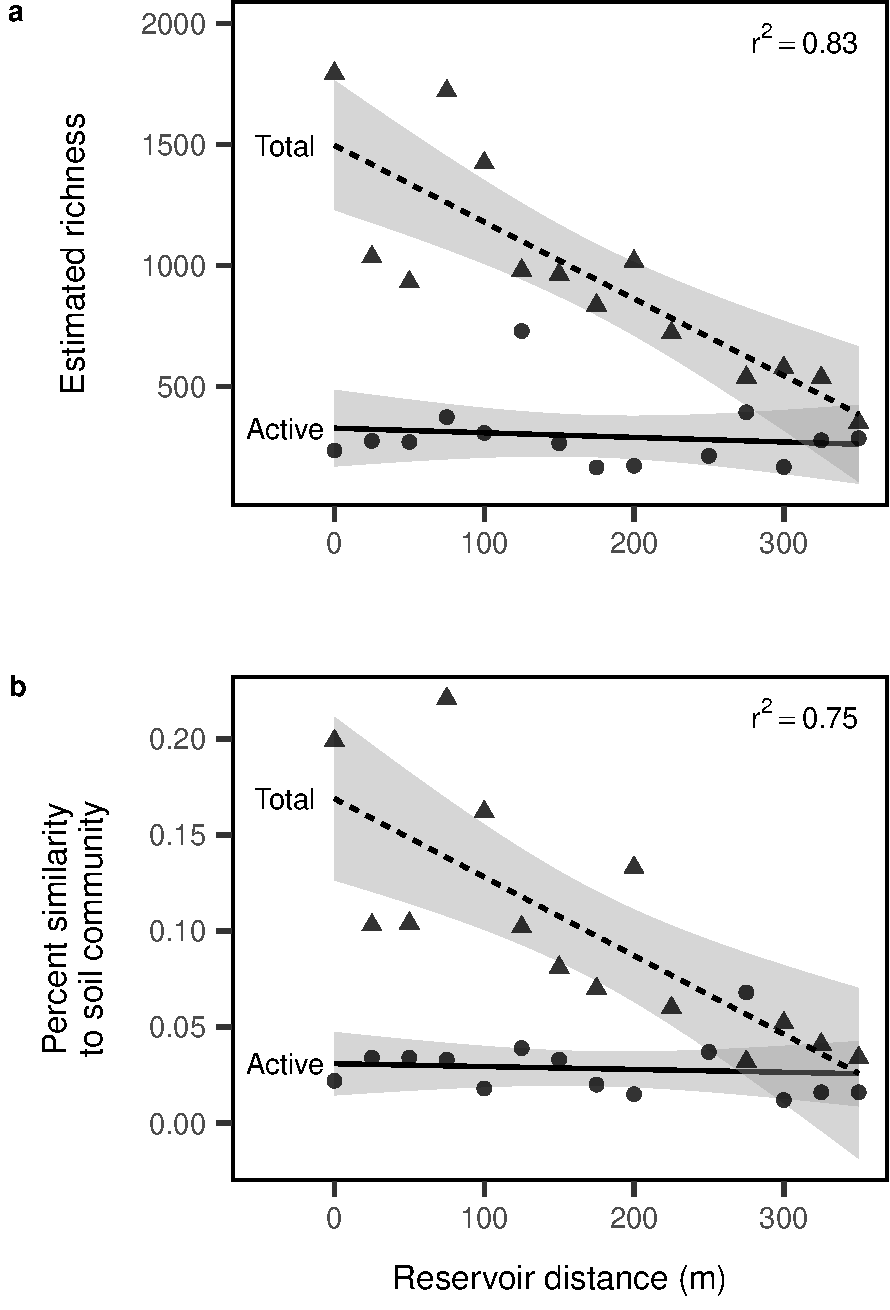
\includegraphics{ReservoirGradient_files/figure-latex/combined-plots-1} \end{center}

\hypertarget{figure-s3-are-the-aquatic-samples-nested-subsets-of-the-soil}{%
\section{Figure S3: Are the aquatic samples nested subsets of the
soil?}\label{figure-s3-are-the-aquatic-samples-nested-subsets-of-the-soil}}

\begin{Shaded}
\begin{Highlighting}[]
\NormalTok{betapart.sor <-}\StringTok{ }\KeywordTok{beta.pair}\NormalTok{(}\KeywordTok{decostand}\NormalTok{(OTUs, }\DataTypeTok{method =} \StringTok{"pa"}\NormalTok{), }\StringTok{"sorensen"}\NormalTok{)}

\NormalTok{nest.lake <-}\StringTok{ }\KeywordTok{as.matrix}\NormalTok{(betapart.sor}\OperatorTok{$}\NormalTok{beta.sne)[}\OperatorTok{-}\KeywordTok{c}\NormalTok{(}\DecValTok{1}\OperatorTok{:}\DecValTok{3}\NormalTok{), }\DecValTok{1}\OperatorTok{:}\DecValTok{3}\NormalTok{] }
\NormalTok{nest.mean    <-}\StringTok{ }\KeywordTok{round}\NormalTok{(}\KeywordTok{apply}\NormalTok{(nest.lake, }\DecValTok{1}\NormalTok{, mean), }\DecValTok{3}\NormalTok{)}
\NormalTok{nest.se      <-}\StringTok{ }\KeywordTok{round}\NormalTok{(}\KeywordTok{apply}\NormalTok{(nest.lake, }\DecValTok{1}\NormalTok{, se), }\DecValTok{3}\NormalTok{)}
\NormalTok{UL.nest       <-}\StringTok{ }\KeywordTok{cbind}\NormalTok{(design[}\OperatorTok{-}\KeywordTok{c}\NormalTok{(}\DecValTok{1}\OperatorTok{:}\DecValTok{3}\NormalTok{), ], nest.mean, nest.se)}

\NormalTok{turn.lake <-}\StringTok{ }\KeywordTok{as.matrix}\NormalTok{(betapart.sor}\OperatorTok{$}\NormalTok{beta.sim)[}\OperatorTok{-}\KeywordTok{c}\NormalTok{(}\DecValTok{1}\OperatorTok{:}\DecValTok{3}\NormalTok{), }\DecValTok{1}\OperatorTok{:}\DecValTok{3}\NormalTok{] }
\NormalTok{turn.mean    <-}\StringTok{ }\KeywordTok{round}\NormalTok{(}\KeywordTok{apply}\NormalTok{(turn.lake, }\DecValTok{1}\NormalTok{, mean), }\DecValTok{3}\NormalTok{)}
\NormalTok{turn.se      <-}\StringTok{ }\KeywordTok{round}\NormalTok{(}\KeywordTok{apply}\NormalTok{(turn.lake, }\DecValTok{1}\NormalTok{, se), }\DecValTok{3}\NormalTok{)}
\NormalTok{UL.turn       <-}\StringTok{ }\KeywordTok{cbind}\NormalTok{(design[}\OperatorTok{-}\KeywordTok{c}\NormalTok{(}\DecValTok{1}\OperatorTok{:}\DecValTok{3}\NormalTok{), ], turn.mean, turn.se)}

\NormalTok{sor.lake <-}\StringTok{ }\KeywordTok{as.matrix}\NormalTok{(betapart.sor}\OperatorTok{$}\NormalTok{beta.sor)[}\OperatorTok{-}\KeywordTok{c}\NormalTok{(}\DecValTok{1}\OperatorTok{:}\DecValTok{3}\NormalTok{), }\DecValTok{1}\OperatorTok{:}\DecValTok{3}\NormalTok{] }
\NormalTok{sor.mean    <-}\StringTok{ }\KeywordTok{round}\NormalTok{(}\KeywordTok{apply}\NormalTok{(sor.lake, }\DecValTok{1}\NormalTok{, mean), }\DecValTok{3}\NormalTok{)}
\NormalTok{sor.se      <-}\StringTok{ }\KeywordTok{round}\NormalTok{(}\KeywordTok{apply}\NormalTok{(sor.lake, }\DecValTok{1}\NormalTok{, se), }\DecValTok{3}\NormalTok{)}
\NormalTok{UL.sor       <-}\StringTok{ }\KeywordTok{cbind}\NormalTok{(design[}\OperatorTok{-}\KeywordTok{c}\NormalTok{(}\DecValTok{1}\OperatorTok{:}\DecValTok{3}\NormalTok{), ], sor.mean, sor.se)}

\KeywordTok{left_join}\NormalTok{(UL.nest, UL.turn) }\OperatorTok\StringTok{ }\KeywordTok{left_join}\NormalTok{(UL.sor) }\OperatorTok\StringTok{ }
\StringTok{  }\KeywordTok{mutate}\NormalTok{(}\DataTypeTok{molecule =} \KeywordTok{ifelse}\NormalTok{(molecule }\OperatorTok{==}\StringTok{ "DNA"}\NormalTok{, }\StringTok{"Total"}\NormalTok{, }\StringTok{"Active"}\NormalTok{)) }\OperatorTok\StringTok{ }
\StringTok{  }\KeywordTok{ggplot}\NormalTok{(}\KeywordTok{aes}\NormalTok{(}\DataTypeTok{x =}\NormalTok{ distance, }\DataTypeTok{y =}\NormalTok{ sor.mean, }\DataTypeTok{shape =}\NormalTok{ molecule)) }\OperatorTok{+}
\StringTok{  }\KeywordTok{geom_smooth}\NormalTok{(}\DataTypeTok{method =} \StringTok{"lm"}\NormalTok{, }\KeywordTok{aes}\NormalTok{(}\DataTypeTok{linetype =}\NormalTok{ molecule), }\DataTypeTok{color =} \StringTok{"black"}\NormalTok{, }\DataTypeTok{show.legend =}\NormalTok{ T) }\OperatorTok{+}\StringTok{ }
\StringTok{  }\KeywordTok{geom_point}\NormalTok{(}\DataTypeTok{alpha =} \FloatTok{0.8}\NormalTok{, }\DataTypeTok{size =} \DecValTok{3}\NormalTok{, }\DataTypeTok{show.legend =}\NormalTok{ T) }\OperatorTok{+}\StringTok{ }
\StringTok{  }\KeywordTok{labs}\NormalTok{(}\DataTypeTok{y =} \KeywordTok{str_wrap}\NormalTok{(}\StringTok{"Dissimilarity to soil community"}\NormalTok{, }\DataTypeTok{width =} \DecValTok{20}\NormalTok{), }
       \DataTypeTok{x =} \StringTok{"Reservoir distance (m)"}\NormalTok{) }\OperatorTok{+}\StringTok{ }
\StringTok{  }\KeywordTok{scale_x_continuous}\NormalTok{(}\DataTypeTok{limits =} \KeywordTok{c}\NormalTok{(}\OperatorTok{-}\DecValTok{49}\NormalTok{,}\DecValTok{350}\NormalTok{))}
\end{Highlighting}
\end{Shaded}

\begin{center}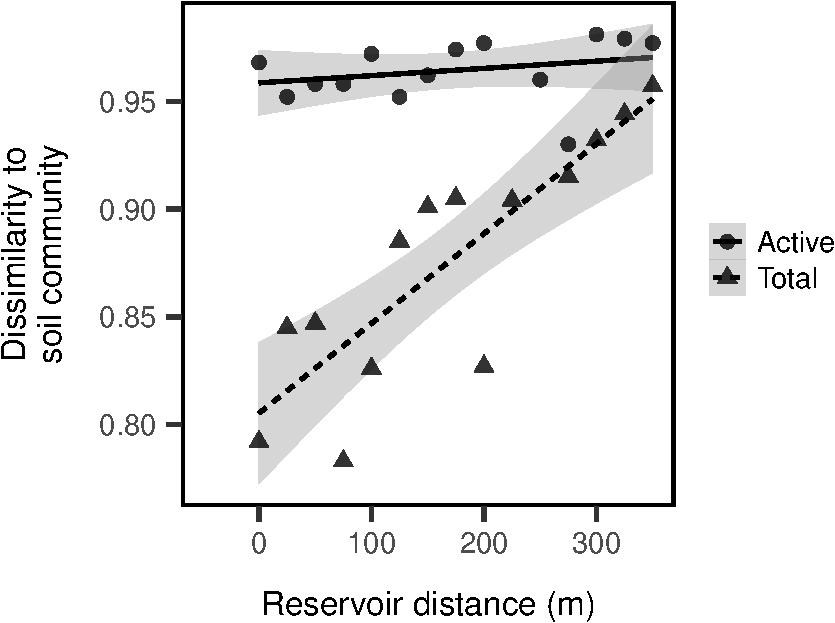
\includegraphics{ReservoirGradient_files/figure-latex/unnamed-chunk-3-1} \end{center}

\begin{Shaded}
\begin{Highlighting}[]
\NormalTok{betadivcomp.sor <-}\StringTok{ }\KeywordTok{beta.div.comp}\NormalTok{(}\DataTypeTok{mat =}\NormalTok{ OTUsREL.log, }\DataTypeTok{coef =} \StringTok{"S"}\NormalTok{, }\DataTypeTok{quant =} \OtherTok{FALSE}\NormalTok{, }\DataTypeTok{save.abc =} \OtherTok{FALSE}\NormalTok{)}

\NormalTok{rich.lake <-}\StringTok{ }\KeywordTok{as.matrix}\NormalTok{(betadivcomp.sor}\OperatorTok{$}\NormalTok{rich)[}\OperatorTok{-}\KeywordTok{c}\NormalTok{(}\DecValTok{1}\OperatorTok{:}\DecValTok{3}\NormalTok{), }\DecValTok{1}\OperatorTok{:}\DecValTok{3}\NormalTok{] }
\NormalTok{rich.se      <-}\StringTok{ }\KeywordTok{round}\NormalTok{(}\KeywordTok{apply}\NormalTok{(rich.lake, }\DecValTok{1}\NormalTok{, se), }\DecValTok{3}\NormalTok{)}
\NormalTok{rich.mean    <-}\StringTok{ }\KeywordTok{round}\NormalTok{(}\KeywordTok{apply}\NormalTok{(rich.lake, }\DecValTok{1}\NormalTok{, mean), }\DecValTok{3}\NormalTok{)}
\NormalTok{UL.rich       <-}\StringTok{ }\KeywordTok{cbind}\NormalTok{(design[}\OperatorTok{-}\KeywordTok{c}\NormalTok{(}\DecValTok{1}\OperatorTok{:}\DecValTok{3}\NormalTok{), ], rich.mean, rich.se)}

\NormalTok{repl.lake <-}\StringTok{ }\KeywordTok{as.matrix}\NormalTok{(betadivcomp.sor}\OperatorTok{$}\NormalTok{repl)[}\OperatorTok{-}\KeywordTok{c}\NormalTok{(}\DecValTok{1}\OperatorTok{:}\DecValTok{3}\NormalTok{), }\DecValTok{1}\OperatorTok{:}\DecValTok{3}\NormalTok{] }
\NormalTok{repl.mean    <-}\StringTok{ }\KeywordTok{round}\NormalTok{(}\KeywordTok{apply}\NormalTok{(repl.lake, }\DecValTok{1}\NormalTok{, mean), }\DecValTok{3}\NormalTok{)}
\NormalTok{repl.se      <-}\StringTok{ }\KeywordTok{round}\NormalTok{(}\KeywordTok{apply}\NormalTok{(repl.lake, }\DecValTok{1}\NormalTok{, se), }\DecValTok{3}\NormalTok{)}
\NormalTok{UL.repl       <-}\StringTok{ }\KeywordTok{cbind}\NormalTok{(design[}\OperatorTok{-}\KeywordTok{c}\NormalTok{(}\DecValTok{1}\OperatorTok{:}\DecValTok{3}\NormalTok{), ], repl.mean, repl.se)}

\NormalTok{UL_betapartitions <-}\StringTok{ }\KeywordTok{left_join}\NormalTok{(UL.nest, UL.turn) }\OperatorTok\StringTok{ }\KeywordTok{left_join}\NormalTok{(UL.rich) }\OperatorTok\StringTok{ }\KeywordTok{left_join}\NormalTok{(UL.repl) }\OperatorTok\StringTok{ }
\StringTok{  }\KeywordTok{gather}\NormalTok{(nest.se, turn.se, rich.se, repl.se, }\DataTypeTok{key =} \StringTok{"partition"}\NormalTok{, }\DataTypeTok{value =} \StringTok{"se"}\NormalTok{) }\OperatorTok\StringTok{ }
\StringTok{  }\KeywordTok{gather}\NormalTok{(nest.mean, turn.mean, rich.mean, repl.mean, }\DataTypeTok{key =} \StringTok{"partition"}\NormalTok{, }\DataTypeTok{value =} \StringTok{"beta"}\NormalTok{)}
  
\NormalTok{UL_betapartitions }\OperatorTok\StringTok{ }
\StringTok{  }\KeywordTok{mutate}\NormalTok{(}\DataTypeTok{molecule =} \KeywordTok{ifelse}\NormalTok{(molecule }\OperatorTok{==}\StringTok{ "DNA"}\NormalTok{, }\StringTok{"Total"}\NormalTok{, }\StringTok{"Active"}\NormalTok{)) }\OperatorTok\StringTok{ }
\StringTok{  }\KeywordTok{mutate}\NormalTok{(}\DataTypeTok{family =} \KeywordTok{ifelse}\NormalTok{(partition }\OperatorTok\StringTok{ }\KeywordTok{c}\NormalTok{(}\StringTok{"nest.mean"}\NormalTok{, }\StringTok{"turn.mean"}\NormalTok{), }\StringTok{"Baselga"}\NormalTok{, }\StringTok{"Podani"}\NormalTok{)) }\OperatorTok\StringTok{ }
\StringTok{  }\KeywordTok{filter}\NormalTok{(family }\OperatorTok{==}\StringTok{ "Baselga"}\NormalTok{) }\OperatorTok\StringTok{ }
\StringTok{  }\KeywordTok{mutate}\NormalTok{(}\DataTypeTok{partition =} \KeywordTok{ifelse}\NormalTok{(partition }\OperatorTok{==}\StringTok{ "nest.mean"}\NormalTok{, }\StringTok{"Mean Nestedness"}\NormalTok{, }\StringTok{"Mean Turnover"}\NormalTok{)) }\OperatorTok\StringTok{ }
\StringTok{  }\KeywordTok{ggplot}\NormalTok{(}\KeywordTok{aes}\NormalTok{(}\DataTypeTok{x =}\NormalTok{ distance, }\DataTypeTok{y =}\NormalTok{ beta, }\DataTypeTok{shape =}\NormalTok{ molecule)) }\OperatorTok{+}
\StringTok{  }\KeywordTok{geom_smooth}\NormalTok{(}\DataTypeTok{method =} \StringTok{"lm"}\NormalTok{, }\KeywordTok{aes}\NormalTok{(}\DataTypeTok{linetype =}\NormalTok{ molecule), }\DataTypeTok{color =} \StringTok{"black"}\NormalTok{, }\DataTypeTok{show.legend =}\NormalTok{ T) }\OperatorTok{+}\StringTok{ }
\StringTok{  }\KeywordTok{geom_point}\NormalTok{(}\DataTypeTok{alpha =} \FloatTok{0.3}\NormalTok{, }\DataTypeTok{size =} \DecValTok{3}\NormalTok{, }\DataTypeTok{show.legend =}\NormalTok{ T) }\OperatorTok{+}\StringTok{ }
\StringTok{  }\CommentTok{#geom_errorbar(aes(ymax = beta + se, ymin = beta - se), width = 10) +}
\StringTok{  }\KeywordTok{facet_wrap}\NormalTok{(.}\OperatorTok{~}\NormalTok{partition) }\OperatorTok{+}
\StringTok{  }\KeywordTok{labs}\NormalTok{(}\DataTypeTok{y =} \KeywordTok{str_wrap}\NormalTok{(}\StringTok{"Beta diversity partition (Sorensen)"}\NormalTok{, }\DataTypeTok{width =} \DecValTok{20}\NormalTok{), }
       \DataTypeTok{x =} \StringTok{"Reservoir distance (m)"}\NormalTok{) }\OperatorTok{+}\StringTok{ }
\StringTok{  }\KeywordTok{scale_x_continuous}\NormalTok{(}\DataTypeTok{limits =} \KeywordTok{c}\NormalTok{(}\OperatorTok{-}\DecValTok{49}\NormalTok{,}\DecValTok{350}\NormalTok{)) }\OperatorTok{+}
\StringTok{  }\KeywordTok{ggsave}\NormalTok{(}\StringTok{"figures/FigureS3.pdf"}\NormalTok{, }\DataTypeTok{width =} \DecValTok{8}\NormalTok{, }\DataTypeTok{height =} \DecValTok{4}\NormalTok{)}
\end{Highlighting}
\end{Shaded}

\begin{center}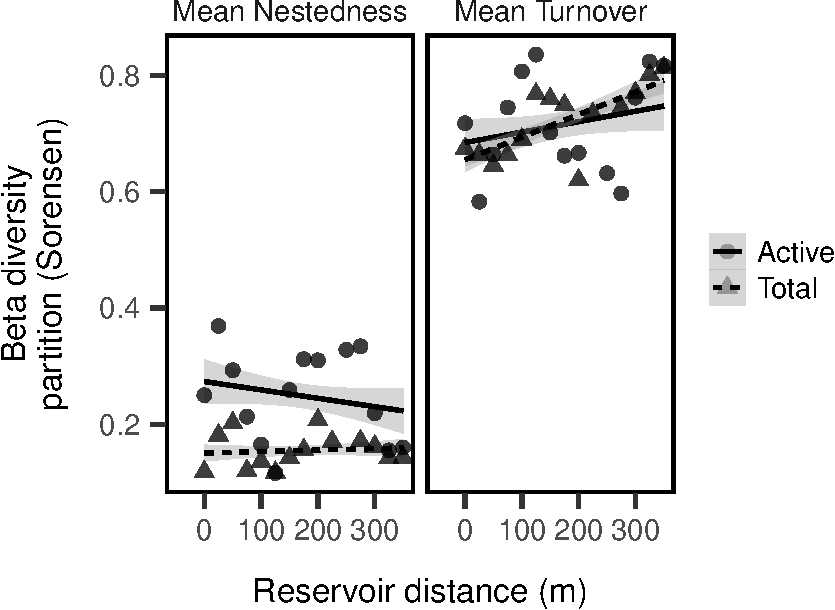
\includegraphics{ReservoirGradient_files/figure-latex/unnamed-chunk-3-2} \end{center}

\hypertarget{identifying-the-soil-bacteria}{%
\section{Identifying the Soil
Bacteria}\label{identifying-the-soil-bacteria}}

Now, we wish to determine whether soil-derived taxa are driving this
pattern, and then ask who these influential soil bacteria are.

To classify soil bacteria, we take an incidence-based approach and
classify OTUs as:\\
- present in the soil and present, but never active, in the reservoir\\
- present in the soil and active in the reservoir

\begin{Shaded}
\begin{Highlighting}[]
\CommentTok{# separate lake and soil samples}
\NormalTok{lake.total <-}\StringTok{ }\NormalTok{OTUs[}\KeywordTok{which}\NormalTok{(design}\OperatorTok{$}\NormalTok{molecule }\OperatorTok{==}\StringTok{ "DNA"}\NormalTok{, design}\OperatorTok{$}\NormalTok{type }\OperatorTok{==}\StringTok{ "water"}\NormalTok{),]}
\NormalTok{soil.total <-}\StringTok{ }\NormalTok{OTUs[}\KeywordTok{which}\NormalTok{(design}\OperatorTok{$}\NormalTok{molecule }\OperatorTok{==}\StringTok{ "DNA"}\NormalTok{, design}\OperatorTok{$}\NormalTok{type }\OperatorTok{==}\StringTok{ "soil"}\NormalTok{),]}

\CommentTok{# which otus are present in both lake and soil samples}
\NormalTok{lake.and.soil.total <-}\StringTok{ }\NormalTok{OTUs[}\KeywordTok{which}\NormalTok{(design}\OperatorTok{$}\NormalTok{molecule }\OperatorTok{==}\StringTok{ "DNA"}\NormalTok{, design}\OperatorTok{$}\NormalTok{type }\OperatorTok{==}\StringTok{ "water"}\NormalTok{),}
                            \KeywordTok{which}\NormalTok{(}\KeywordTok{colSums}\NormalTok{(lake.total) }\OperatorTok{>}\StringTok{ }\DecValTok{0} \OperatorTok{&}\StringTok{ }\KeywordTok{colSums}\NormalTok{(soil.total) }\OperatorTok{>}\StringTok{ }\DecValTok{0}\NormalTok{)]}

\CommentTok{# isolate just the dna and rna lake communities}
\NormalTok{w.dna <-}\StringTok{ }\NormalTok{OTUs[}\KeywordTok{which}\NormalTok{(design}\OperatorTok{$}\NormalTok{molecule }\OperatorTok{==}\StringTok{ "DNA"} \OperatorTok{&}\StringTok{ }\NormalTok{design}\OperatorTok{$}\NormalTok{type }\OperatorTok{==}\StringTok{ "water"}\NormalTok{), ]}
\NormalTok{w.rna <-}\StringTok{ }\NormalTok{OTUs[}\KeywordTok{which}\NormalTok{(design}\OperatorTok{$}\NormalTok{molecule }\OperatorTok{==}\StringTok{ "RNA"} \OperatorTok{&}\StringTok{ }\NormalTok{design}\OperatorTok{$}\NormalTok{type }\OperatorTok{==}\StringTok{ "water"}\NormalTok{), ]}

\CommentTok{# pull out the lake rna counts for otus found in lake and soil}
\NormalTok{lake.and.soil.act <-}\StringTok{ }\NormalTok{w.rna[,}\KeywordTok{colnames}\NormalTok{(lake.and.soil.total)]}

\CommentTok{# of these lake and soil taxa, which are never active? active?}
\NormalTok{nvr.act <-}\StringTok{ }\KeywordTok{which}\NormalTok{(}\KeywordTok{colSums}\NormalTok{(lake.and.soil.act) }\OperatorTok{==}\StringTok{ }\DecValTok{0}\NormalTok{)}
\NormalTok{yes.act <-}\StringTok{ }\KeywordTok{which}\NormalTok{(}\KeywordTok{colSums}\NormalTok{(lake.and.soil.act) }\OperatorTok{!=}\StringTok{ }\DecValTok{0}\NormalTok{)}

\CommentTok{# how many otus are active relative to the total number of otus }
\KeywordTok{length}\NormalTok{(nvr.act) }\OperatorTok{/}\StringTok{ }\KeywordTok{ncol}\NormalTok{(lake.and.soil.total) }\CommentTok{# 88% of soil-derived bac never active}
\end{Highlighting}
\end{Shaded}

\begin{verbatim}
## [1] 0.8210454
\end{verbatim}

\begin{Shaded}
\begin{Highlighting}[]
\KeywordTok{length}\NormalTok{(yes.act) }\OperatorTok{/}\StringTok{ }\KeywordTok{ncol}\NormalTok{(soil.total) }\CommentTok{# 8% of all soil taxa were active in lake}
\end{Highlighting}
\end{Shaded}

\begin{verbatim}
## [1] 0.1327096
\end{verbatim}

\begin{Shaded}
\begin{Highlighting}[]
\CommentTok{# of taxa who were never active, what fraction of the total community did they represent?}
\KeywordTok{sum}\NormalTok{(}\KeywordTok{rowSums}\NormalTok{(w.dna[,}\KeywordTok{names}\NormalTok{(nvr.act)]))}
\end{Highlighting}
\end{Shaded}

\begin{verbatim}
## [1] 23585
\end{verbatim}

\begin{Shaded}
\begin{Highlighting}[]
\KeywordTok{sum}\NormalTok{(}\KeywordTok{rowSums}\NormalTok{(w.dna[,}\KeywordTok{names}\NormalTok{(yes.act)]))}
\end{Highlighting}
\end{Shaded}

\begin{verbatim}
## [1] 499388
\end{verbatim}

\begin{Shaded}
\begin{Highlighting}[]
\KeywordTok{sum}\NormalTok{(}\KeywordTok{rowSums}\NormalTok{(w.dna[,}\KeywordTok{names}\NormalTok{(nvr.act)])) }\OperatorTok{/}\StringTok{ }\KeywordTok{sum}\NormalTok{(}\KeywordTok{rowSums}\NormalTok{(w.dna))}
\end{Highlighting}
\end{Shaded}

\begin{verbatim}
## [1] 0.04509793
\end{verbatim}

\begin{Shaded}
\begin{Highlighting}[]
\CommentTok{# of taxa who became active, what fraction of the dna community did they represent?}
\KeywordTok{sum}\NormalTok{(}\KeywordTok{rowSums}\NormalTok{(w.dna[,}\KeywordTok{names}\NormalTok{(yes.act)])) }\OperatorTok{/}\StringTok{ }\KeywordTok{sum}\NormalTok{(}\KeywordTok{rowSums}\NormalTok{(w.dna))}
\end{Highlighting}
\end{Shaded}

\begin{verbatim}
## [1] 0.9549021
\end{verbatim}

\begin{Shaded}
\begin{Highlighting}[]
\NormalTok{prop.nvr.act <-}\StringTok{ }\KeywordTok{rowSums}\NormalTok{(w.dna[,nvr.act]) }\OperatorTok{/}\StringTok{ }\KeywordTok{rowSums}\NormalTok{(w.dna)}
\CommentTok{# cbind.data.frame(design.dna, inactive = prop.nvr.act) %>% }
\CommentTok{#   ggplot(aes(x = distance, y = inactive)) +}
\CommentTok{#   geom_point() + }
\CommentTok{#   geom_line(stat = "smooth", method = "lm", formula = y ~ x, se = F) +}
\CommentTok{#   labs(x = "Reservoir transect (m)", y = "Rel. abundance of taxa\textbackslash{}n that are never active") +}
\CommentTok{#   scale_x_reverse()}
\end{Highlighting}
\end{Shaded}

We calculate the richness of the soil taxa that are never active in the
lake. We calculate richness from the DNA-based samples.

\begin{Shaded}
\begin{Highlighting}[]
\CommentTok{# pull out their dna abundances and calculate richness}
\NormalTok{terr.lake <-}\StringTok{ }\NormalTok{w.dna[ , }\KeywordTok{c}\NormalTok{(}\KeywordTok{names}\NormalTok{(nvr.act))]}
\NormalTok{terr.rich <-}\StringTok{ }\KeywordTok{rowSums}\NormalTok{((terr.lake }\OperatorTok{>}\StringTok{ }\DecValTok{0}\NormalTok{) }\OperatorTok{*}\StringTok{ }\DecValTok{1}\NormalTok{)}
\NormalTok{terr.REL <-}\StringTok{ }\KeywordTok{rowSums}\NormalTok{(terr.lake) }\OperatorTok{/}\StringTok{ }\KeywordTok{rowSums}\NormalTok{(w.dna) }
\NormalTok{design.dna <-}\StringTok{ }\NormalTok{design[}\KeywordTok{which}\NormalTok{(design}\OperatorTok{$}\NormalTok{molecule }\OperatorTok{==}\StringTok{ "DNA"} \OperatorTok{&}\StringTok{ }\NormalTok{design}\OperatorTok{$}\NormalTok{type }\OperatorTok{==}\StringTok{ "water"}\NormalTok{), ]}
\NormalTok{terr.rich.log <-}\StringTok{ }\KeywordTok{log10}\NormalTok{(terr.rich)}
\NormalTok{terr.REL.log <-}\StringTok{ }\KeywordTok{log10}\NormalTok{(terr.REL)}

\NormalTok{terr.mod1 <-}\StringTok{ }\KeywordTok{lm}\NormalTok{(terr.rich.log }\OperatorTok{~}\StringTok{ }\NormalTok{design.dna}\OperatorTok{$}\NormalTok{distance)}
\KeywordTok{summary}\NormalTok{(terr.mod1)}
\end{Highlighting}
\end{Shaded}

\begin{verbatim}
## 
## Call:
## lm(formula = terr.rich.log ~ design.dna$distance)
## 
## Residuals:
##       Min        1Q    Median        3Q       Max 
## -0.199417 -0.123300 -0.000783  0.080926  0.234711 
## 
## Coefficients:
##                       Estimate Std. Error t value Pr(>|t|)    
## (Intercept)          3.0266909  0.0726577  41.657 2.37e-14 ***
## design.dna$distance -0.0025661  0.0003595  -7.138 1.18e-05 ***
## ---
## Signif. codes:  0 '***' 0.001 '**' 0.01 '*' 0.05 '.' 0.1 ' ' 1
## 
## Residual standard error: 0.1478 on 12 degrees of freedom
## Multiple R-squared:  0.8094, Adjusted R-squared:  0.7935 
## F-statistic: 50.95 on 1 and 12 DF,  p-value: 1.184e-05
\end{verbatim}

\begin{Shaded}
\begin{Highlighting}[]
\NormalTok{T1.R2 <-}\StringTok{ }\KeywordTok{round}\NormalTok{(}\KeywordTok{summary}\NormalTok{(terr.mod1)}\OperatorTok{$}\NormalTok{r.squared, }\DecValTok{2}\NormalTok{)}
\NormalTok{T1.int <-}\StringTok{ }\NormalTok{terr.mod1}\OperatorTok{$}\NormalTok{coefficients[}\DecValTok{1}\NormalTok{]}
\NormalTok{T1.slp <-}\StringTok{ }\NormalTok{terr.mod1}\OperatorTok{$}\NormalTok{coefficients[}\DecValTok{2}\NormalTok{]}
\KeywordTok{pander}\NormalTok{(terr.mod1)}
\end{Highlighting}
\end{Shaded}

\begin{longtable}[]{@{}ccccc@{}}
\caption{Fitting linear model: terr.rich.log \textasciitilde{}
design.dna\$distance We find distance is a highly significant predictor
of the richness of these soil-derived taxa (on a
log-scale).}\tabularnewline
\toprule
\begin{minipage}[b]{0.31\columnwidth}\centering
~\strut
\end{minipage} & \begin{minipage}[b]{0.14\columnwidth}\centering
Estimate\strut
\end{minipage} & \begin{minipage}[b]{0.15\columnwidth}\centering
Std. Error\strut
\end{minipage} & \begin{minipage}[b]{0.12\columnwidth}\centering
t value\strut
\end{minipage} & \begin{minipage}[b]{0.14\columnwidth}\centering
Pr(\textgreater{}\textbar{}t\textbar{})\strut
\end{minipage}\tabularnewline
\midrule
\endfirsthead
\toprule
\begin{minipage}[b]{0.31\columnwidth}\centering
~\strut
\end{minipage} & \begin{minipage}[b]{0.14\columnwidth}\centering
Estimate\strut
\end{minipage} & \begin{minipage}[b]{0.15\columnwidth}\centering
Std. Error\strut
\end{minipage} & \begin{minipage}[b]{0.12\columnwidth}\centering
t value\strut
\end{minipage} & \begin{minipage}[b]{0.14\columnwidth}\centering
Pr(\textgreater{}\textbar{}t\textbar{})\strut
\end{minipage}\tabularnewline
\midrule
\endhead
\begin{minipage}[t]{0.31\columnwidth}\centering
\textbf{(Intercept)}\strut
\end{minipage} & \begin{minipage}[t]{0.14\columnwidth}\centering
3.027\strut
\end{minipage} & \begin{minipage}[t]{0.15\columnwidth}\centering
0.07266\strut
\end{minipage} & \begin{minipage}[t]{0.12\columnwidth}\centering
41.66\strut
\end{minipage} & \begin{minipage}[t]{0.14\columnwidth}\centering
2.374e-14\strut
\end{minipage}\tabularnewline
\begin{minipage}[t]{0.31\columnwidth}\centering
\textbf{design.dna\$distance}\strut
\end{minipage} & \begin{minipage}[t]{0.14\columnwidth}\centering
-0.002566\strut
\end{minipage} & \begin{minipage}[t]{0.15\columnwidth}\centering
0.0003595\strut
\end{minipage} & \begin{minipage}[t]{0.12\columnwidth}\centering
-7.138\strut
\end{minipage} & \begin{minipage}[t]{0.14\columnwidth}\centering
1.184e-05\strut
\end{minipage}\tabularnewline
\bottomrule
\end{longtable}

\hypertarget{figure-3-fate-of-terrestrial-bacteria}{%
\section{Figure 3: Fate of terrestrial
bacteria}\label{figure-3-fate-of-terrestrial-bacteria}}

\hypertarget{panel-3a-transients}{%
\subsection{Panel 3a: transients}\label{panel-3a-transients}}

\begin{Shaded}
\begin{Highlighting}[]
\NormalTok{transient.plot <-}\StringTok{ }\KeywordTok{tibble}\NormalTok{(}\DataTypeTok{transient_rich =}\NormalTok{ terr.rich, }\DataTypeTok{distance =}\NormalTok{ design.dna}\OperatorTok{$}\NormalTok{distance) }\OperatorTok\StringTok{ }
\StringTok{  }\KeywordTok{ggplot}\NormalTok{(}\KeywordTok{aes}\NormalTok{(}\DataTypeTok{x =}\NormalTok{ distance, }\DataTypeTok{y =}\NormalTok{ transient_rich)) }\OperatorTok{+}\StringTok{ }
\StringTok{  }\KeywordTok{geom_smooth}\NormalTok{(}\DataTypeTok{method =} \StringTok{"lm"}\NormalTok{, }\DataTypeTok{color =} \StringTok{"black"}\NormalTok{, }\DataTypeTok{fill =} \StringTok{"grey"}\NormalTok{) }\OperatorTok{+}
\StringTok{  }\KeywordTok{geom_point}\NormalTok{(}\DataTypeTok{size =} \DecValTok{3}\NormalTok{, }\DataTypeTok{alpha =} \FloatTok{.8}\NormalTok{, }\DataTypeTok{color =} \StringTok{"black"}\NormalTok{) }\OperatorTok{+}\StringTok{ }
\StringTok{  }\KeywordTok{scale_y_log10}\NormalTok{() }\OperatorTok{+}
\StringTok{  }\KeywordTok{annotation_logticks}\NormalTok{(}\DataTypeTok{sides =} \StringTok{"l"}\NormalTok{, }\DataTypeTok{size =} \DecValTok{1}\NormalTok{) }\OperatorTok{+}
\StringTok{  }\KeywordTok{labs}\NormalTok{(}\DataTypeTok{x =} \StringTok{"Reservoir distance (m)"}\NormalTok{,}
       \DataTypeTok{y =} \StringTok{"Inactive soil taxa in reservoir"}\NormalTok{) }\OperatorTok{+}
\StringTok{  }\KeywordTok{annotate}\NormalTok{(}\StringTok{"text"}\NormalTok{, }\DataTypeTok{x =} \DecValTok{350}\NormalTok{, }\DataTypeTok{y =} \KeywordTok{max}\NormalTok{(terr.rich) }\OperatorTok{+}\StringTok{ }\DecValTok{200}\NormalTok{, }\DataTypeTok{hjust =} \DecValTok{1}\NormalTok{, }\DataTypeTok{vjust =} \DecValTok{0}\NormalTok{, }\DataTypeTok{size =} \DecValTok{5}\NormalTok{,}
           \DataTypeTok{label =} \KeywordTok{paste0}\NormalTok{(}\StringTok{"r^2== "}\NormalTok{,T1.R2), }\DataTypeTok{parse =}\NormalTok{ T)}
\end{Highlighting}
\end{Shaded}

\hypertarget{what-is-the-fate-of-soil-derived-taxa-in-the-reservoir}{%
\subsection{What is the fate of soil-derived taxa in the
reservoir?}\label{what-is-the-fate-of-soil-derived-taxa-in-the-reservoir}}

So, we observe that most soil-derived taxa appear to decay once they
enter the reservoir. Do any soil-derived taxa persist in the active
bacterial community of the reservoir and do they rise to high relative
abundances?

\begin{Shaded}
\begin{Highlighting}[]
\CommentTok{# identify otus in soil samples and lake samples}
\NormalTok{in.soil <-}\StringTok{ }\NormalTok{OTUs[, }\KeywordTok{which}\NormalTok{(}\KeywordTok{colSums}\NormalTok{(OTUs[}\KeywordTok{c}\NormalTok{(}\DecValTok{1}\OperatorTok{:}\DecValTok{3}\NormalTok{),]) }\OperatorTok{>}\StringTok{ }\DecValTok{0}\NormalTok{ )]}
\CommentTok{#in.lake <- OTUs[, which(colSums(OTUs[-c(1:3),]) > 0)]}

\CommentTok{# isolate just the rna water samples and convert to presence-absence}
\NormalTok{in.lake.rna <-}\StringTok{ }\NormalTok{OTUs[}\KeywordTok{which}\NormalTok{(design}\OperatorTok{$}\NormalTok{molecule }\OperatorTok{==}\StringTok{ "RNA"} \OperatorTok{&}\StringTok{ }\NormalTok{design}\OperatorTok{$}\NormalTok{type }\OperatorTok{==}\StringTok{ "water"}\NormalTok{), ]}
\NormalTok{in.lake.rna.pa <-}\StringTok{ }\NormalTok{(in.lake.rna }\OperatorTok{>}\StringTok{ }\DecValTok{0}\NormalTok{) }\OperatorTok{*}\StringTok{ }\DecValTok{1}

\CommentTok{# define the 'core' taxa as otus present in 50% of samples}
\NormalTok{in.lake.core <-}\StringTok{ }\NormalTok{w.dna[, }\KeywordTok{which}\NormalTok{((}\KeywordTok{colSums}\NormalTok{(in.lake.rna.pa) }\OperatorTok{/}\StringTok{ }\KeywordTok{nrow}\NormalTok{(in.lake.rna.pa)) }\OperatorTok{>=}\StringTok{ }\FloatTok{0.75}\NormalTok{)]}

\CommentTok{# of the core, how many are also in the soil samples?}
\NormalTok{in.lake.core.from.soils <-}\StringTok{ }\NormalTok{in.lake.core[, }\KeywordTok{intersect}\NormalTok{(}\KeywordTok{colnames}\NormalTok{(in.lake.core), }\KeywordTok{colnames}\NormalTok{(in.soil))]}

\CommentTok{# of the core which are not in the soil samples}
\NormalTok{in.lake.core.not.soils <-}\StringTok{ }\NormalTok{in.lake.core[, }\KeywordTok{setdiff}\NormalTok{(}\KeywordTok{colnames}\NormalTok{(in.lake.core), }\KeywordTok{colnames}\NormalTok{(in.soil))]}

\CommentTok{# Find the relative abundance of the core taxa and prepare data frame to plot}
\NormalTok{in.lake.core.from.soils.REL <-}\StringTok{ }\NormalTok{in.lake.core.from.soils }\OperatorTok{/}\StringTok{ }\KeywordTok{rowSums}\NormalTok{(w.dna)}

\NormalTok{in.soil.to.plot <-}\StringTok{ }\KeywordTok{as.data.frame}\NormalTok{(in.lake.core.from.soils.REL) }\OperatorTok\StringTok{ }
\StringTok{  }\KeywordTok{rownames_to_column}\NormalTok{(}\StringTok{"sample_ID"}\NormalTok{) }\OperatorTok\StringTok{ }
\StringTok{  }\KeywordTok{gather}\NormalTok{(otu_id, rel_abundance, }\OperatorTok{-}\NormalTok{sample_ID) }\OperatorTok\StringTok{ }
\StringTok{  }\KeywordTok{left_join}\NormalTok{(}\KeywordTok{rownames_to_column}\NormalTok{(design.dna, }\StringTok{"sample_ID"}\NormalTok{)) }\OperatorTok\StringTok{ }
\StringTok{  }\KeywordTok{add_column}\NormalTok{(}\DataTypeTok{found =} \StringTok{"soils"}\NormalTok{)}

\NormalTok{in.lake.core.not.soils.REL <-}\StringTok{ }\NormalTok{in.lake.core.not.soils }\OperatorTok{/}\StringTok{ }\KeywordTok{rowSums}\NormalTok{(w.dna)}

\NormalTok{in.lake.to.plot <-}\StringTok{ }\KeywordTok{as.data.frame}\NormalTok{(in.lake.core.not.soils.REL) }\OperatorTok\StringTok{ }
\StringTok{  }\KeywordTok{rownames_to_column}\NormalTok{(}\StringTok{"sample_ID"}\NormalTok{) }\OperatorTok\StringTok{ }
\StringTok{  }\KeywordTok{gather}\NormalTok{(otu_id, rel_abundance, }\OperatorTok{-}\NormalTok{sample_ID) }\OperatorTok\StringTok{ }
\StringTok{  }\KeywordTok{left_join}\NormalTok{(}\KeywordTok{rownames_to_column}\NormalTok{(design.dna, }\StringTok{"sample_ID"}\NormalTok{)) }\OperatorTok\StringTok{ }
\StringTok{  }\KeywordTok{add_column}\NormalTok{(}\DataTypeTok{found =} \StringTok{"lake"}\NormalTok{)}
\end{Highlighting}
\end{Shaded}

\begin{Shaded}
\begin{Highlighting}[]
\CommentTok{# model distance effect on rel abundance to get slope and pval}
\NormalTok{soil.core.mods <-}\StringTok{ }\KeywordTok{apply}\NormalTok{(in.lake.core.from.soils.REL, }\DataTypeTok{MARGIN =} \DecValTok{2}\NormalTok{, }
    \DataTypeTok{FUN =} \ControlFlowTok{function}\NormalTok{(x) }\KeywordTok{summary}\NormalTok{(}\KeywordTok{lm}\NormalTok{(x }\OperatorTok{~}\StringTok{ }\NormalTok{design.dna}\OperatorTok{$}\NormalTok{distance))}\OperatorTok{$}\NormalTok{coefficients[}\DecValTok{2}\NormalTok{,}\KeywordTok{c}\NormalTok{(}\DecValTok{1}\NormalTok{,}\DecValTok{4}\NormalTok{)])}
\KeywordTok{rownames}\NormalTok{(soil.core.mods) <-}\StringTok{ }\KeywordTok{c}\NormalTok{(}\StringTok{"slope"}\NormalTok{, }\StringTok{"pval"}\NormalTok{)}

\CommentTok{# classify otus as significantly increasing or decreasing along reservoir}
\NormalTok{soil.core.decreasing <-}\StringTok{ }\KeywordTok{as.data.frame}\NormalTok{(}\KeywordTok{t}\NormalTok{(soil.core.mods)) }\OperatorTok\StringTok{ }
\StringTok{  }\KeywordTok{rownames_to_column}\NormalTok{(}\StringTok{"OTU"}\NormalTok{) }\OperatorTok\StringTok{ }
\StringTok{  }\KeywordTok{filter}\NormalTok{(slope }\OperatorTok{<}\StringTok{ }\DecValTok{0}\NormalTok{) }\OperatorTok\StringTok{   }\CommentTok{# rel abund decreases toward dam}
\StringTok{  }\KeywordTok{left_join}\NormalTok{(OTU.tax)}
\end{Highlighting}
\end{Shaded}

\begin{verbatim}
## Warning: Column `OTU` joining character vector and factor, coercing into
## character vector
\end{verbatim}

\begin{Shaded}
\begin{Highlighting}[]
\NormalTok{soil.core.increasing <-}\StringTok{ }\KeywordTok{as.data.frame}\NormalTok{(}\KeywordTok{t}\NormalTok{(soil.core.mods)) }\OperatorTok\StringTok{ }
\StringTok{  }\KeywordTok{rownames_to_column}\NormalTok{(}\StringTok{"OTU"}\NormalTok{) }\OperatorTok\StringTok{ }
\StringTok{  }\KeywordTok{filter}\NormalTok{(slope }\OperatorTok{>}\StringTok{ }\DecValTok{0}\NormalTok{) }\OperatorTok\StringTok{   }\CommentTok{# rel abund increases toward dam}
\StringTok{  }\KeywordTok{left_join}\NormalTok{(OTU.tax)}
\end{Highlighting}
\end{Shaded}

\begin{verbatim}
## Warning: Column `OTU` joining character vector and factor, coercing into
## character vector
\end{verbatim}

\begin{Shaded}
\begin{Highlighting}[]
\NormalTok{nonsoil.core.mods <-}\StringTok{ }\KeywordTok{apply}\NormalTok{(in.lake.core.not.soils.REL, }\DataTypeTok{MARGIN =} \DecValTok{2}\NormalTok{, }
    \DataTypeTok{FUN =} \ControlFlowTok{function}\NormalTok{(x) }\KeywordTok{summary}\NormalTok{(}\KeywordTok{lm}\NormalTok{(x }\OperatorTok{~}\StringTok{ }\NormalTok{design.dna}\OperatorTok{$}\NormalTok{distance))}\OperatorTok{$}\NormalTok{coefficients[}\DecValTok{2}\NormalTok{,}\KeywordTok{c}\NormalTok{(}\DecValTok{1}\NormalTok{,}\DecValTok{4}\NormalTok{)])}
\KeywordTok{rownames}\NormalTok{(nonsoil.core.mods) <-}\StringTok{ }\KeywordTok{c}\NormalTok{(}\StringTok{"slope"}\NormalTok{, }\StringTok{"pval"}\NormalTok{)}
\NormalTok{nonsoil.core.decreasing <-}\StringTok{ }\KeywordTok{as.data.frame}\NormalTok{(}\KeywordTok{t}\NormalTok{(nonsoil.core.mods)) }\OperatorTok\StringTok{ }
\StringTok{  }\KeywordTok{rownames_to_column}\NormalTok{(}\StringTok{"OTU"}\NormalTok{) }\OperatorTok\StringTok{ }
\StringTok{  }\KeywordTok{filter}\NormalTok{(slope }\OperatorTok{<}\StringTok{ }\DecValTok{0}\NormalTok{) }\OperatorTok\StringTok{   }\CommentTok{# rel abund decreases toward dam}
\StringTok{  }\KeywordTok{left_join}\NormalTok{(OTU.tax)}
\end{Highlighting}
\end{Shaded}

\begin{verbatim}
## Warning: Column `OTU` joining character vector and factor, coercing into
## character vector
\end{verbatim}

\begin{Shaded}
\begin{Highlighting}[]
\NormalTok{nonsoil.core.increasing <-}\StringTok{ }\KeywordTok{as.data.frame}\NormalTok{(}\KeywordTok{t}\NormalTok{(nonsoil.core.mods)) }\OperatorTok\StringTok{ }
\StringTok{  }\KeywordTok{rownames_to_column}\NormalTok{(}\StringTok{"OTU"}\NormalTok{) }\OperatorTok\StringTok{ }
\StringTok{  }\KeywordTok{filter}\NormalTok{(slope }\OperatorTok{>}\StringTok{ }\DecValTok{0}\NormalTok{) }\OperatorTok\StringTok{   }\CommentTok{# rel abund increases toward dam}
\StringTok{  }\KeywordTok{left_join}\NormalTok{(OTU.tax)}
\end{Highlighting}
\end{Shaded}

\begin{verbatim}
## Warning: Column `OTU` joining character vector and factor, coercing into
## character vector
\end{verbatim}

\hypertarget{table-s1-and-s2}{%
\subsection{Table S1 and S2}\label{table-s1-and-s2}}

\begin{Shaded}
\begin{Highlighting}[]
\KeywordTok{pander}\NormalTok{(soil.core.decreasing, }\DataTypeTok{caption =} \StringTok{"Core taxa found in soils that get rarer along the transect."}\NormalTok{)}
\end{Highlighting}
\end{Shaded}

\begin{longtable}[]{@{}ccccc@{}}
\caption{Core taxa found in soils that get rarer along the transect.
(continued below)}\tabularnewline
\toprule
\begin{minipage}[b]{0.13\columnwidth}\centering
OTU\strut
\end{minipage} & \begin{minipage}[b]{0.16\columnwidth}\centering
slope\strut
\end{minipage} & \begin{minipage}[b]{0.12\columnwidth}\centering
pval\strut
\end{minipage} & \begin{minipage}[b]{0.13\columnwidth}\centering
Domain\strut
\end{minipage} & \begin{minipage}[b]{0.21\columnwidth}\centering
Phylum\strut
\end{minipage}\tabularnewline
\midrule
\endfirsthead
\toprule
\begin{minipage}[b]{0.13\columnwidth}\centering
OTU\strut
\end{minipage} & \begin{minipage}[b]{0.16\columnwidth}\centering
slope\strut
\end{minipage} & \begin{minipage}[b]{0.12\columnwidth}\centering
pval\strut
\end{minipage} & \begin{minipage}[b]{0.13\columnwidth}\centering
Domain\strut
\end{minipage} & \begin{minipage}[b]{0.21\columnwidth}\centering
Phylum\strut
\end{minipage}\tabularnewline
\midrule
\endhead
\begin{minipage}[t]{0.13\columnwidth}\centering
Otu00009\strut
\end{minipage} & \begin{minipage}[t]{0.16\columnwidth}\centering
-5.115e-05\strut
\end{minipage} & \begin{minipage}[t]{0.12\columnwidth}\centering
0.02741\strut
\end{minipage} & \begin{minipage}[t]{0.13\columnwidth}\centering
Bacteria\strut
\end{minipage} & \begin{minipage}[t]{0.21\columnwidth}\centering
Proteobacteria\strut
\end{minipage}\tabularnewline
\begin{minipage}[t]{0.13\columnwidth}\centering
Otu00010\strut
\end{minipage} & \begin{minipage}[t]{0.16\columnwidth}\centering
-4.281e-05\strut
\end{minipage} & \begin{minipage}[t]{0.12\columnwidth}\centering
0.5552\strut
\end{minipage} & \begin{minipage}[t]{0.13\columnwidth}\centering
Bacteria\strut
\end{minipage} & \begin{minipage}[t]{0.21\columnwidth}\centering
Proteobacteria\strut
\end{minipage}\tabularnewline
\begin{minipage}[t]{0.13\columnwidth}\centering
Otu00011\strut
\end{minipage} & \begin{minipage}[t]{0.16\columnwidth}\centering
-1.928e-05\strut
\end{minipage} & \begin{minipage}[t]{0.12\columnwidth}\centering
0.6028\strut
\end{minipage} & \begin{minipage}[t]{0.13\columnwidth}\centering
Bacteria\strut
\end{minipage} & \begin{minipage}[t]{0.21\columnwidth}\centering
Proteobacteria\strut
\end{minipage}\tabularnewline
\begin{minipage}[t]{0.13\columnwidth}\centering
Otu00018\strut
\end{minipage} & \begin{minipage}[t]{0.16\columnwidth}\centering
-4.637e-05\strut
\end{minipage} & \begin{minipage}[t]{0.12\columnwidth}\centering
0.02104\strut
\end{minipage} & \begin{minipage}[t]{0.13\columnwidth}\centering
Bacteria\strut
\end{minipage} & \begin{minipage}[t]{0.21\columnwidth}\centering
Proteobacteria\strut
\end{minipage}\tabularnewline
\begin{minipage}[t]{0.13\columnwidth}\centering
Otu00022\strut
\end{minipage} & \begin{minipage}[t]{0.16\columnwidth}\centering
-2.499e-05\strut
\end{minipage} & \begin{minipage}[t]{0.12\columnwidth}\centering
0.1178\strut
\end{minipage} & \begin{minipage}[t]{0.13\columnwidth}\centering
Bacteria\strut
\end{minipage} & \begin{minipage}[t]{0.21\columnwidth}\centering
Verrucomicrobia\strut
\end{minipage}\tabularnewline
\begin{minipage}[t]{0.13\columnwidth}\centering
Otu00028\strut
\end{minipage} & \begin{minipage}[t]{0.16\columnwidth}\centering
-3.043e-05\strut
\end{minipage} & \begin{minipage}[t]{0.12\columnwidth}\centering
0.02348\strut
\end{minipage} & \begin{minipage}[t]{0.13\columnwidth}\centering
Bacteria\strut
\end{minipage} & \begin{minipage}[t]{0.21\columnwidth}\centering
Proteobacteria\strut
\end{minipage}\tabularnewline
\begin{minipage}[t]{0.13\columnwidth}\centering
Otu00030\strut
\end{minipage} & \begin{minipage}[t]{0.16\columnwidth}\centering
-2.222e-06\strut
\end{minipage} & \begin{minipage}[t]{0.12\columnwidth}\centering
0.2752\strut
\end{minipage} & \begin{minipage}[t]{0.13\columnwidth}\centering
Bacteria\strut
\end{minipage} & \begin{minipage}[t]{0.21\columnwidth}\centering
Actinobacteria\strut
\end{minipage}\tabularnewline
\begin{minipage}[t]{0.13\columnwidth}\centering
Otu00039\strut
\end{minipage} & \begin{minipage}[t]{0.16\columnwidth}\centering
-8.511e-06\strut
\end{minipage} & \begin{minipage}[t]{0.12\columnwidth}\centering
0.1793\strut
\end{minipage} & \begin{minipage}[t]{0.13\columnwidth}\centering
Bacteria\strut
\end{minipage} & \begin{minipage}[t]{0.21\columnwidth}\centering
Proteobacteria\strut
\end{minipage}\tabularnewline
\begin{minipage}[t]{0.13\columnwidth}\centering
Otu00045\strut
\end{minipage} & \begin{minipage}[t]{0.16\columnwidth}\centering
-7.99e-06\strut
\end{minipage} & \begin{minipage}[t]{0.12\columnwidth}\centering
0.5274\strut
\end{minipage} & \begin{minipage}[t]{0.13\columnwidth}\centering
Bacteria\strut
\end{minipage} & \begin{minipage}[t]{0.21\columnwidth}\centering
Proteobacteria\strut
\end{minipage}\tabularnewline
\begin{minipage}[t]{0.13\columnwidth}\centering
Otu00059\strut
\end{minipage} & \begin{minipage}[t]{0.16\columnwidth}\centering
-6.488e-05\strut
\end{minipage} & \begin{minipage}[t]{0.12\columnwidth}\centering
0.02525\strut
\end{minipage} & \begin{minipage}[t]{0.13\columnwidth}\centering
Bacteria\strut
\end{minipage} & \begin{minipage}[t]{0.21\columnwidth}\centering
Actinobacteria\strut
\end{minipage}\tabularnewline
\begin{minipage}[t]{0.13\columnwidth}\centering
Otu00065\strut
\end{minipage} & \begin{minipage}[t]{0.16\columnwidth}\centering
-5.535e-05\strut
\end{minipage} & \begin{minipage}[t]{0.12\columnwidth}\centering
0.02097\strut
\end{minipage} & \begin{minipage}[t]{0.13\columnwidth}\centering
Bacteria\strut
\end{minipage} & \begin{minipage}[t]{0.21\columnwidth}\centering
Bacteroidetes\strut
\end{minipage}\tabularnewline
\begin{minipage}[t]{0.13\columnwidth}\centering
Otu00072\strut
\end{minipage} & \begin{minipage}[t]{0.16\columnwidth}\centering
-1.884e-05\strut
\end{minipage} & \begin{minipage}[t]{0.12\columnwidth}\centering
0.09145\strut
\end{minipage} & \begin{minipage}[t]{0.13\columnwidth}\centering
Bacteria\strut
\end{minipage} & \begin{minipage}[t]{0.21\columnwidth}\centering
Proteobacteria\strut
\end{minipage}\tabularnewline
\begin{minipage}[t]{0.13\columnwidth}\centering
Otu00077\strut
\end{minipage} & \begin{minipage}[t]{0.16\columnwidth}\centering
-5.843e-05\strut
\end{minipage} & \begin{minipage}[t]{0.12\columnwidth}\centering
0.0117\strut
\end{minipage} & \begin{minipage}[t]{0.13\columnwidth}\centering
Bacteria\strut
\end{minipage} & \begin{minipage}[t]{0.21\columnwidth}\centering
Bacteroidetes\strut
\end{minipage}\tabularnewline
\begin{minipage}[t]{0.13\columnwidth}\centering
Otu00086\strut
\end{minipage} & \begin{minipage}[t]{0.16\columnwidth}\centering
-1.26e-05\strut
\end{minipage} & \begin{minipage}[t]{0.12\columnwidth}\centering
0.0353\strut
\end{minipage} & \begin{minipage}[t]{0.13\columnwidth}\centering
Bacteria\strut
\end{minipage} & \begin{minipage}[t]{0.21\columnwidth}\centering
Proteobacteria\strut
\end{minipage}\tabularnewline
\begin{minipage}[t]{0.13\columnwidth}\centering
Otu00094\strut
\end{minipage} & \begin{minipage}[t]{0.16\columnwidth}\centering
-2.214e-05\strut
\end{minipage} & \begin{minipage}[t]{0.12\columnwidth}\centering
0.03137\strut
\end{minipage} & \begin{minipage}[t]{0.13\columnwidth}\centering
Bacteria\strut
\end{minipage} & \begin{minipage}[t]{0.21\columnwidth}\centering
Proteobacteria\strut
\end{minipage}\tabularnewline
\begin{minipage}[t]{0.13\columnwidth}\centering
Otu00095\strut
\end{minipage} & \begin{minipage}[t]{0.16\columnwidth}\centering
-3.555e-05\strut
\end{minipage} & \begin{minipage}[t]{0.12\columnwidth}\centering
0.03573\strut
\end{minipage} & \begin{minipage}[t]{0.13\columnwidth}\centering
Bacteria\strut
\end{minipage} & \begin{minipage}[t]{0.21\columnwidth}\centering
Proteobacteria\strut
\end{minipage}\tabularnewline
\begin{minipage}[t]{0.13\columnwidth}\centering
Otu00170\strut
\end{minipage} & \begin{minipage}[t]{0.16\columnwidth}\centering
-2.475e-05\strut
\end{minipage} & \begin{minipage}[t]{0.12\columnwidth}\centering
0.02842\strut
\end{minipage} & \begin{minipage}[t]{0.13\columnwidth}\centering
Bacteria\strut
\end{minipage} & \begin{minipage}[t]{0.21\columnwidth}\centering
Bacteroidetes\strut
\end{minipage}\tabularnewline
\begin{minipage}[t]{0.13\columnwidth}\centering
Otu00545\strut
\end{minipage} & \begin{minipage}[t]{0.16\columnwidth}\centering
-1.25e-06\strut
\end{minipage} & \begin{minipage}[t]{0.12\columnwidth}\centering
0.0273\strut
\end{minipage} & \begin{minipage}[t]{0.13\columnwidth}\centering
Bacteria\strut
\end{minipage} & \begin{minipage}[t]{0.21\columnwidth}\centering
Actinobacteria\strut
\end{minipage}\tabularnewline
\bottomrule
\end{longtable}

\begin{longtable}[]{@{}cc@{}}
\caption{Table continues below}\tabularnewline
\toprule
\begin{minipage}[b]{0.39\columnwidth}\centering
Class\strut
\end{minipage} & \begin{minipage}[b]{0.44\columnwidth}\centering
Order\strut
\end{minipage}\tabularnewline
\midrule
\endfirsthead
\toprule
\begin{minipage}[b]{0.39\columnwidth}\centering
Class\strut
\end{minipage} & \begin{minipage}[b]{0.44\columnwidth}\centering
Order\strut
\end{minipage}\tabularnewline
\midrule
\endhead
\begin{minipage}[t]{0.39\columnwidth}\centering
Gammaproteobacteria\strut
\end{minipage} & \begin{minipage}[t]{0.44\columnwidth}\centering
Pseudomonadales\strut
\end{minipage}\tabularnewline
\begin{minipage}[t]{0.39\columnwidth}\centering
Proteobacteria\_unclassified\strut
\end{minipage} & \begin{minipage}[t]{0.44\columnwidth}\centering
Proteobacteria\_unclassified\strut
\end{minipage}\tabularnewline
\begin{minipage}[t]{0.39\columnwidth}\centering
Betaproteobacteria\strut
\end{minipage} & \begin{minipage}[t]{0.44\columnwidth}\centering
Betaproteobacteria\_unclassified\strut
\end{minipage}\tabularnewline
\begin{minipage}[t]{0.39\columnwidth}\centering
Gammaproteobacteria\strut
\end{minipage} & \begin{minipage}[t]{0.44\columnwidth}\centering
Pseudomonadales\strut
\end{minipage}\tabularnewline
\begin{minipage}[t]{0.39\columnwidth}\centering
Opitutae\strut
\end{minipage} & \begin{minipage}[t]{0.44\columnwidth}\centering
Opitutae\_unclassified\strut
\end{minipage}\tabularnewline
\begin{minipage}[t]{0.39\columnwidth}\centering
Gammaproteobacteria\strut
\end{minipage} & \begin{minipage}[t]{0.44\columnwidth}\centering
Pseudomonadales\strut
\end{minipage}\tabularnewline
\begin{minipage}[t]{0.39\columnwidth}\centering
Actinobacteria\strut
\end{minipage} & \begin{minipage}[t]{0.44\columnwidth}\centering
Actinomycetales\strut
\end{minipage}\tabularnewline
\begin{minipage}[t]{0.39\columnwidth}\centering
Betaproteobacteria\strut
\end{minipage} & \begin{minipage}[t]{0.44\columnwidth}\centering
Burkholderiales\strut
\end{minipage}\tabularnewline
\begin{minipage}[t]{0.39\columnwidth}\centering
Betaproteobacteria\strut
\end{minipage} & \begin{minipage}[t]{0.44\columnwidth}\centering
Burkholderiales\strut
\end{minipage}\tabularnewline
\begin{minipage}[t]{0.39\columnwidth}\centering
Actinobacteria\strut
\end{minipage} & \begin{minipage}[t]{0.44\columnwidth}\centering
Actinomycetales\strut
\end{minipage}\tabularnewline
\begin{minipage}[t]{0.39\columnwidth}\centering
Sphingobacteriia\strut
\end{minipage} & \begin{minipage}[t]{0.44\columnwidth}\centering
Sphingobacteriales\strut
\end{minipage}\tabularnewline
\begin{minipage}[t]{0.39\columnwidth}\centering
Alphaproteobacteria\strut
\end{minipage} & \begin{minipage}[t]{0.44\columnwidth}\centering
Sphingomonadales\strut
\end{minipage}\tabularnewline
\begin{minipage}[t]{0.39\columnwidth}\centering
Flavobacteriia\strut
\end{minipage} & \begin{minipage}[t]{0.44\columnwidth}\centering
Flavobacteriales\strut
\end{minipage}\tabularnewline
\begin{minipage}[t]{0.39\columnwidth}\centering
Alphaproteobacteria\strut
\end{minipage} & \begin{minipage}[t]{0.44\columnwidth}\centering
Rhizobiales\strut
\end{minipage}\tabularnewline
\begin{minipage}[t]{0.39\columnwidth}\centering
Betaproteobacteria\strut
\end{minipage} & \begin{minipage}[t]{0.44\columnwidth}\centering
Burkholderiales\strut
\end{minipage}\tabularnewline
\begin{minipage}[t]{0.39\columnwidth}\centering
Betaproteobacteria\strut
\end{minipage} & \begin{minipage}[t]{0.44\columnwidth}\centering
Burkholderiales\strut
\end{minipage}\tabularnewline
\begin{minipage}[t]{0.39\columnwidth}\centering
Sphingobacteriia\strut
\end{minipage} & \begin{minipage}[t]{0.44\columnwidth}\centering
Sphingobacteriales\strut
\end{minipage}\tabularnewline
\begin{minipage}[t]{0.39\columnwidth}\centering
Actinobacteria\strut
\end{minipage} & \begin{minipage}[t]{0.44\columnwidth}\centering
Solirubrobacterales\strut
\end{minipage}\tabularnewline
\bottomrule
\end{longtable}

\begin{longtable}[]{@{}cc@{}}
\toprule
\begin{minipage}[b]{0.44\columnwidth}\centering
Family\strut
\end{minipage} & \begin{minipage}[b]{0.46\columnwidth}\centering
Genus\strut
\end{minipage}\tabularnewline
\midrule
\endhead
\begin{minipage}[t]{0.44\columnwidth}\centering
Pseudomonadaceae\strut
\end{minipage} & \begin{minipage}[t]{0.46\columnwidth}\centering
Pseudomonas\strut
\end{minipage}\tabularnewline
\begin{minipage}[t]{0.44\columnwidth}\centering
Proteobacteria\_unclassified\strut
\end{minipage} & \begin{minipage}[t]{0.46\columnwidth}\centering
Proteobacteria\_unclassified\strut
\end{minipage}\tabularnewline
\begin{minipage}[t]{0.44\columnwidth}\centering
Betaproteobacteria\_unclassified\strut
\end{minipage} & \begin{minipage}[t]{0.46\columnwidth}\centering
Betaproteobacteria\_unclassified\strut
\end{minipage}\tabularnewline
\begin{minipage}[t]{0.44\columnwidth}\centering
Pseudomonadaceae\strut
\end{minipage} & \begin{minipage}[t]{0.46\columnwidth}\centering
Pseudomonas\strut
\end{minipage}\tabularnewline
\begin{minipage}[t]{0.44\columnwidth}\centering
Opitutae\_unclassified\strut
\end{minipage} & \begin{minipage}[t]{0.46\columnwidth}\centering
Opitutae\_unclassified\strut
\end{minipage}\tabularnewline
\begin{minipage}[t]{0.44\columnwidth}\centering
Pseudomonadaceae\strut
\end{minipage} & \begin{minipage}[t]{0.46\columnwidth}\centering
Pseudomonas\strut
\end{minipage}\tabularnewline
\begin{minipage}[t]{0.44\columnwidth}\centering
Micrococcaceae\strut
\end{minipage} & \begin{minipage}[t]{0.46\columnwidth}\centering
Micrococcus\strut
\end{minipage}\tabularnewline
\begin{minipage}[t]{0.44\columnwidth}\centering
Comamonadaceae\strut
\end{minipage} & \begin{minipage}[t]{0.46\columnwidth}\centering
Comamonas\strut
\end{minipage}\tabularnewline
\begin{minipage}[t]{0.44\columnwidth}\centering
Oxalobacteraceae\strut
\end{minipage} & \begin{minipage}[t]{0.46\columnwidth}\centering
Oxalobacteraceae\_unclassified\strut
\end{minipage}\tabularnewline
\begin{minipage}[t]{0.44\columnwidth}\centering
Micrococcaceae\strut
\end{minipage} & \begin{minipage}[t]{0.46\columnwidth}\centering
Arthrobacter\strut
\end{minipage}\tabularnewline
\begin{minipage}[t]{0.44\columnwidth}\centering
Sphingobacteriaceae\strut
\end{minipage} & \begin{minipage}[t]{0.46\columnwidth}\centering
Pedobacter\strut
\end{minipage}\tabularnewline
\begin{minipage}[t]{0.44\columnwidth}\centering
Sphingomonadaceae\strut
\end{minipage} & \begin{minipage}[t]{0.46\columnwidth}\centering
Sphingomonas\strut
\end{minipage}\tabularnewline
\begin{minipage}[t]{0.44\columnwidth}\centering
Flavobacteriaceae\strut
\end{minipage} & \begin{minipage}[t]{0.46\columnwidth}\centering
Flavobacterium\strut
\end{minipage}\tabularnewline
\begin{minipage}[t]{0.44\columnwidth}\centering
Bradyrhizobiaceae\strut
\end{minipage} & \begin{minipage}[t]{0.46\columnwidth}\centering
Bradyrhizobium\strut
\end{minipage}\tabularnewline
\begin{minipage}[t]{0.44\columnwidth}\centering
Oxalobacteraceae\strut
\end{minipage} & \begin{minipage}[t]{0.46\columnwidth}\centering
Duganella\strut
\end{minipage}\tabularnewline
\begin{minipage}[t]{0.44\columnwidth}\centering
Comamonadaceae\strut
\end{minipage} & \begin{minipage}[t]{0.46\columnwidth}\centering
Comamonadaceae\_unclassified\strut
\end{minipage}\tabularnewline
\begin{minipage}[t]{0.44\columnwidth}\centering
Sphingobacteriaceae\strut
\end{minipage} & \begin{minipage}[t]{0.46\columnwidth}\centering
Sphingobacteriaceae\_unclassified\strut
\end{minipage}\tabularnewline
\begin{minipage}[t]{0.44\columnwidth}\centering
Solirubrobacteraceae\strut
\end{minipage} & \begin{minipage}[t]{0.46\columnwidth}\centering
Solirubrobacter\strut
\end{minipage}\tabularnewline
\bottomrule
\end{longtable}

\begin{Shaded}
\begin{Highlighting}[]
\KeywordTok{pander}\NormalTok{(soil.core.increasing, }\DataTypeTok{caption =} \StringTok{"Core taxa found in soils that get more common along the transect."}\NormalTok{)}
\end{Highlighting}
\end{Shaded}

\begin{longtable}[]{@{}ccccc@{}}
\caption{Core taxa found in soils that get more common along the
transect. (continued below)}\tabularnewline
\toprule
\begin{minipage}[b]{0.13\columnwidth}\centering
OTU\strut
\end{minipage} & \begin{minipage}[b]{0.14\columnwidth}\centering
slope\strut
\end{minipage} & \begin{minipage}[b]{0.14\columnwidth}\centering
pval\strut
\end{minipage} & \begin{minipage}[b]{0.13\columnwidth}\centering
Domain\strut
\end{minipage} & \begin{minipage}[b]{0.21\columnwidth}\centering
Phylum\strut
\end{minipage}\tabularnewline
\midrule
\endfirsthead
\toprule
\begin{minipage}[b]{0.13\columnwidth}\centering
OTU\strut
\end{minipage} & \begin{minipage}[b]{0.14\columnwidth}\centering
slope\strut
\end{minipage} & \begin{minipage}[b]{0.14\columnwidth}\centering
pval\strut
\end{minipage} & \begin{minipage}[b]{0.13\columnwidth}\centering
Domain\strut
\end{minipage} & \begin{minipage}[b]{0.21\columnwidth}\centering
Phylum\strut
\end{minipage}\tabularnewline
\midrule
\endhead
\begin{minipage}[t]{0.13\columnwidth}\centering
Otu00001\strut
\end{minipage} & \begin{minipage}[t]{0.14\columnwidth}\centering
1.437e-05\strut
\end{minipage} & \begin{minipage}[t]{0.14\columnwidth}\centering
0.07357\strut
\end{minipage} & \begin{minipage}[t]{0.13\columnwidth}\centering
Bacteria\strut
\end{minipage} & \begin{minipage}[t]{0.21\columnwidth}\centering
Proteobacteria\strut
\end{minipage}\tabularnewline
\begin{minipage}[t]{0.13\columnwidth}\centering
Otu00002\strut
\end{minipage} & \begin{minipage}[t]{0.14\columnwidth}\centering
0.0002104\strut
\end{minipage} & \begin{minipage}[t]{0.14\columnwidth}\centering
0.002241\strut
\end{minipage} & \begin{minipage}[t]{0.13\columnwidth}\centering
Bacteria\strut
\end{minipage} & \begin{minipage}[t]{0.21\columnwidth}\centering
Actinobacteria\strut
\end{minipage}\tabularnewline
\begin{minipage}[t]{0.13\columnwidth}\centering
Otu00003\strut
\end{minipage} & \begin{minipage}[t]{0.14\columnwidth}\centering
9.845e-05\strut
\end{minipage} & \begin{minipage}[t]{0.14\columnwidth}\centering
0.006345\strut
\end{minipage} & \begin{minipage}[t]{0.13\columnwidth}\centering
Bacteria\strut
\end{minipage} & \begin{minipage}[t]{0.21\columnwidth}\centering
Verrucomicrobia\strut
\end{minipage}\tabularnewline
\begin{minipage}[t]{0.13\columnwidth}\centering
Otu00005\strut
\end{minipage} & \begin{minipage}[t]{0.14\columnwidth}\centering
3.593e-05\strut
\end{minipage} & \begin{minipage}[t]{0.14\columnwidth}\centering
0.01749\strut
\end{minipage} & \begin{minipage}[t]{0.13\columnwidth}\centering
Bacteria\strut
\end{minipage} & \begin{minipage}[t]{0.21\columnwidth}\centering
Bacteroidetes\strut
\end{minipage}\tabularnewline
\begin{minipage}[t]{0.13\columnwidth}\centering
Otu00006\strut
\end{minipage} & \begin{minipage}[t]{0.14\columnwidth}\centering
6.515e-06\strut
\end{minipage} & \begin{minipage}[t]{0.14\columnwidth}\centering
0.1629\strut
\end{minipage} & \begin{minipage}[t]{0.13\columnwidth}\centering
Bacteria\strut
\end{minipage} & \begin{minipage}[t]{0.21\columnwidth}\centering
Bacteroidetes\strut
\end{minipage}\tabularnewline
\begin{minipage}[t]{0.13\columnwidth}\centering
Otu00012\strut
\end{minipage} & \begin{minipage}[t]{0.14\columnwidth}\centering
7.565e-06\strut
\end{minipage} & \begin{minipage}[t]{0.14\columnwidth}\centering
0.09337\strut
\end{minipage} & \begin{minipage}[t]{0.13\columnwidth}\centering
Bacteria\strut
\end{minipage} & \begin{minipage}[t]{0.21\columnwidth}\centering
Proteobacteria\strut
\end{minipage}\tabularnewline
\begin{minipage}[t]{0.13\columnwidth}\centering
Otu00014\strut
\end{minipage} & \begin{minipage}[t]{0.14\columnwidth}\centering
8.415e-05\strut
\end{minipage} & \begin{minipage}[t]{0.14\columnwidth}\centering
0.0007944\strut
\end{minipage} & \begin{minipage}[t]{0.13\columnwidth}\centering
Bacteria\strut
\end{minipage} & \begin{minipage}[t]{0.21\columnwidth}\centering
Actinobacteria\strut
\end{minipage}\tabularnewline
\begin{minipage}[t]{0.13\columnwidth}\centering
Otu00023\strut
\end{minipage} & \begin{minipage}[t]{0.14\columnwidth}\centering
3.479e-07\strut
\end{minipage} & \begin{minipage}[t]{0.14\columnwidth}\centering
0.7837\strut
\end{minipage} & \begin{minipage}[t]{0.13\columnwidth}\centering
Bacteria\strut
\end{minipage} & \begin{minipage}[t]{0.21\columnwidth}\centering
Proteobacteria\strut
\end{minipage}\tabularnewline
\begin{minipage}[t]{0.13\columnwidth}\centering
Otu00029\strut
\end{minipage} & \begin{minipage}[t]{0.14\columnwidth}\centering
3.301e-05\strut
\end{minipage} & \begin{minipage}[t]{0.14\columnwidth}\centering
0.004547\strut
\end{minipage} & \begin{minipage}[t]{0.13\columnwidth}\centering
Bacteria\strut
\end{minipage} & \begin{minipage}[t]{0.21\columnwidth}\centering
Actinobacteria\strut
\end{minipage}\tabularnewline
\begin{minipage}[t]{0.13\columnwidth}\centering
Otu00032\strut
\end{minipage} & \begin{minipage}[t]{0.14\columnwidth}\centering
3.59e-06\strut
\end{minipage} & \begin{minipage}[t]{0.14\columnwidth}\centering
0.8316\strut
\end{minipage} & \begin{minipage}[t]{0.13\columnwidth}\centering
Bacteria\strut
\end{minipage} & \begin{minipage}[t]{0.21\columnwidth}\centering
Bacteroidetes\strut
\end{minipage}\tabularnewline
\begin{minipage}[t]{0.13\columnwidth}\centering
Otu00033\strut
\end{minipage} & \begin{minipage}[t]{0.14\columnwidth}\centering
9.093e-06\strut
\end{minipage} & \begin{minipage}[t]{0.14\columnwidth}\centering
0.7077\strut
\end{minipage} & \begin{minipage}[t]{0.13\columnwidth}\centering
Bacteria\strut
\end{minipage} & \begin{minipage}[t]{0.21\columnwidth}\centering
Proteobacteria\strut
\end{minipage}\tabularnewline
\bottomrule
\end{longtable}

\begin{longtable}[]{@{}cc@{}}
\caption{Table continues below}\tabularnewline
\toprule
\begin{minipage}[b]{0.38\columnwidth}\centering
Class\strut
\end{minipage} & \begin{minipage}[b]{0.39\columnwidth}\centering
Order\strut
\end{minipage}\tabularnewline
\midrule
\endfirsthead
\toprule
\begin{minipage}[b]{0.38\columnwidth}\centering
Class\strut
\end{minipage} & \begin{minipage}[b]{0.39\columnwidth}\centering
Order\strut
\end{minipage}\tabularnewline
\midrule
\endhead
\begin{minipage}[t]{0.38\columnwidth}\centering
Betaproteobacteria\strut
\end{minipage} & \begin{minipage}[t]{0.39\columnwidth}\centering
Burkholderiales\strut
\end{minipage}\tabularnewline
\begin{minipage}[t]{0.38\columnwidth}\centering
Actinobacteria\strut
\end{minipage} & \begin{minipage}[t]{0.39\columnwidth}\centering
Actinomycetales\strut
\end{minipage}\tabularnewline
\begin{minipage}[t]{0.38\columnwidth}\centering
Spartobacteria\strut
\end{minipage} & \begin{minipage}[t]{0.39\columnwidth}\centering
Spartobacteria\_unclassified\strut
\end{minipage}\tabularnewline
\begin{minipage}[t]{0.38\columnwidth}\centering
Sphingobacteriia\strut
\end{minipage} & \begin{minipage}[t]{0.39\columnwidth}\centering
Sphingobacteriales\strut
\end{minipage}\tabularnewline
\begin{minipage}[t]{0.38\columnwidth}\centering
Sphingobacteriia\strut
\end{minipage} & \begin{minipage}[t]{0.39\columnwidth}\centering
Sphingobacteriales\strut
\end{minipage}\tabularnewline
\begin{minipage}[t]{0.38\columnwidth}\centering
Betaproteobacteria\strut
\end{minipage} & \begin{minipage}[t]{0.39\columnwidth}\centering
Burkholderiales\strut
\end{minipage}\tabularnewline
\begin{minipage}[t]{0.38\columnwidth}\centering
Actinobacteria\strut
\end{minipage} & \begin{minipage}[t]{0.39\columnwidth}\centering
Actinomycetales\strut
\end{minipage}\tabularnewline
\begin{minipage}[t]{0.38\columnwidth}\centering
Gammaproteobacteria\strut
\end{minipage} & \begin{minipage}[t]{0.39\columnwidth}\centering
Pseudomonadales\strut
\end{minipage}\tabularnewline
\begin{minipage}[t]{0.38\columnwidth}\centering
Actinobacteria\strut
\end{minipage} & \begin{minipage}[t]{0.39\columnwidth}\centering
Actinomycetales\strut
\end{minipage}\tabularnewline
\begin{minipage}[t]{0.38\columnwidth}\centering
Bacteroidetes\_unclassified\strut
\end{minipage} & \begin{minipage}[t]{0.39\columnwidth}\centering
Bacteroidetes\_unclassified\strut
\end{minipage}\tabularnewline
\begin{minipage}[t]{0.38\columnwidth}\centering
Alphaproteobacteria\strut
\end{minipage} & \begin{minipage}[t]{0.39\columnwidth}\centering
Rhizobiales\strut
\end{minipage}\tabularnewline
\bottomrule
\end{longtable}

\begin{longtable}[]{@{}cc@{}}
\toprule
\begin{minipage}[b]{0.41\columnwidth}\centering
Family\strut
\end{minipage} & \begin{minipage}[b]{0.41\columnwidth}\centering
Genus\strut
\end{minipage}\tabularnewline
\midrule
\endhead
\begin{minipage}[t]{0.41\columnwidth}\centering
Comamonadaceae\strut
\end{minipage} & \begin{minipage}[t]{0.41\columnwidth}\centering
Comamonadaceae\_unclassified\strut
\end{minipage}\tabularnewline
\begin{minipage}[t]{0.41\columnwidth}\centering
Actinomycetales\_unclassified\strut
\end{minipage} & \begin{minipage}[t]{0.41\columnwidth}\centering
Actinomycetales\_unclassified\strut
\end{minipage}\tabularnewline
\begin{minipage}[t]{0.41\columnwidth}\centering
Spartobacteria\_unclassified\strut
\end{minipage} & \begin{minipage}[t]{0.41\columnwidth}\centering
Spartobacteria\_unclassified\strut
\end{minipage}\tabularnewline
\begin{minipage}[t]{0.41\columnwidth}\centering
Chitinophagaceae\strut
\end{minipage} & \begin{minipage}[t]{0.41\columnwidth}\centering
Sediminibacterium\strut
\end{minipage}\tabularnewline
\begin{minipage}[t]{0.41\columnwidth}\centering
Saprospiraceae\strut
\end{minipage} & \begin{minipage}[t]{0.41\columnwidth}\centering
Saprospiraceae\_unclassified\strut
\end{minipage}\tabularnewline
\begin{minipage}[t]{0.41\columnwidth}\centering
Comamonadaceae\strut
\end{minipage} & \begin{minipage}[t]{0.41\columnwidth}\centering
Comamonadaceae\_unclassified\strut
\end{minipage}\tabularnewline
\begin{minipage}[t]{0.41\columnwidth}\centering
Actinomycetales\_unclassified\strut
\end{minipage} & \begin{minipage}[t]{0.41\columnwidth}\centering
Actinomycetales\_unclassified\strut
\end{minipage}\tabularnewline
\begin{minipage}[t]{0.41\columnwidth}\centering
Moraxellaceae\strut
\end{minipage} & \begin{minipage}[t]{0.41\columnwidth}\centering
Acinetobacter\strut
\end{minipage}\tabularnewline
\begin{minipage}[t]{0.41\columnwidth}\centering
Actinomycetales\_unclassified\strut
\end{minipage} & \begin{minipage}[t]{0.41\columnwidth}\centering
Actinomycetales\_unclassified\strut
\end{minipage}\tabularnewline
\begin{minipage}[t]{0.41\columnwidth}\centering
Bacteroidetes\_unclassified\strut
\end{minipage} & \begin{minipage}[t]{0.41\columnwidth}\centering
Bacteroidetes\_unclassified\strut
\end{minipage}\tabularnewline
\begin{minipage}[t]{0.41\columnwidth}\centering
Rhizobiales\_unclassified\strut
\end{minipage} & \begin{minipage}[t]{0.41\columnwidth}\centering
Rhizobiales\_unclassified\strut
\end{minipage}\tabularnewline
\bottomrule
\end{longtable}

\hypertarget{panel-3b-trajectories-of-terrestrial-taxa-along-the-gradient}{%
\subsection{Panel 3b: Trajectories of terrestrial taxa along the
gradient}\label{panel-3b-trajectories-of-terrestrial-taxa-along-the-gradient}}

\begin{Shaded}
\begin{Highlighting}[]
\NormalTok{df1 <-}\StringTok{ }\KeywordTok{as.data.frame}\NormalTok{(OTUsREL[,nonsoil.core.increasing}\OperatorTok{$}\NormalTok{OTU]) }\OperatorTok\StringTok{ }
\StringTok{  }\KeywordTok{rownames_to_column}\NormalTok{(}\StringTok{"sampleID"}\NormalTok{) }\OperatorTok\StringTok{ }
\StringTok{  }\KeywordTok{left_join}\NormalTok{(}\KeywordTok{rownames_to_column}\NormalTok{(design, }\StringTok{"sampleID"}\NormalTok{)) }\OperatorTok\StringTok{ }
\StringTok{  }\KeywordTok{gather}\NormalTok{(OTU, rel_abund, }\OperatorTok{-}\NormalTok{station, }\OperatorTok{-}\NormalTok{molecule, }\OperatorTok{-}\NormalTok{type, }\OperatorTok{-}\NormalTok{distance, }\OperatorTok{-}\NormalTok{sampleID) }\OperatorTok\StringTok{ }
\StringTok{  }\KeywordTok{filter}\NormalTok{(molecule }\OperatorTok{==}\StringTok{ "DNA"}\NormalTok{) }\OperatorTok\StringTok{ }\KeywordTok{left_join}\NormalTok{(OTU.tax) }\OperatorTok\StringTok{ }
\StringTok{  }\KeywordTok{mutate}\NormalTok{(}\DataTypeTok{soils =} \StringTok{"Absent from soils"}\NormalTok{, }\DataTypeTok{change =} \StringTok{"Increasing"}\NormalTok{)}
\end{Highlighting}
\end{Shaded}

\begin{verbatim}
## Warning: Column `OTU` joining character vector and factor, coercing into
## character vector
\end{verbatim}

\begin{Shaded}
\begin{Highlighting}[]
\NormalTok{n1 <-}\StringTok{ }\KeywordTok{length}\NormalTok{(}\KeywordTok{unique}\NormalTok{(df1}\OperatorTok{$}\NormalTok{OTU))}

\NormalTok{df2 <-}\StringTok{ }\KeywordTok{as.data.frame}\NormalTok{(OTUsREL[,soil.core.increasing}\OperatorTok{$}\NormalTok{OTU]) }\OperatorTok\StringTok{ }
\StringTok{  }\KeywordTok{rownames_to_column}\NormalTok{(}\StringTok{"sampleID"}\NormalTok{) }\OperatorTok\StringTok{ }
\StringTok{  }\KeywordTok{left_join}\NormalTok{(}\KeywordTok{rownames_to_column}\NormalTok{(design, }\StringTok{"sampleID"}\NormalTok{)) }\OperatorTok\StringTok{ }
\StringTok{  }\KeywordTok{gather}\NormalTok{(OTU, rel_abund, }\OperatorTok{-}\NormalTok{station, }\OperatorTok{-}\NormalTok{molecule, }\OperatorTok{-}\NormalTok{type, }\OperatorTok{-}\NormalTok{distance, }\OperatorTok{-}\NormalTok{sampleID) }\OperatorTok\StringTok{ }
\StringTok{  }\KeywordTok{filter}\NormalTok{(molecule }\OperatorTok{==}\StringTok{ "DNA"}\NormalTok{) }\OperatorTok\StringTok{ }\KeywordTok{left_join}\NormalTok{(OTU.tax) }\OperatorTok\StringTok{ }
\StringTok{  }\KeywordTok{mutate}\NormalTok{(}\DataTypeTok{soils =} \StringTok{"Present in soils"}\NormalTok{, }\DataTypeTok{change =} \StringTok{"Increasing"}\NormalTok{)}
\end{Highlighting}
\end{Shaded}

\begin{verbatim}
## Warning: Column `OTU` joining character vector and factor, coercing into
## character vector
\end{verbatim}

\begin{Shaded}
\begin{Highlighting}[]
\NormalTok{n2 <-}\StringTok{ }\KeywordTok{length}\NormalTok{(}\KeywordTok{unique}\NormalTok{(df2}\OperatorTok{$}\NormalTok{OTU))}

\NormalTok{df3 <-}\StringTok{ }\KeywordTok{as.data.frame}\NormalTok{(OTUsREL[,soil.core.decreasing}\OperatorTok{$}\NormalTok{OTU]) }\OperatorTok\StringTok{ }
\StringTok{  }\KeywordTok{rownames_to_column}\NormalTok{(}\StringTok{"sampleID"}\NormalTok{) }\OperatorTok\StringTok{ }
\StringTok{  }\KeywordTok{left_join}\NormalTok{(}\KeywordTok{rownames_to_column}\NormalTok{(design, }\StringTok{"sampleID"}\NormalTok{)) }\OperatorTok\StringTok{ }
\StringTok{  }\KeywordTok{gather}\NormalTok{(OTU, rel_abund, }\OperatorTok{-}\NormalTok{station, }\OperatorTok{-}\NormalTok{molecule, }\OperatorTok{-}\NormalTok{type, }\OperatorTok{-}\NormalTok{distance, }\OperatorTok{-}\NormalTok{sampleID) }\OperatorTok\StringTok{ }
\StringTok{  }\KeywordTok{filter}\NormalTok{(molecule }\OperatorTok{==}\StringTok{ "DNA"}\NormalTok{) }\OperatorTok\StringTok{ }\KeywordTok{left_join}\NormalTok{(OTU.tax) }\OperatorTok\StringTok{ }
\StringTok{  }\KeywordTok{mutate}\NormalTok{(}\DataTypeTok{soils =} \StringTok{"Present in soils"}\NormalTok{, }\DataTypeTok{change =} \StringTok{"Decreasing"}\NormalTok{)}
\end{Highlighting}
\end{Shaded}

\begin{verbatim}
## Warning: Column `OTU` joining character vector and factor, coercing into
## character vector
\end{verbatim}

\begin{Shaded}
\begin{Highlighting}[]
\NormalTok{n3 <-}\StringTok{ }\KeywordTok{length}\NormalTok{(}\KeywordTok{unique}\NormalTok{(df3}\OperatorTok{$}\NormalTok{OTU))}

\NormalTok{df4 <-}\StringTok{ }\KeywordTok{as.data.frame}\NormalTok{(OTUsREL[,nonsoil.core.decreasing}\OperatorTok{$}\NormalTok{OTU]) }\OperatorTok\StringTok{ }
\StringTok{  }\KeywordTok{rownames_to_column}\NormalTok{(}\StringTok{"sampleID"}\NormalTok{) }\OperatorTok\StringTok{ }
\StringTok{  }\KeywordTok{left_join}\NormalTok{(}\KeywordTok{rownames_to_column}\NormalTok{(design, }\StringTok{"sampleID"}\NormalTok{)) }\OperatorTok\StringTok{ }
\StringTok{  }\KeywordTok{gather}\NormalTok{(OTU, rel_abund, }\OperatorTok{-}\NormalTok{station, }\OperatorTok{-}\NormalTok{molecule, }\OperatorTok{-}\NormalTok{type, }\OperatorTok{-}\NormalTok{distance, }\OperatorTok{-}\NormalTok{sampleID) }\OperatorTok\StringTok{ }
\StringTok{  }\KeywordTok{filter}\NormalTok{(molecule }\OperatorTok{==}\StringTok{ "DNA"}\NormalTok{) }\OperatorTok\StringTok{ }\KeywordTok{left_join}\NormalTok{(OTU.tax) }\OperatorTok\StringTok{ }
\StringTok{  }\KeywordTok{mutate}\NormalTok{(}\DataTypeTok{soils =} \StringTok{"Absent from soils"}\NormalTok{, }\DataTypeTok{change =} \StringTok{"Decreasing"}\NormalTok{)}
\end{Highlighting}
\end{Shaded}

\begin{verbatim}
## Warning: Column `OTU` joining character vector and factor, coercing into
## character vector
\end{verbatim}

\begin{Shaded}
\begin{Highlighting}[]
\NormalTok{n4 <-}\StringTok{ }\KeywordTok{length}\NormalTok{(}\KeywordTok{unique}\NormalTok{(df4}\OperatorTok{$}\NormalTok{OTU))}


\NormalTok{df.plot <-}\StringTok{ }\KeywordTok{as_tibble}\NormalTok{(}\KeywordTok{rbind.data.frame}\NormalTok{(df1, df2, df3, df4)) }\OperatorTok\StringTok{ }\KeywordTok{filter}\NormalTok{(type }\OperatorTok{==}\StringTok{ "water"}\NormalTok{)}

\NormalTok{taxon_fate.plot <-}\StringTok{ }\NormalTok{df.plot }\OperatorTok\StringTok{ }\KeywordTok{mutate}\NormalTok{(}\DataTypeTok{rel_abund =} \KeywordTok{ifelse}\NormalTok{(rel_abund }\OperatorTok{==}\StringTok{ }\DecValTok{0}\NormalTok{, }\FloatTok{1e-6}\NormalTok{, rel_abund)) }\OperatorTok\StringTok{ }
\StringTok{  }\KeywordTok{filter}\NormalTok{(soils }\OperatorTok{==}\StringTok{ "Present in soils"}\NormalTok{) }\OperatorTok\StringTok{ }
\StringTok{  }\CommentTok{#mutate(change = ifelse(change == "Increasing", }
\StringTok{  }\CommentTok{#                       paste0("Increasing (n = ", n2,")"),}
\StringTok{  }\CommentTok{#                       paste0("Decreasing (n = ", n3,")"))) %>% }
\StringTok{  }\KeywordTok{ggplot}\NormalTok{(}\KeywordTok{aes}\NormalTok{(}\DataTypeTok{x =}\NormalTok{ distance, }\DataTypeTok{y =}\NormalTok{ rel_abund, }\DataTypeTok{group =}\NormalTok{ OTU)) }\OperatorTok{+}\StringTok{ }
\StringTok{  }\CommentTok{#geom_jitter(alpha = 0.15) + }
\StringTok{  }\KeywordTok{geom_line}\NormalTok{(}\DataTypeTok{stat =} \StringTok{"smooth"}\NormalTok{, }\DataTypeTok{alpha =} \FloatTok{0.3}\NormalTok{, }\DataTypeTok{size =} \DecValTok{1}\NormalTok{,}
            \DataTypeTok{method =} \StringTok{"loess"}\NormalTok{, }\DataTypeTok{span =} \FloatTok{.7}\NormalTok{, }\DataTypeTok{se =} \OtherTok{FALSE}\NormalTok{) }\OperatorTok{+}
\StringTok{  }\KeywordTok{scale_y_log10}\NormalTok{(}\DataTypeTok{labels =}\NormalTok{ scales}\OperatorTok{::}\NormalTok{scientific) }\OperatorTok{+}
\StringTok{  }\KeywordTok{scale_x_continuous}\NormalTok{(}\DataTypeTok{limits =} \KeywordTok{c}\NormalTok{(}\DecValTok{0}\NormalTok{,}\DecValTok{380}\NormalTok{)) }\OperatorTok{+}
\StringTok{  }\CommentTok{#theme(legend.position = "none") +}
\StringTok{  }\CommentTok{#guides(color = guide_legend(ncol = 1)) +}
\StringTok{  }\KeywordTok{labs}\NormalTok{(}\DataTypeTok{x =} \StringTok{"Reservoir distance (m)"}\NormalTok{,}
       \DataTypeTok{y =} \StringTok{"Active relative abundance"}\NormalTok{) }\OperatorTok{+}
\StringTok{  }\KeywordTok{annotate}\NormalTok{(}\StringTok{"text"}\NormalTok{, }\DataTypeTok{x =} \DecValTok{365}\NormalTok{, }\DataTypeTok{y =} \FloatTok{1e-1}\NormalTok{, }\DataTypeTok{size =} \DecValTok{5}\NormalTok{, }\DataTypeTok{hjust =} \DecValTok{1}\NormalTok{, }\DataTypeTok{vjust =} \DecValTok{1}\NormalTok{, }\DataTypeTok{angle =} \DecValTok{90}\NormalTok{,}
           \DataTypeTok{label =} \StringTok{"Maintained"}\NormalTok{) }\OperatorTok{+}
\StringTok{  }\KeywordTok{annotate}\NormalTok{(}\StringTok{"text"}\NormalTok{, }\DataTypeTok{x =} \DecValTok{365}\NormalTok{, }\DataTypeTok{y =} \FloatTok{1e-5}\NormalTok{, }\DataTypeTok{size =} \DecValTok{5}\NormalTok{, }\DataTypeTok{hjust =} \FloatTok{0.5}\NormalTok{, }\DataTypeTok{vjust =} \DecValTok{1}\NormalTok{, }\DataTypeTok{angle =} \DecValTok{90}\NormalTok{,}
           \DataTypeTok{label =} \StringTok{"Decaying"}\NormalTok{)}

\CommentTok{# how much do the different core components contribute to total abundances}
\NormalTok{in.lake.core.soil.REL <-}\StringTok{ }\KeywordTok{rowSums}\NormalTok{(in.lake.core.from.soils) }\OperatorTok{/}\StringTok{ }\KeywordTok{rowSums}\NormalTok{(w.dna)}
\NormalTok{in.lake.core.water.REL <-}\StringTok{ }\KeywordTok{rowSums}\NormalTok{(in.lake.core.not.soils) }\OperatorTok{/}\StringTok{ }\KeywordTok{rowSums}\NormalTok{(w.dna)}
\end{Highlighting}
\end{Shaded}

\hypertarget{figure-3}{%
\section{Figure 3}\label{figure-3}}

\begin{Shaded}
\begin{Highlighting}[]
\KeywordTok{plot_grid}\NormalTok{(transient.plot }\OperatorTok{+}\StringTok{ }\KeywordTok{labs}\NormalTok{(}\DataTypeTok{x =} \StringTok{""}\NormalTok{),}
\NormalTok{          taxon_fate.plot,}
          \DataTypeTok{align =} \StringTok{"hv"}\NormalTok{, }\DataTypeTok{axis =} \StringTok{"rltb"}\NormalTok{,}
          \DataTypeTok{labels =} \StringTok{"auto"}\NormalTok{,}
          \DataTypeTok{ncol =} \DecValTok{1}\NormalTok{) }\OperatorTok{+}
\StringTok{  }\KeywordTok{ggsave}\NormalTok{(}\StringTok{"figures/Figure3.pdf"}\NormalTok{)}
\end{Highlighting}
\end{Shaded}

\begin{center}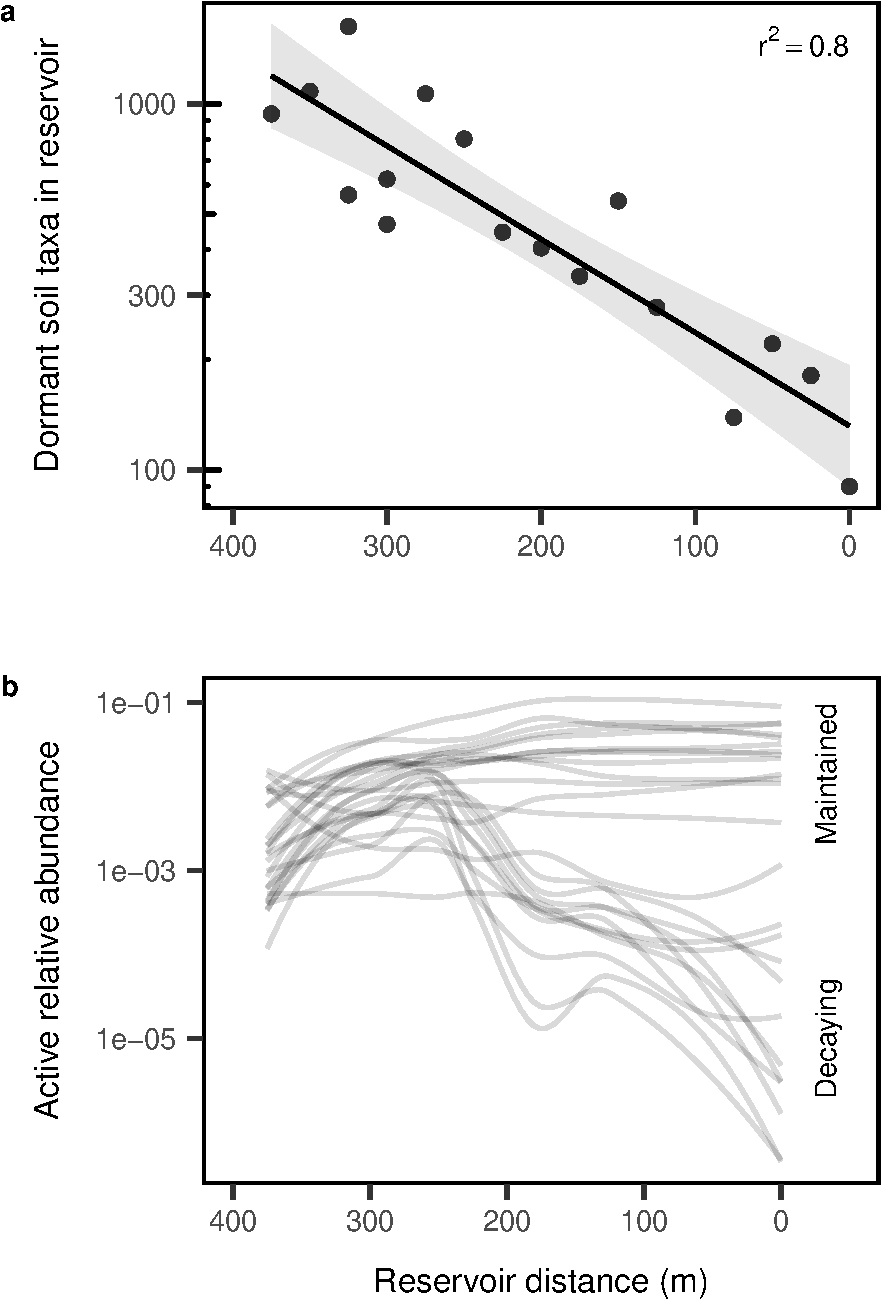
\includegraphics{ReservoirGradient_files/figure-latex/fate_panel-1} \end{center}

\hypertarget{figure-s4-see-which-taxa-are-shared-between-habitats}{%
\section{Figure S4: See which taxa are shared between
habitats}\label{figure-s4-see-which-taxa-are-shared-between-habitats}}

\begin{Shaded}
\begin{Highlighting}[]
\NormalTok{OTUs.PA <-}\StringTok{ }\KeywordTok{decostand}\NormalTok{(OTUsREL, }\DataTypeTok{method =} \StringTok{"pa"}\NormalTok{)}
\NormalTok{soil <-}\StringTok{ }\KeywordTok{names}\NormalTok{(}\KeywordTok{which}\NormalTok{(}\KeywordTok{colSums}\NormalTok{(OTUs.PA[design}\OperatorTok{$}\NormalTok{type }\OperatorTok{==}\StringTok{ "soil"}\NormalTok{,]) }\OperatorTok{>}\StringTok{ }\DecValTok{0}\NormalTok{))}
\NormalTok{water.dna <-}\StringTok{ }\KeywordTok{names}\NormalTok{(}\KeywordTok{which}\NormalTok{(}\KeywordTok{colSums}\NormalTok{(OTUs.PA[design}\OperatorTok{$}\NormalTok{type }\OperatorTok{==}\StringTok{ "water"} \OperatorTok{&}\StringTok{ }\NormalTok{design}\OperatorTok{$}\NormalTok{molecule }\OperatorTok{==}\StringTok{ "DNA"}\NormalTok{,]) }\OperatorTok{>}\StringTok{ }\DecValTok{0}\NormalTok{))}
\NormalTok{water.rna <-}\StringTok{ }\KeywordTok{names}\NormalTok{(}\KeywordTok{which}\NormalTok{(}\KeywordTok{colSums}\NormalTok{(OTUs.PA[design}\OperatorTok{$}\NormalTok{type }\OperatorTok{==}\StringTok{ "water"} \OperatorTok{&}\StringTok{ }\NormalTok{design}\OperatorTok{$}\NormalTok{molecule }\OperatorTok{==}\StringTok{ "RNA"}\NormalTok{,]) }\OperatorTok{>}\StringTok{ }\DecValTok{0}\NormalTok{))}

\KeywordTok{sum}\NormalTok{(water.rna }\OperatorTok\StringTok{ }\NormalTok{water.dna)}
\end{Highlighting}
\end{Shaded}

\begin{verbatim}
## [1] 2085
\end{verbatim}

\begin{Shaded}
\begin{Highlighting}[]
\NormalTok{nsoil <-}\StringTok{ }\KeywordTok{length}\NormalTok{(soil)}
\NormalTok{nwdna <-}\StringTok{ }\KeywordTok{length}\NormalTok{(water.dna)}
\NormalTok{nwrna <-}\StringTok{ }\KeywordTok{length}\NormalTok{(water.rna)}
\NormalTok{otus.by.habitat <-}\StringTok{ }\KeywordTok{list}\NormalTok{(}\StringTok{"Soil"}\NormalTok{ =}\StringTok{ }\NormalTok{soil, }\StringTok{"Total Aquatic"}\NormalTok{ =}\StringTok{ }\NormalTok{water.dna, }\StringTok{"Active Aquatic"}\NormalTok{ =}\StringTok{ }\NormalTok{water.rna)}

\KeywordTok{venn.diagram}\NormalTok{(otus.by.habitat, }\StringTok{"figures/FigureS4.png"}\NormalTok{, }
             \DataTypeTok{imagetype =} \StringTok{"png"}\NormalTok{, }
             \DataTypeTok{fontfamily =} \StringTok{"sans"}\NormalTok{, }
             \DataTypeTok{cat.fontfamily =} \StringTok{"sans"}\NormalTok{,}
             \DataTypeTok{alpha =} \FloatTok{.25}\NormalTok{)}
\end{Highlighting}
\end{Shaded}

\begin{verbatim}
## [1] 1
\end{verbatim}

\hypertarget{figure-s2-threshold-for-cutoffs-in-occupancy-fraction}{%
\section{Figure S2: Threshold for cutoffs in occupancy
fraction}\label{figure-s2-threshold-for-cutoffs-in-occupancy-fraction}}

\begin{Shaded}
\begin{Highlighting}[]
\CommentTok{# identify otus in soil samples and lake samples}
\NormalTok{in.soil <-}\StringTok{ }\NormalTok{OTUs[, }\KeywordTok{which}\NormalTok{(}\KeywordTok{colSums}\NormalTok{(OTUs[}\KeywordTok{c}\NormalTok{(}\DecValTok{1}\OperatorTok{:}\DecValTok{3}\NormalTok{),]) }\OperatorTok{>}\StringTok{ }\DecValTok{0}\NormalTok{ )]}

\CommentTok{# isolate just the rna water samples and convert to presence-absence}
\NormalTok{in.lake.rna <-}\StringTok{ }\NormalTok{OTUs[}\KeywordTok{which}\NormalTok{(design}\OperatorTok{$}\NormalTok{molecule }\OperatorTok{==}\StringTok{ "RNA"} \OperatorTok{&}\StringTok{ }\NormalTok{design}\OperatorTok{$}\NormalTok{type }\OperatorTok{==}\StringTok{ "water"}\NormalTok{), ]}
\NormalTok{in.lake.rna.pa <-}\StringTok{ }\NormalTok{(in.lake.rna }\OperatorTok{>}\StringTok{ }\DecValTok{0}\NormalTok{) }\OperatorTok{*}\StringTok{ }\DecValTok{1}

\NormalTok{threshlist <-}\StringTok{ }\KeywordTok{c}\NormalTok{(.}\DecValTok{3}\NormalTok{, }\FloatTok{.4}\NormalTok{, }\FloatTok{.5}\NormalTok{, }\FloatTok{.6}\NormalTok{, }\FloatTok{.7}\NormalTok{, }\FloatTok{.8}\NormalTok{, }\FloatTok{.9}\NormalTok{)}
\NormalTok{df.plot <-}\StringTok{ }\KeywordTok{data.frame}\NormalTok{()}
\ControlFlowTok{for}\NormalTok{(thresh }\ControlFlowTok{in}\NormalTok{ threshlist)\{}
  \CommentTok{# define the 'core' taxa as otus present in 50% of samples}
\NormalTok{in.lake.core <-}\StringTok{ }\NormalTok{w.dna[, }\KeywordTok{which}\NormalTok{((}\KeywordTok{colSums}\NormalTok{(in.lake.rna.pa) }\OperatorTok{/}\StringTok{ }\KeywordTok{nrow}\NormalTok{(in.lake.rna.pa)) }\OperatorTok{>=}\StringTok{ }\NormalTok{thresh)]}

\CommentTok{# of the core, how many are also in the soil samples?}
\NormalTok{in.lake.core.from.soils <-}\StringTok{ }\NormalTok{in.lake.core[, }\KeywordTok{intersect}\NormalTok{(}\KeywordTok{colnames}\NormalTok{(in.lake.core), }\KeywordTok{colnames}\NormalTok{(in.soil))]}

\CommentTok{# of the core which are not in the soil samples}
\NormalTok{in.lake.core.not.soils <-}\StringTok{ }\NormalTok{in.lake.core[, }\KeywordTok{setdiff}\NormalTok{(}\KeywordTok{colnames}\NormalTok{(in.lake.core), }\KeywordTok{colnames}\NormalTok{(in.soil))]}

\CommentTok{# Find the relative abundance of the core taxa and prepare data frame to plot}
\NormalTok{in.lake.core.from.soils.REL <-}\StringTok{ }\NormalTok{in.lake.core.from.soils }\OperatorTok{/}\StringTok{ }\KeywordTok{rowSums}\NormalTok{(w.dna)}

\NormalTok{in.soil.to.plot <-}\StringTok{ }\KeywordTok{as.data.frame}\NormalTok{(in.lake.core.from.soils.REL) }\OperatorTok\StringTok{ }
\StringTok{  }\KeywordTok{rownames_to_column}\NormalTok{(}\StringTok{"sample_ID"}\NormalTok{) }\OperatorTok\StringTok{ }
\StringTok{  }\KeywordTok{gather}\NormalTok{(otu_id, rel_abundance, }\OperatorTok{-}\NormalTok{sample_ID) }\OperatorTok\StringTok{ }
\StringTok{  }\KeywordTok{left_join}\NormalTok{(}\KeywordTok{rownames_to_column}\NormalTok{(design.dna, }\StringTok{"sample_ID"}\NormalTok{)) }\OperatorTok\StringTok{ }
\StringTok{  }\KeywordTok{add_column}\NormalTok{(}\DataTypeTok{found =} \StringTok{"soils"}\NormalTok{)}

\NormalTok{in.lake.core.not.soils.REL <-}\StringTok{ }\NormalTok{in.lake.core.not.soils }\OperatorTok{/}\StringTok{ }\KeywordTok{rowSums}\NormalTok{(w.dna)}

\NormalTok{in.lake.to.plot <-}\StringTok{ }\KeywordTok{as.data.frame}\NormalTok{(in.lake.core.not.soils.REL) }\OperatorTok\StringTok{ }
\StringTok{  }\KeywordTok{rownames_to_column}\NormalTok{(}\StringTok{"sample_ID"}\NormalTok{) }\OperatorTok\StringTok{ }
\StringTok{  }\KeywordTok{gather}\NormalTok{(otu_id, rel_abundance, }\OperatorTok{-}\NormalTok{sample_ID) }\OperatorTok\StringTok{ }
\StringTok{  }\KeywordTok{left_join}\NormalTok{(}\KeywordTok{rownames_to_column}\NormalTok{(design.dna, }\StringTok{"sample_ID"}\NormalTok{)) }\OperatorTok\StringTok{ }
\StringTok{  }\KeywordTok{add_column}\NormalTok{(}\DataTypeTok{found =} \StringTok{"lake"}\NormalTok{)}

\CommentTok{# model distance effect on rel abundance to get slope and pval}
\NormalTok{soil.core.mods <-}\StringTok{ }\KeywordTok{apply}\NormalTok{(in.lake.core.from.soils.REL, }\DataTypeTok{MARGIN =} \DecValTok{2}\NormalTok{, }
    \DataTypeTok{FUN =} \ControlFlowTok{function}\NormalTok{(x) }\KeywordTok{summary}\NormalTok{(}\KeywordTok{lm}\NormalTok{(x }\OperatorTok{~}\StringTok{ }\NormalTok{design.dna}\OperatorTok{$}\NormalTok{distance))}\OperatorTok{$}\NormalTok{coefficients[}\DecValTok{2}\NormalTok{,}\KeywordTok{c}\NormalTok{(}\DecValTok{1}\NormalTok{,}\DecValTok{4}\NormalTok{)])}
\KeywordTok{rownames}\NormalTok{(soil.core.mods) <-}\StringTok{ }\KeywordTok{c}\NormalTok{(}\StringTok{"slope"}\NormalTok{, }\StringTok{"pval"}\NormalTok{)}

\CommentTok{# classify otus as significantly increasing or decreasing along reservoir}
\NormalTok{soil.core.decreasing <-}\StringTok{ }\KeywordTok{as.data.frame}\NormalTok{(}\KeywordTok{t}\NormalTok{(soil.core.mods)) }\OperatorTok\StringTok{ }
\StringTok{  }\KeywordTok{rownames_to_column}\NormalTok{(}\StringTok{"OTU"}\NormalTok{) }\OperatorTok\StringTok{ }
\StringTok{  }\KeywordTok{filter}\NormalTok{(slope }\OperatorTok{<}\StringTok{ }\DecValTok{0}\NormalTok{) }\OperatorTok\StringTok{   }\CommentTok{# rel abund decreases toward dam}
\StringTok{  }\KeywordTok{left_join}\NormalTok{(OTU.tax)}
\NormalTok{soil.core.increasing <-}\StringTok{ }\KeywordTok{as.data.frame}\NormalTok{(}\KeywordTok{t}\NormalTok{(soil.core.mods)) }\OperatorTok\StringTok{ }
\StringTok{  }\KeywordTok{rownames_to_column}\NormalTok{(}\StringTok{"OTU"}\NormalTok{) }\OperatorTok\StringTok{ }
\StringTok{  }\KeywordTok{filter}\NormalTok{(slope }\OperatorTok{>}\StringTok{ }\DecValTok{0}\NormalTok{) }\OperatorTok\StringTok{   }\CommentTok{# rel abund increases toward dam}
\StringTok{  }\KeywordTok{left_join}\NormalTok{(OTU.tax)}

\NormalTok{nonsoil.core.mods <-}\StringTok{ }\KeywordTok{apply}\NormalTok{(in.lake.core.not.soils.REL, }\DataTypeTok{MARGIN =} \DecValTok{2}\NormalTok{, }
    \DataTypeTok{FUN =} \ControlFlowTok{function}\NormalTok{(x) }\KeywordTok{summary}\NormalTok{(}\KeywordTok{lm}\NormalTok{(x }\OperatorTok{~}\StringTok{ }\NormalTok{design.dna}\OperatorTok{$}\NormalTok{distance))}\OperatorTok{$}\NormalTok{coefficients[}\DecValTok{2}\NormalTok{,}\KeywordTok{c}\NormalTok{(}\DecValTok{1}\NormalTok{,}\DecValTok{4}\NormalTok{)])}
\KeywordTok{rownames}\NormalTok{(nonsoil.core.mods) <-}\StringTok{ }\KeywordTok{c}\NormalTok{(}\StringTok{"slope"}\NormalTok{, }\StringTok{"pval"}\NormalTok{)}
\NormalTok{nonsoil.core.decreasing <-}\StringTok{ }\KeywordTok{as.data.frame}\NormalTok{(}\KeywordTok{t}\NormalTok{(nonsoil.core.mods)) }\OperatorTok\StringTok{ }
\StringTok{  }\KeywordTok{rownames_to_column}\NormalTok{(}\StringTok{"OTU"}\NormalTok{) }\OperatorTok\StringTok{ }
\StringTok{  }\KeywordTok{filter}\NormalTok{(slope }\OperatorTok{<}\StringTok{ }\DecValTok{0}\NormalTok{) }\OperatorTok\StringTok{   }\CommentTok{# rel abund decreases toward dam}
\StringTok{  }\KeywordTok{left_join}\NormalTok{(OTU.tax)}
\NormalTok{nonsoil.core.increasing <-}\StringTok{ }\KeywordTok{as.data.frame}\NormalTok{(}\KeywordTok{t}\NormalTok{(nonsoil.core.mods)) }\OperatorTok\StringTok{ }
\StringTok{  }\KeywordTok{rownames_to_column}\NormalTok{(}\StringTok{"OTU"}\NormalTok{) }\OperatorTok\StringTok{ }
\StringTok{  }\KeywordTok{filter}\NormalTok{(slope }\OperatorTok{>}\StringTok{ }\DecValTok{0}\NormalTok{) }\OperatorTok\StringTok{   }\CommentTok{# rel abund increases toward dam}
\StringTok{  }\KeywordTok{left_join}\NormalTok{(OTU.tax)}

\NormalTok{df1 <-}\StringTok{ }\KeywordTok{as.data.frame}\NormalTok{(OTUsREL[,nonsoil.core.increasing}\OperatorTok{$}\NormalTok{OTU]) }\OperatorTok\StringTok{ }
\StringTok{  }\KeywordTok{rownames_to_column}\NormalTok{(}\StringTok{"sampleID"}\NormalTok{) }\OperatorTok\StringTok{ }
\StringTok{  }\KeywordTok{left_join}\NormalTok{(}\KeywordTok{rownames_to_column}\NormalTok{(design, }\StringTok{"sampleID"}\NormalTok{)) }\OperatorTok\StringTok{ }
\StringTok{  }\KeywordTok{gather}\NormalTok{(OTU, rel_abund, }\OperatorTok{-}\NormalTok{station, }\OperatorTok{-}\NormalTok{molecule, }\OperatorTok{-}\NormalTok{type, }\OperatorTok{-}\NormalTok{distance, }\OperatorTok{-}\NormalTok{sampleID) }\OperatorTok\StringTok{ }
\StringTok{  }\KeywordTok{filter}\NormalTok{(molecule }\OperatorTok{==}\StringTok{ "DNA"}\NormalTok{) }\OperatorTok\StringTok{ }\KeywordTok{left_join}\NormalTok{(OTU.tax) }\OperatorTok\StringTok{ }
\StringTok{  }\KeywordTok{mutate}\NormalTok{(}\DataTypeTok{soils =} \StringTok{"Absent from soils"}\NormalTok{, }\DataTypeTok{change =} \StringTok{"Increasing"}\NormalTok{)}
\NormalTok{n1 <-}\StringTok{ }\KeywordTok{length}\NormalTok{(}\KeywordTok{unique}\NormalTok{(df1}\OperatorTok{$}\NormalTok{OTU))}

\NormalTok{df2 <-}\StringTok{ }\KeywordTok{as.data.frame}\NormalTok{(OTUsREL[,soil.core.increasing}\OperatorTok{$}\NormalTok{OTU]) }\OperatorTok\StringTok{ }
\StringTok{  }\KeywordTok{rownames_to_column}\NormalTok{(}\StringTok{"sampleID"}\NormalTok{) }\OperatorTok\StringTok{ }
\StringTok{  }\KeywordTok{left_join}\NormalTok{(}\KeywordTok{rownames_to_column}\NormalTok{(design, }\StringTok{"sampleID"}\NormalTok{)) }\OperatorTok\StringTok{ }
\StringTok{  }\KeywordTok{gather}\NormalTok{(OTU, rel_abund, }\OperatorTok{-}\NormalTok{station, }\OperatorTok{-}\NormalTok{molecule, }\OperatorTok{-}\NormalTok{type, }\OperatorTok{-}\NormalTok{distance, }\OperatorTok{-}\NormalTok{sampleID) }\OperatorTok\StringTok{ }
\StringTok{  }\KeywordTok{filter}\NormalTok{(molecule }\OperatorTok{==}\StringTok{ "DNA"}\NormalTok{) }\OperatorTok\StringTok{ }\KeywordTok{left_join}\NormalTok{(OTU.tax) }\OperatorTok\StringTok{ }
\StringTok{  }\KeywordTok{mutate}\NormalTok{(}\DataTypeTok{soils =} \StringTok{"Present in soils"}\NormalTok{, }\DataTypeTok{change =} \StringTok{"Increasing"}\NormalTok{)}
\NormalTok{n2 <-}\StringTok{ }\KeywordTok{length}\NormalTok{(}\KeywordTok{unique}\NormalTok{(df2}\OperatorTok{$}\NormalTok{OTU))}

\NormalTok{df3 <-}\StringTok{ }\KeywordTok{as.data.frame}\NormalTok{(OTUsREL[,soil.core.decreasing}\OperatorTok{$}\NormalTok{OTU]) }\OperatorTok\StringTok{ }
\StringTok{  }\KeywordTok{rownames_to_column}\NormalTok{(}\StringTok{"sampleID"}\NormalTok{) }\OperatorTok\StringTok{ }
\StringTok{  }\KeywordTok{left_join}\NormalTok{(}\KeywordTok{rownames_to_column}\NormalTok{(design, }\StringTok{"sampleID"}\NormalTok{)) }\OperatorTok\StringTok{ }
\StringTok{  }\KeywordTok{gather}\NormalTok{(OTU, rel_abund, }\OperatorTok{-}\NormalTok{station, }\OperatorTok{-}\NormalTok{molecule, }\OperatorTok{-}\NormalTok{type, }\OperatorTok{-}\NormalTok{distance, }\OperatorTok{-}\NormalTok{sampleID) }\OperatorTok\StringTok{ }
\StringTok{  }\KeywordTok{filter}\NormalTok{(molecule }\OperatorTok{==}\StringTok{ "DNA"}\NormalTok{) }\OperatorTok\StringTok{ }\KeywordTok{left_join}\NormalTok{(OTU.tax) }\OperatorTok\StringTok{ }
\StringTok{  }\KeywordTok{mutate}\NormalTok{(}\DataTypeTok{soils =} \StringTok{"Present in soils"}\NormalTok{, }\DataTypeTok{change =} \StringTok{"Decreasing"}\NormalTok{)}
\NormalTok{n3 <-}\StringTok{ }\KeywordTok{length}\NormalTok{(}\KeywordTok{unique}\NormalTok{(df3}\OperatorTok{$}\NormalTok{OTU))}

\NormalTok{df4 <-}\StringTok{ }\KeywordTok{as.data.frame}\NormalTok{(OTUsREL[,nonsoil.core.decreasing}\OperatorTok{$}\NormalTok{OTU]) }\OperatorTok\StringTok{ }
\StringTok{  }\KeywordTok{rownames_to_column}\NormalTok{(}\StringTok{"sampleID"}\NormalTok{) }\OperatorTok\StringTok{ }
\StringTok{  }\KeywordTok{left_join}\NormalTok{(}\KeywordTok{rownames_to_column}\NormalTok{(design, }\StringTok{"sampleID"}\NormalTok{)) }\OperatorTok\StringTok{ }
\StringTok{  }\KeywordTok{gather}\NormalTok{(OTU, rel_abund, }\OperatorTok{-}\NormalTok{station, }\OperatorTok{-}\NormalTok{molecule, }\OperatorTok{-}\NormalTok{type, }\OperatorTok{-}\NormalTok{distance, }\OperatorTok{-}\NormalTok{sampleID) }\OperatorTok\StringTok{ }
\StringTok{  }\KeywordTok{filter}\NormalTok{(molecule }\OperatorTok{==}\StringTok{ "DNA"}\NormalTok{) }\OperatorTok\StringTok{ }\KeywordTok{left_join}\NormalTok{(OTU.tax) }\OperatorTok\StringTok{ }
\StringTok{  }\KeywordTok{mutate}\NormalTok{(}\DataTypeTok{soils =} \StringTok{"Absent from soils"}\NormalTok{, }\DataTypeTok{change =} \StringTok{"Decreasing"}\NormalTok{)}
\NormalTok{n4 <-}\StringTok{ }\KeywordTok{length}\NormalTok{(}\KeywordTok{unique}\NormalTok{(df4}\OperatorTok{$}\NormalTok{OTU))}


\NormalTok{df.plot <-}\StringTok{ }\KeywordTok{as_tibble}\NormalTok{(}\KeywordTok{rbind.data.frame}\NormalTok{(df1, df2, df3, df4)) }\OperatorTok\StringTok{ }
\StringTok{  }\KeywordTok{mutate}\NormalTok{(}\DataTypeTok{thresh =}\NormalTok{ thresh) }\OperatorTok\StringTok{ }\KeywordTok{filter}\NormalTok{(type }\OperatorTok{==}\StringTok{ "water"}\NormalTok{) }\OperatorTok\StringTok{ }
\StringTok{  }\KeywordTok{bind_rows}\NormalTok{(df.plot)}

\NormalTok{\}}
\end{Highlighting}
\end{Shaded}

\begin{verbatim}
## Warning: Column `OTU` joining character vector and factor, coercing into
## character vector

## Warning: Column `OTU` joining character vector and factor, coercing into
## character vector

## Warning: Column `OTU` joining character vector and factor, coercing into
## character vector

## Warning: Column `OTU` joining character vector and factor, coercing into
## character vector

## Warning: Column `OTU` joining character vector and factor, coercing into
## character vector

## Warning: Column `OTU` joining character vector and factor, coercing into
## character vector

## Warning: Column `OTU` joining character vector and factor, coercing into
## character vector

## Warning: Column `OTU` joining character vector and factor, coercing into
## character vector

## Warning: Column `OTU` joining character vector and factor, coercing into
## character vector

## Warning: Column `OTU` joining character vector and factor, coercing into
## character vector

## Warning: Column `OTU` joining character vector and factor, coercing into
## character vector

## Warning: Column `OTU` joining character vector and factor, coercing into
## character vector

## Warning: Column `OTU` joining character vector and factor, coercing into
## character vector

## Warning: Column `OTU` joining character vector and factor, coercing into
## character vector

## Warning: Column `OTU` joining character vector and factor, coercing into
## character vector

## Warning: Column `OTU` joining character vector and factor, coercing into
## character vector

## Warning: Column `OTU` joining character vector and factor, coercing into
## character vector

## Warning: Column `OTU` joining character vector and factor, coercing into
## character vector

## Warning: Column `OTU` joining character vector and factor, coercing into
## character vector

## Warning: Column `OTU` joining character vector and factor, coercing into
## character vector

## Warning: Column `OTU` joining character vector and factor, coercing into
## character vector

## Warning: Column `OTU` joining character vector and factor, coercing into
## character vector

## Warning: Column `OTU` joining character vector and factor, coercing into
## character vector

## Warning: Column `OTU` joining character vector and factor, coercing into
## character vector

## Warning: Column `OTU` joining character vector and factor, coercing into
## character vector

## Warning: Column `OTU` joining character vector and factor, coercing into
## character vector

## Warning: Column `OTU` joining character vector and factor, coercing into
## character vector

## Warning: Column `OTU` joining character vector and factor, coercing into
## character vector

## Warning: Column `OTU` joining character vector and factor, coercing into
## character vector

## Warning: Column `OTU` joining character vector and factor, coercing into
## character vector

## Warning: Column `OTU` joining character vector and factor, coercing into
## character vector

## Warning: Column `OTU` joining character vector and factor, coercing into
## character vector

## Warning: Column `OTU` joining character vector and factor, coercing into
## character vector

## Warning: Column `OTU` joining character vector and factor, coercing into
## character vector

## Warning: Column `OTU` joining character vector and factor, coercing into
## character vector

## Warning: Column `OTU` joining character vector and factor, coercing into
## character vector

## Warning: Column `OTU` joining character vector and factor, coercing into
## character vector

## Warning: Column `OTU` joining character vector and factor, coercing into
## character vector

## Warning: Column `OTU` joining character vector and factor, coercing into
## character vector

## Warning: Column `OTU` joining character vector and factor, coercing into
## character vector

## Warning: Column `OTU` joining character vector and factor, coercing into
## character vector

## Warning: Column `OTU` joining character vector and factor, coercing into
## character vector

## Warning: Column `OTU` joining character vector and factor, coercing into
## character vector

## Warning: Column `OTU` joining character vector and factor, coercing into
## character vector

## Warning: Column `OTU` joining character vector and factor, coercing into
## character vector

## Warning: Column `OTU` joining character vector and factor, coercing into
## character vector

## Warning: Column `OTU` joining character vector and factor, coercing into
## character vector

## Warning: Column `OTU` joining character vector and factor, coercing into
## character vector

## Warning: Column `OTU` joining character vector and factor, coercing into
## character vector

## Warning: Column `OTU` joining character vector and factor, coercing into
## character vector

## Warning: Column `OTU` joining character vector and factor, coercing into
## character vector

## Warning: Column `OTU` joining character vector and factor, coercing into
## character vector

## Warning: Column `OTU` joining character vector and factor, coercing into
## character vector

## Warning: Column `OTU` joining character vector and factor, coercing into
## character vector

## Warning: Column `OTU` joining character vector and factor, coercing into
## character vector

## Warning: Column `OTU` joining character vector and factor, coercing into
## character vector
\end{verbatim}

\begin{Shaded}
\begin{Highlighting}[]
\NormalTok{taxon_fate.plot <-}\StringTok{ }\NormalTok{df.plot }\OperatorTok\StringTok{ }\KeywordTok{mutate}\NormalTok{(}\DataTypeTok{rel_abund =} \KeywordTok{ifelse}\NormalTok{(rel_abund }\OperatorTok{==}\StringTok{ }\DecValTok{0}\NormalTok{, }\FloatTok{1e-6}\NormalTok{, rel_abund)) }\OperatorTok\StringTok{ }
\StringTok{  }\KeywordTok{filter}\NormalTok{(soils }\OperatorTok{==}\StringTok{ "Present in soils"}\NormalTok{) }\OperatorTok\StringTok{ }
\StringTok{  }\CommentTok{#mutate(change = ifelse(change == "Increasing", }
\StringTok{  }\CommentTok{#                       paste0("Increasing (n = ", n2,")"),}
\StringTok{  }\CommentTok{#                       paste0("Decreasing (n = ", n3,")"))) %>% }
\StringTok{  }\KeywordTok{ggplot}\NormalTok{(}\KeywordTok{aes}\NormalTok{(}\DataTypeTok{x =}\NormalTok{ distance, }\DataTypeTok{y =}\NormalTok{ rel_abund, }\DataTypeTok{group =}\NormalTok{ OTU)) }\OperatorTok{+}\StringTok{ }
\StringTok{  }\CommentTok{#geom_jitter(alpha = 0.15) + }
\StringTok{  }\KeywordTok{geom_line}\NormalTok{(}\DataTypeTok{stat =} \StringTok{"smooth"}\NormalTok{, }\DataTypeTok{alpha =} \FloatTok{0.3}\NormalTok{, }\DataTypeTok{size =} \FloatTok{.5}\NormalTok{,}
            \DataTypeTok{method =} \StringTok{"loess"}\NormalTok{, }\DataTypeTok{span =} \FloatTok{.7}\NormalTok{, }\DataTypeTok{se =} \OtherTok{FALSE}\NormalTok{) }\OperatorTok{+}
\StringTok{  }\KeywordTok{scale_y_log10}\NormalTok{(}\DataTypeTok{labels =}\NormalTok{ scales}\OperatorTok{::}\NormalTok{scientific) }\OperatorTok{+}
\StringTok{  }\KeywordTok{scale_x_continuous}\NormalTok{(}\DataTypeTok{limits =} \KeywordTok{c}\NormalTok{(}\DecValTok{0}\NormalTok{,}\DecValTok{380}\NormalTok{)) }\OperatorTok{+}
\StringTok{  }\KeywordTok{facet_wrap}\NormalTok{(}\OperatorTok{~}\NormalTok{thresh) }\OperatorTok{+}
\StringTok{  }\CommentTok{#theme(legend.position = "none") +}
\StringTok{  }\CommentTok{#guides(color = guide_legend(ncol = 1)) +}
\StringTok{  }\KeywordTok{labs}\NormalTok{(}\DataTypeTok{x =} \StringTok{"Reservoir distance (m)"}\NormalTok{,}
       \DataTypeTok{y =} \StringTok{"Active relative abundance"}\NormalTok{) }\OperatorTok{+}
\StringTok{  }\CommentTok{# annotate("text", x = 365, y = 1e-1, size = 5, hjust = 1, vjust = 1, angle = 90,}
\StringTok{  }\CommentTok{#          label = "Maintained") +}
\StringTok{  }\CommentTok{# annotate("text", x = 365, y = 1e-5, size = 5, hjust = 0.5, vjust = 1, angle = 90,}
\StringTok{  }\CommentTok{#          label = "Decaying") +}
\StringTok{  }\KeywordTok{ggsave}\NormalTok{(}\StringTok{"figures/FigureS2.pdf"}\NormalTok{, }\DataTypeTok{width =} \DecValTok{8}\NormalTok{, }\DataTypeTok{height =} \DecValTok{6}\NormalTok{, }\DataTypeTok{units =} \StringTok{"in"}\NormalTok{)}
\NormalTok{taxon_fate.plot}
\end{Highlighting}
\end{Shaded}

\begin{center}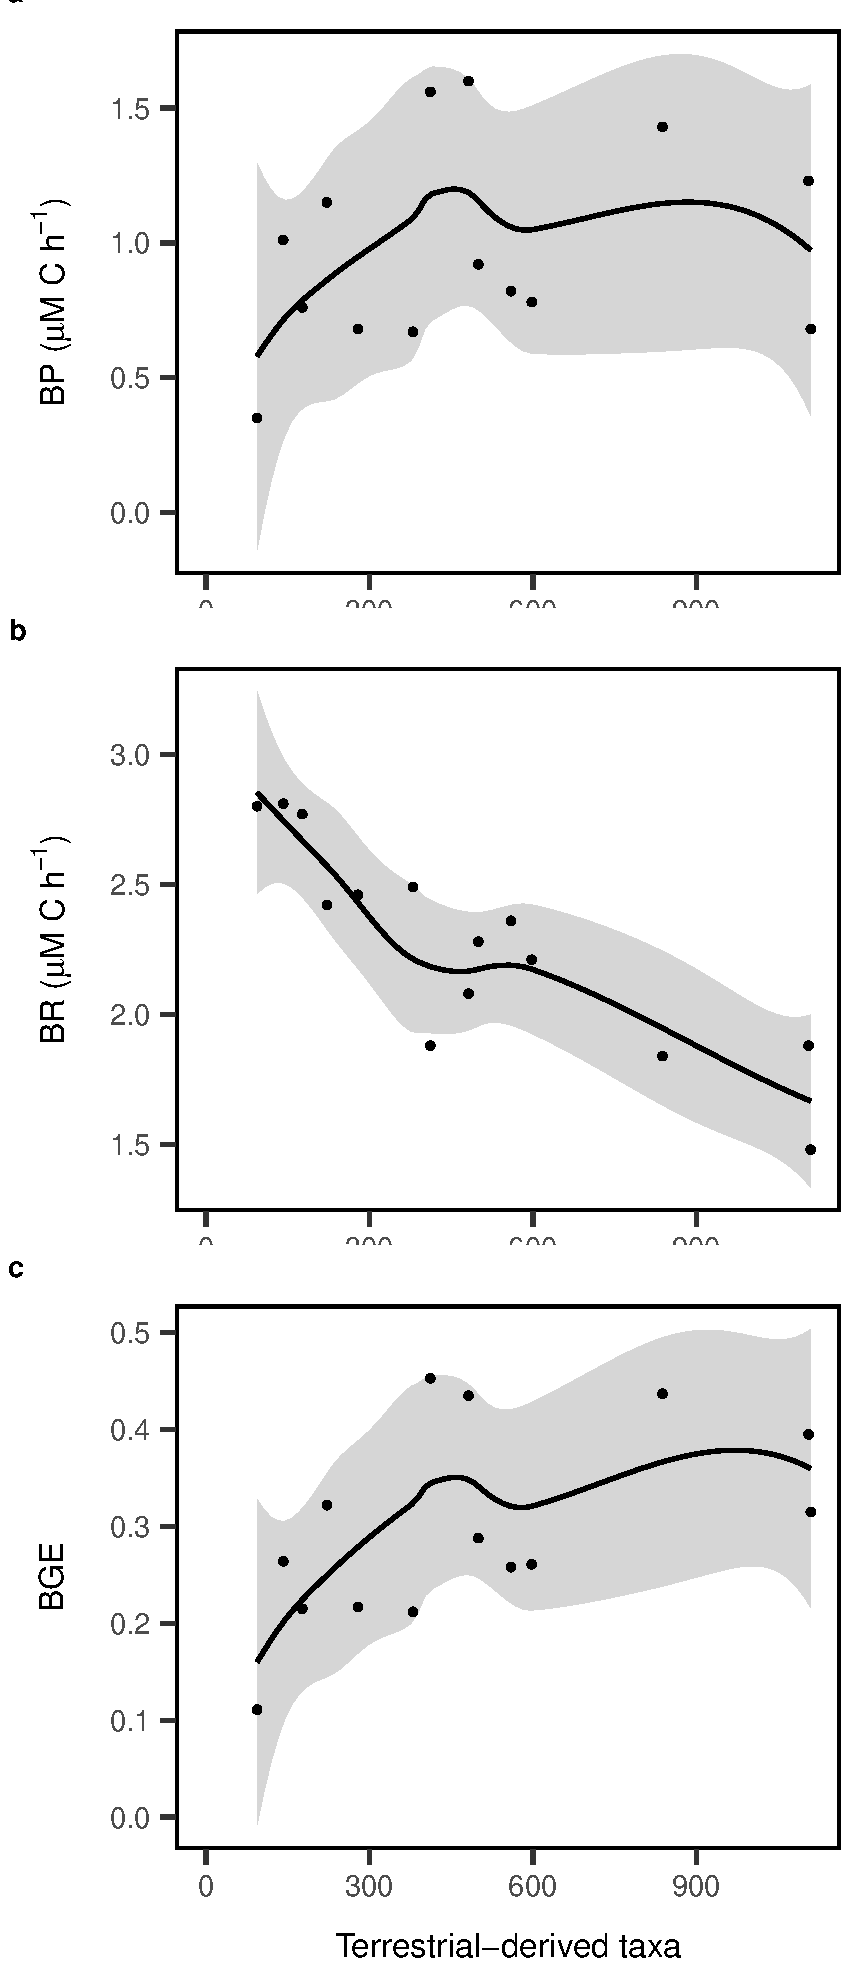
\includegraphics{ReservoirGradient_files/figure-latex/unnamed-chunk-10-1} \end{center}


\end{document}
